\clearpage
\section{Appendix A}

\subsection{Recoil}


\begin{figure}
\centering
 \subfloat{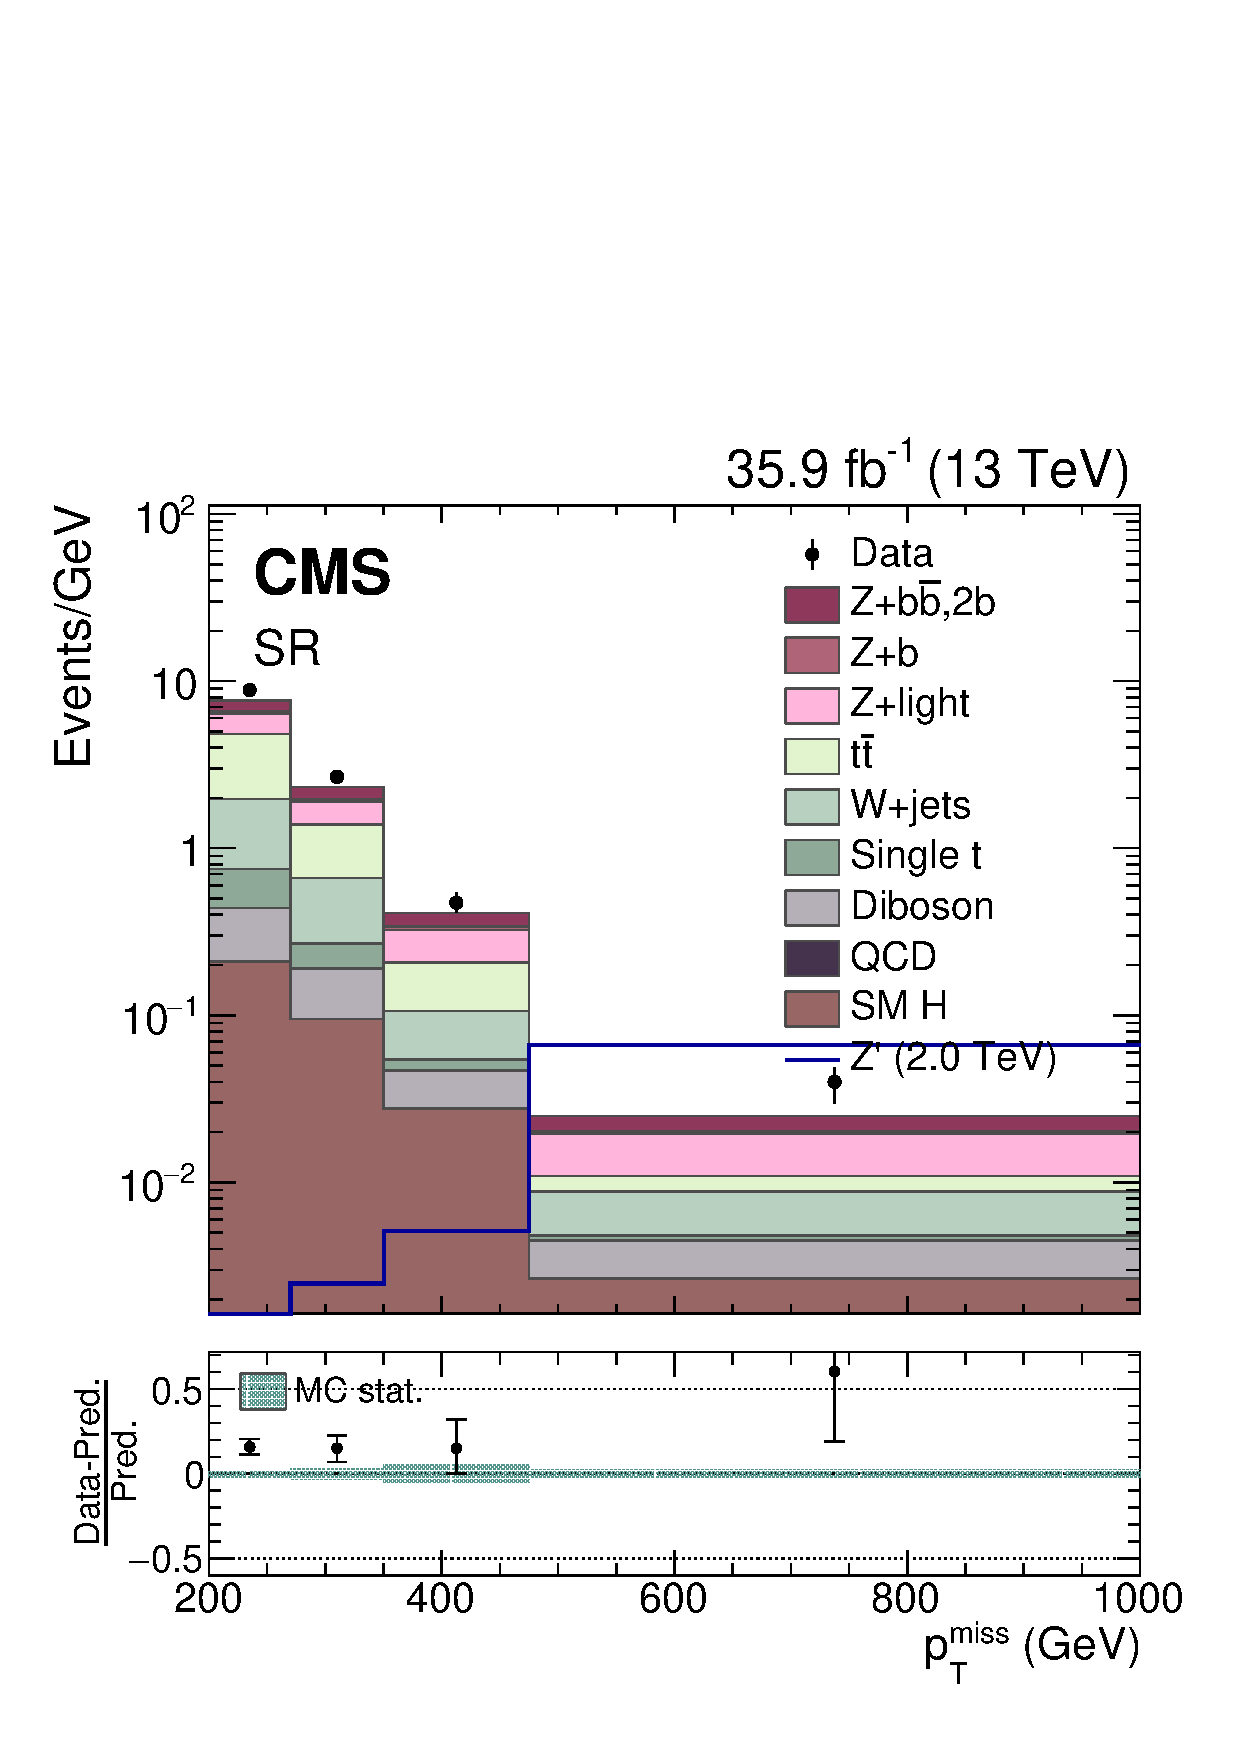
\includegraphics[width=0.45\textwidth]{figures/dataMC/sr_MET2_zcontent.pdf}}
 \subfloat{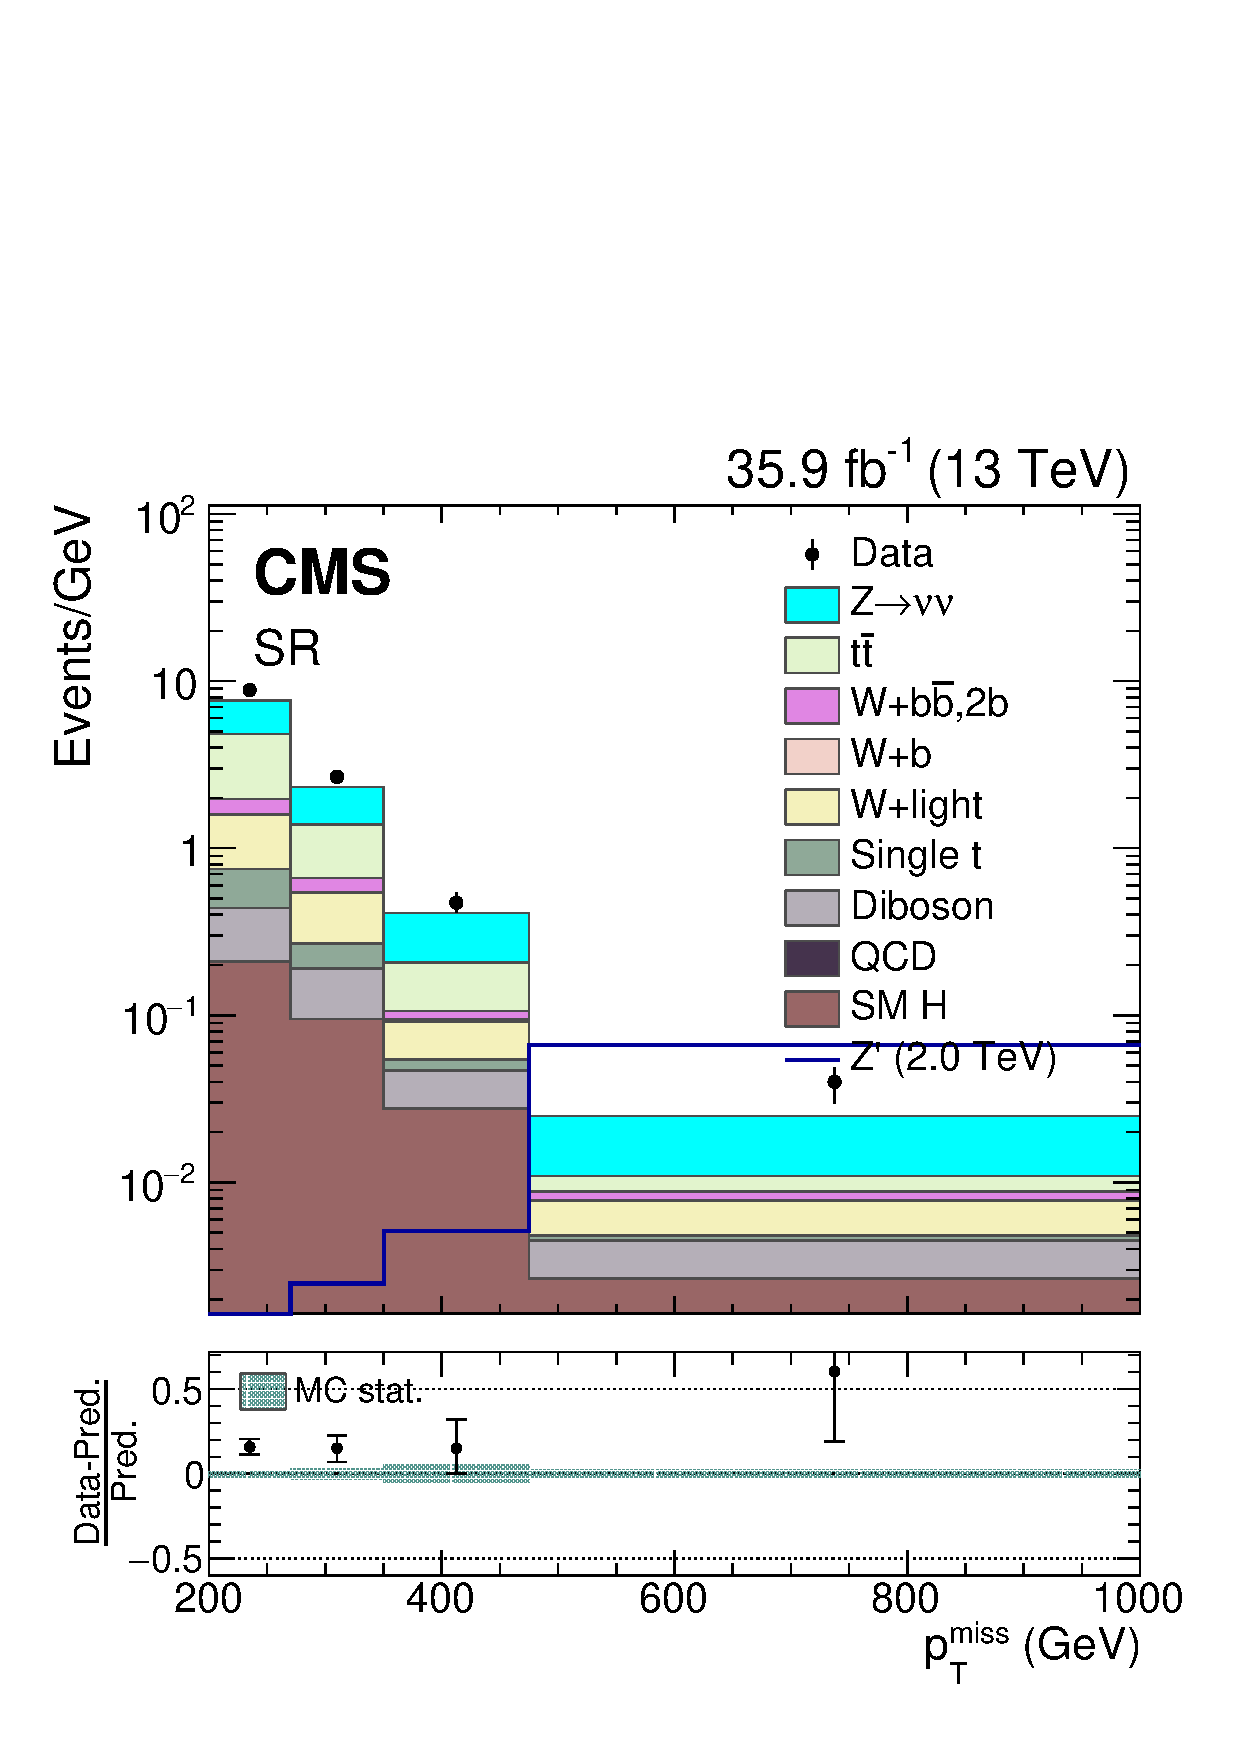
\includegraphics[width=0.45\textwidth]{figures/dataMC/sr_MET2_wcontent.pdf}}\\
 \subfloat{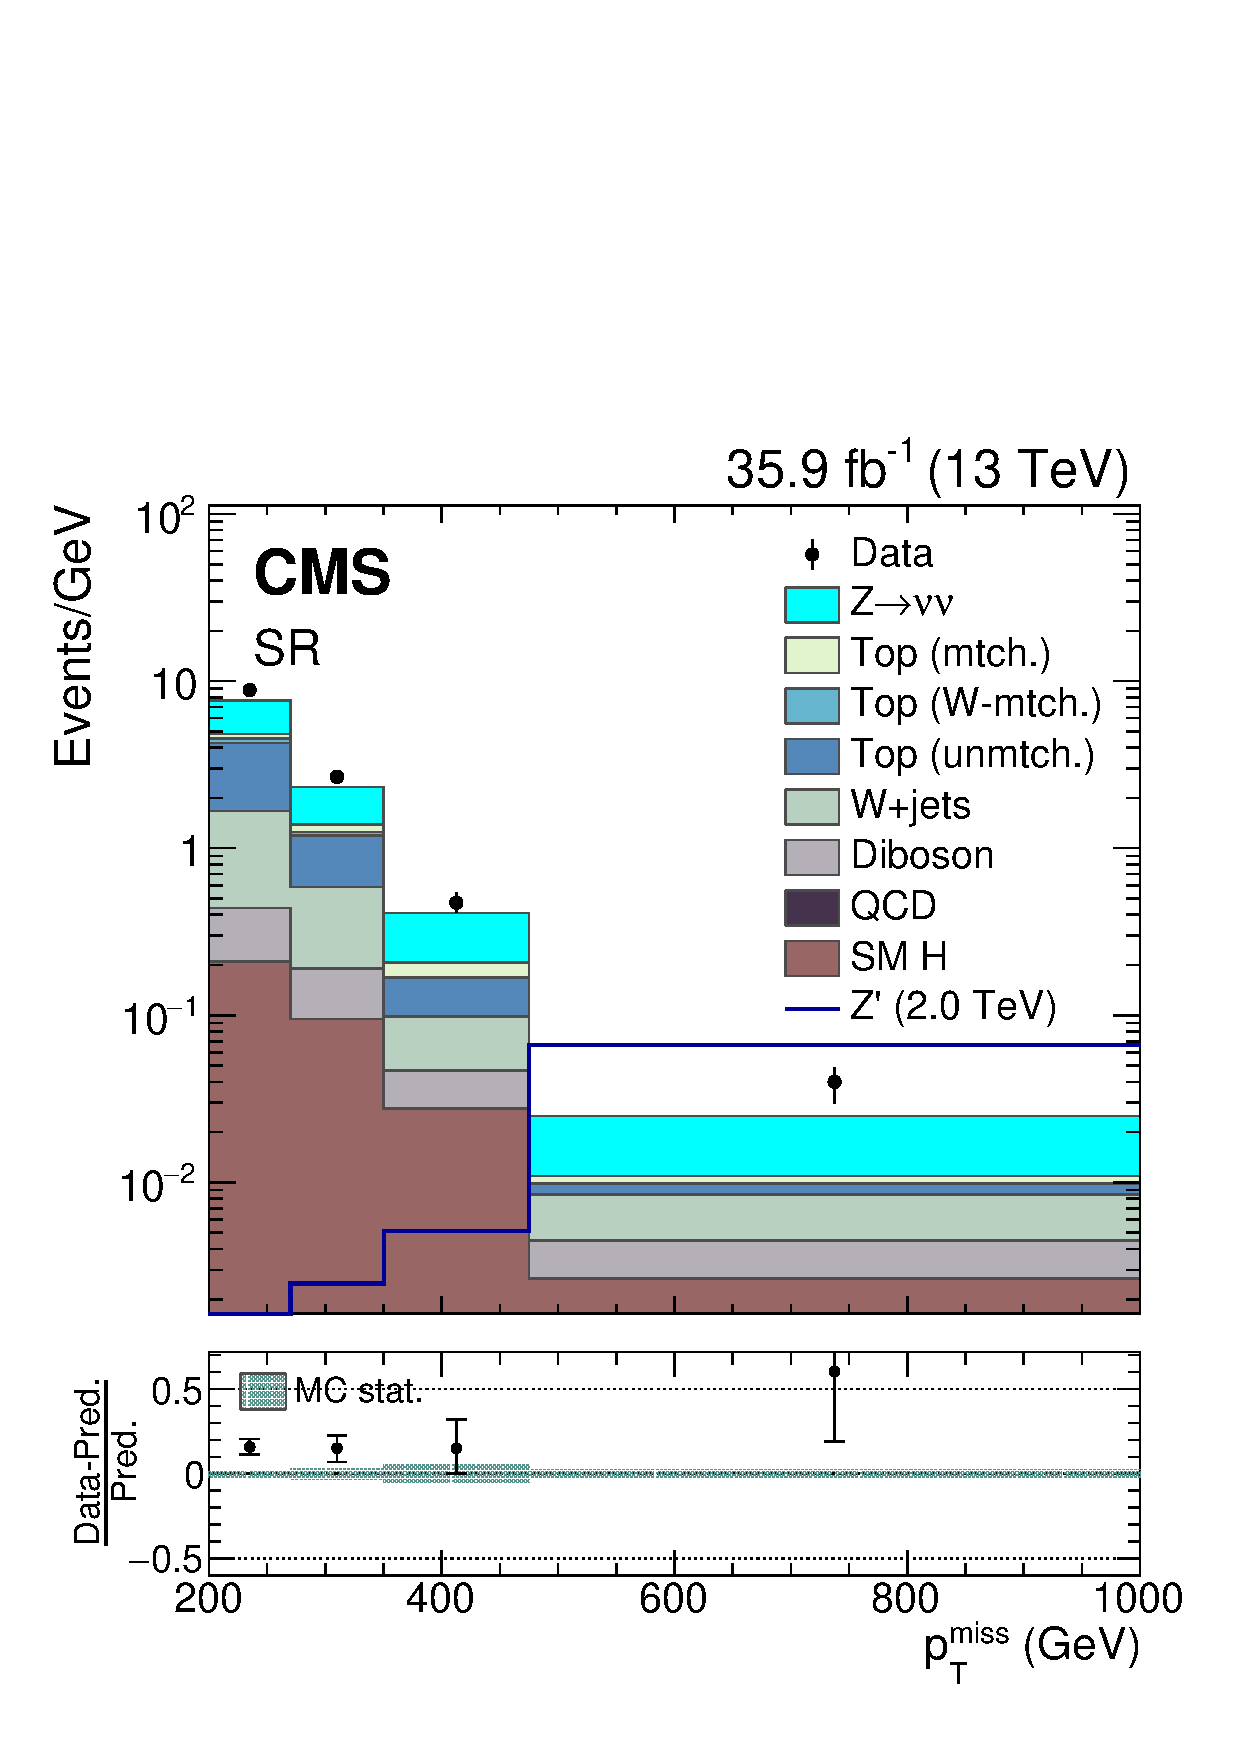
\includegraphics[width=0.45\textwidth]{figures/dataMC/sr_MET2_topcontent.pdf}}\\
\caption{The signal region distribution, with the main background split up into the fat jet quark content. For Z+jets, the $\text{b}\bar{\text{b}}$ component makes up for around 35\% of the Z+jets background (upper row, left). For W+jets, $\sim20$\% of the background comes from W+$\text{b}\bar{\text{b}}$ production (upper row, right). For \ttbar, the main contribution comes from fat jets with one b and one light quark from the W, referred to as unmatched in the legend (lower row).}
\label{Fig_sr_content}
\end{figure}

\begin{figure}
\centering
 \subfloat{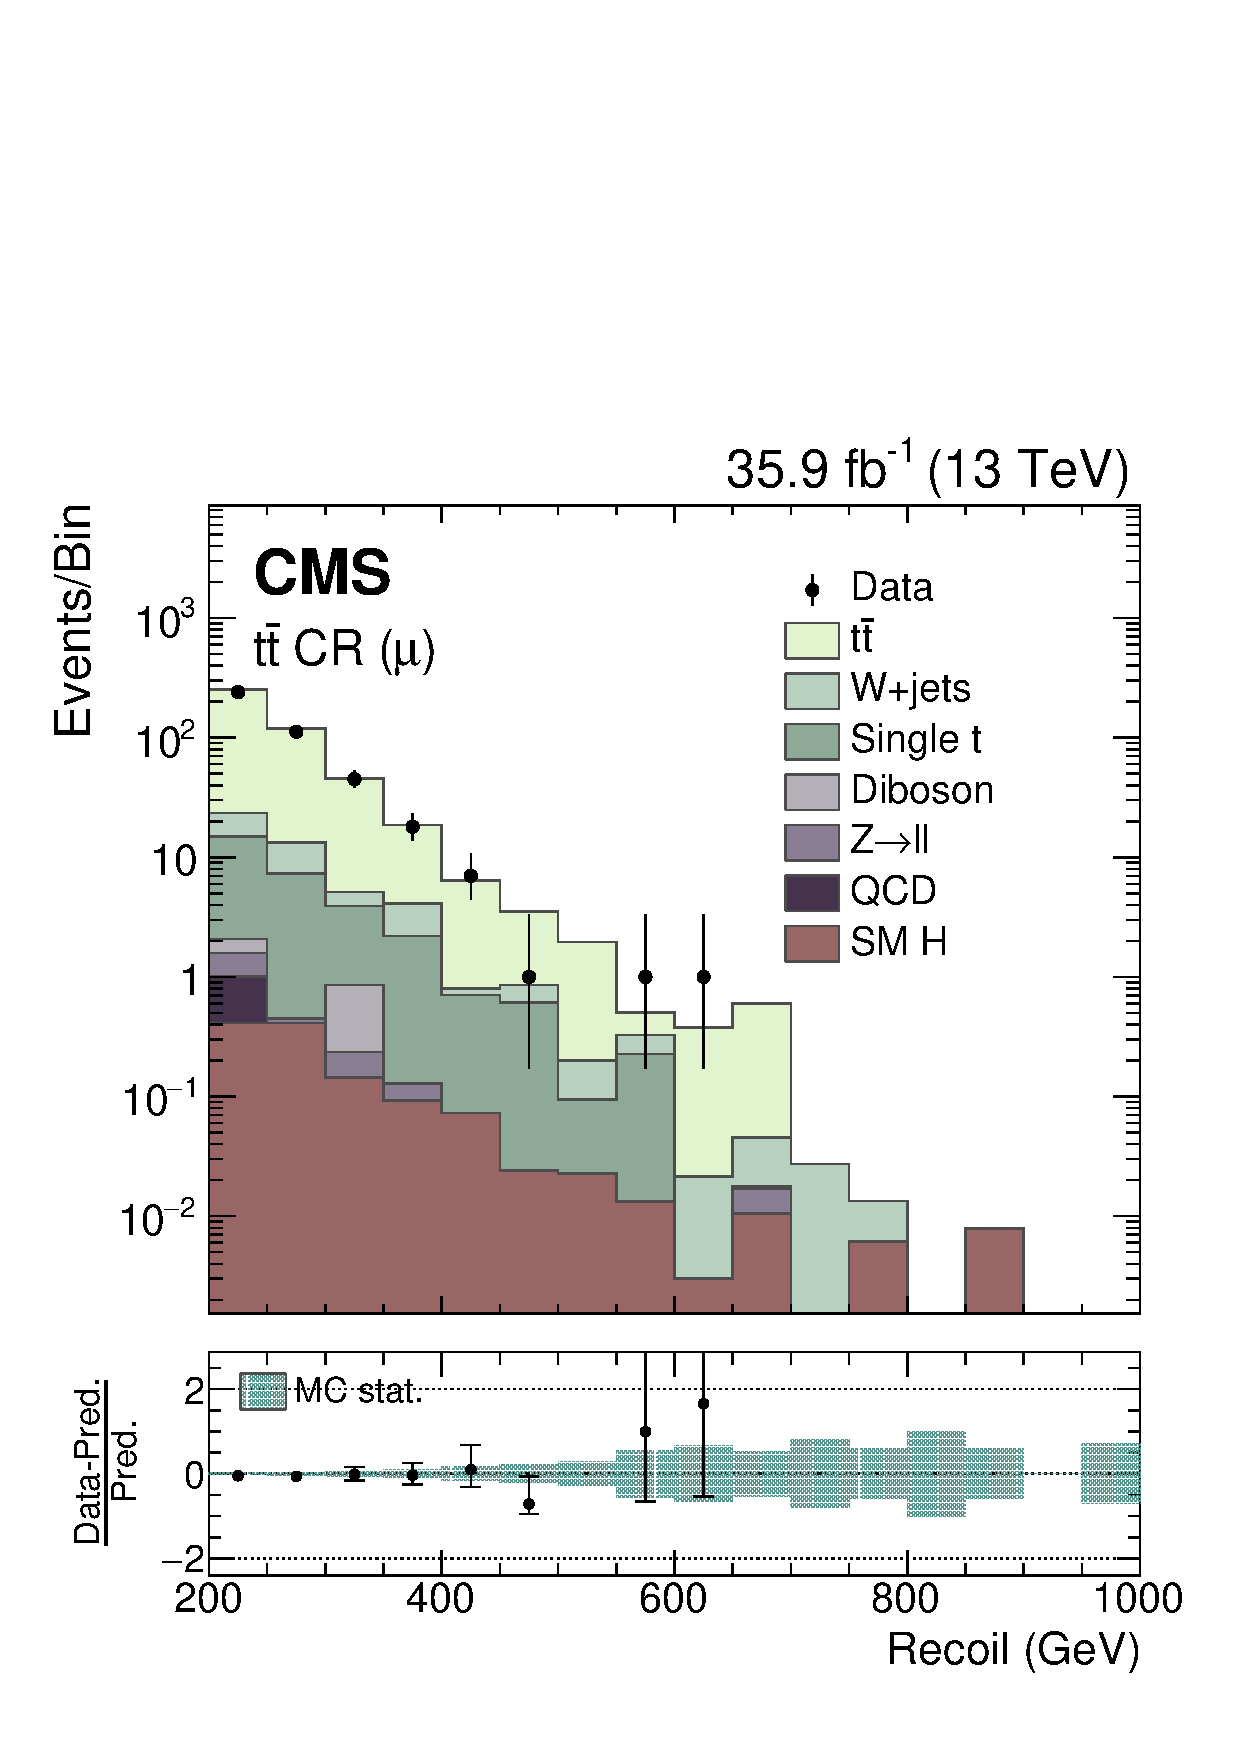
\includegraphics[width=0.4\textwidth]{figures/dataMC/cr_ttbar_mu_recoil.pdf}}
 \subfloat{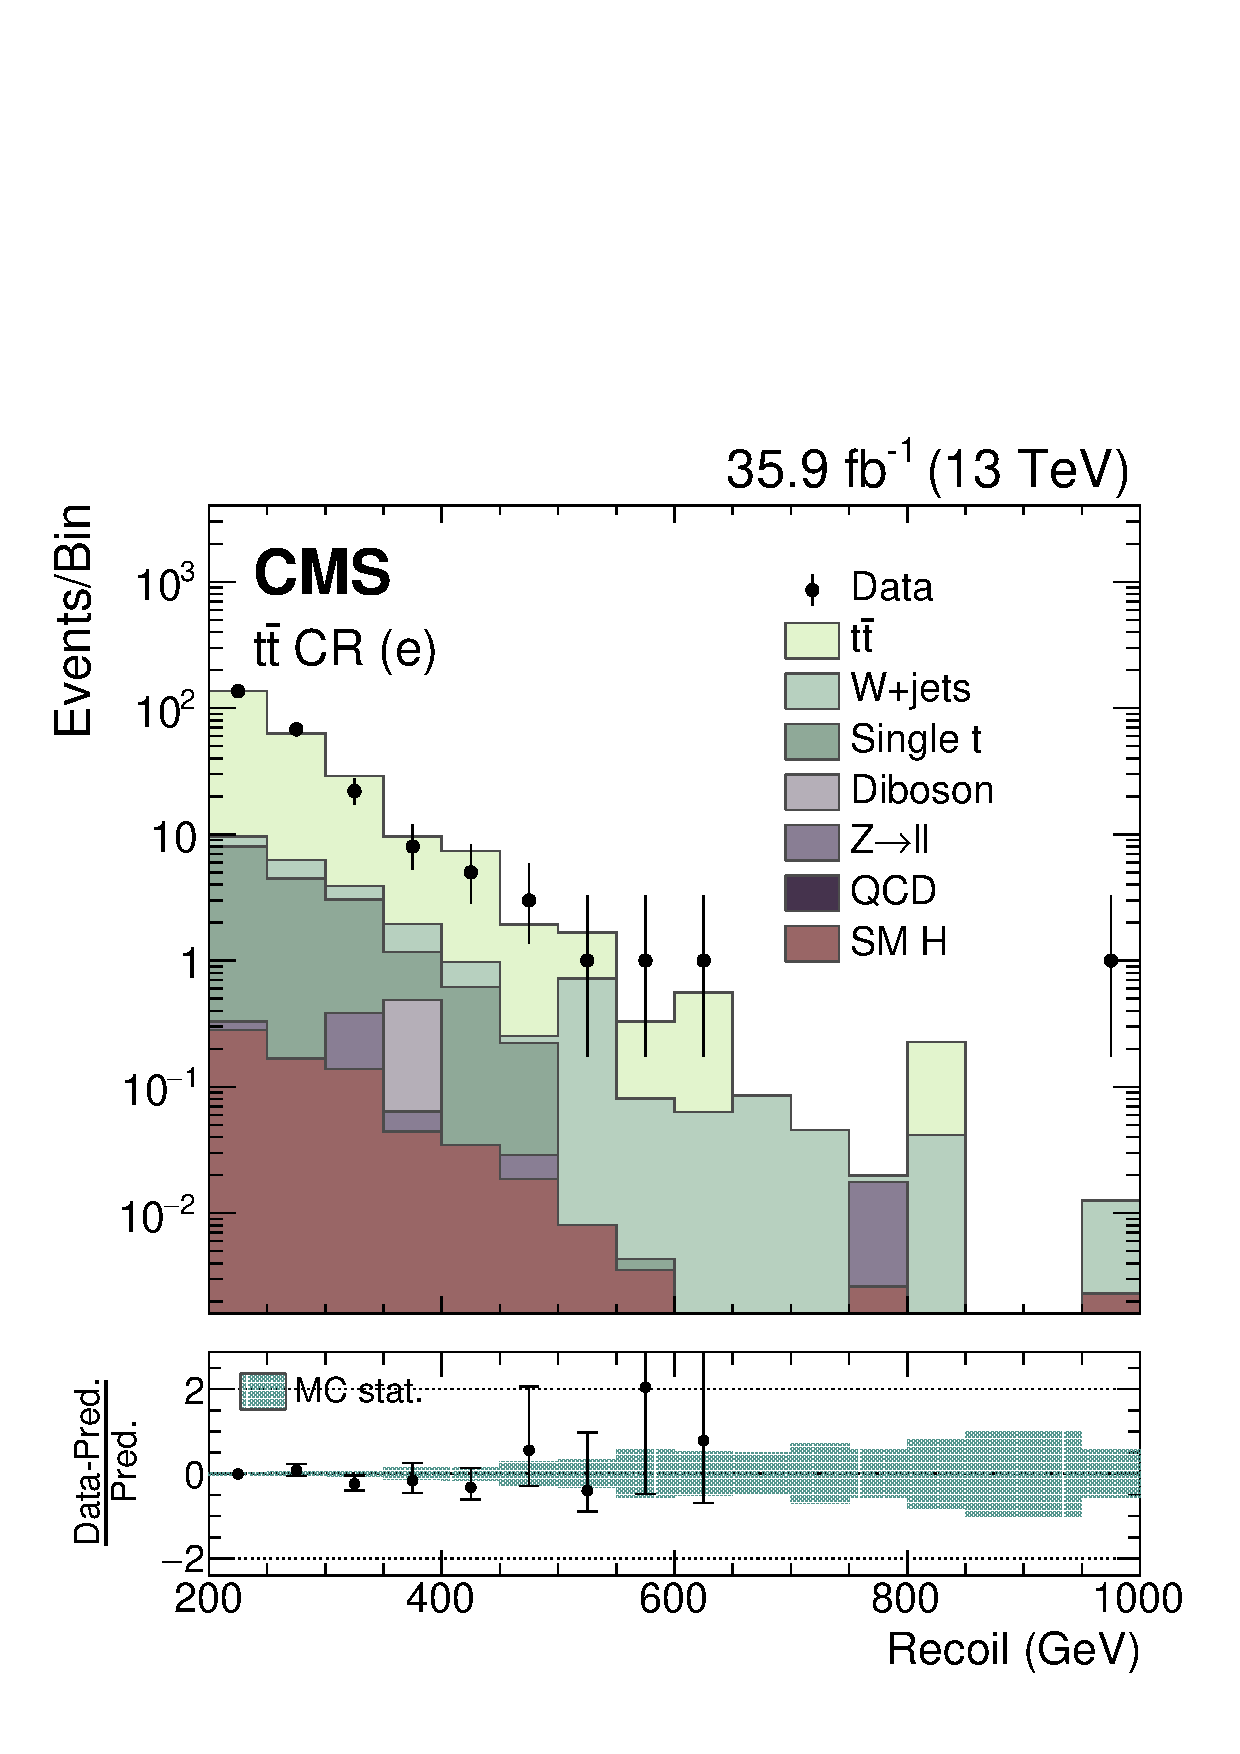
\includegraphics[width=0.4\textwidth]{figures/dataMC/cr_ttbar_el_recoil.pdf}} \\
 \subfloat{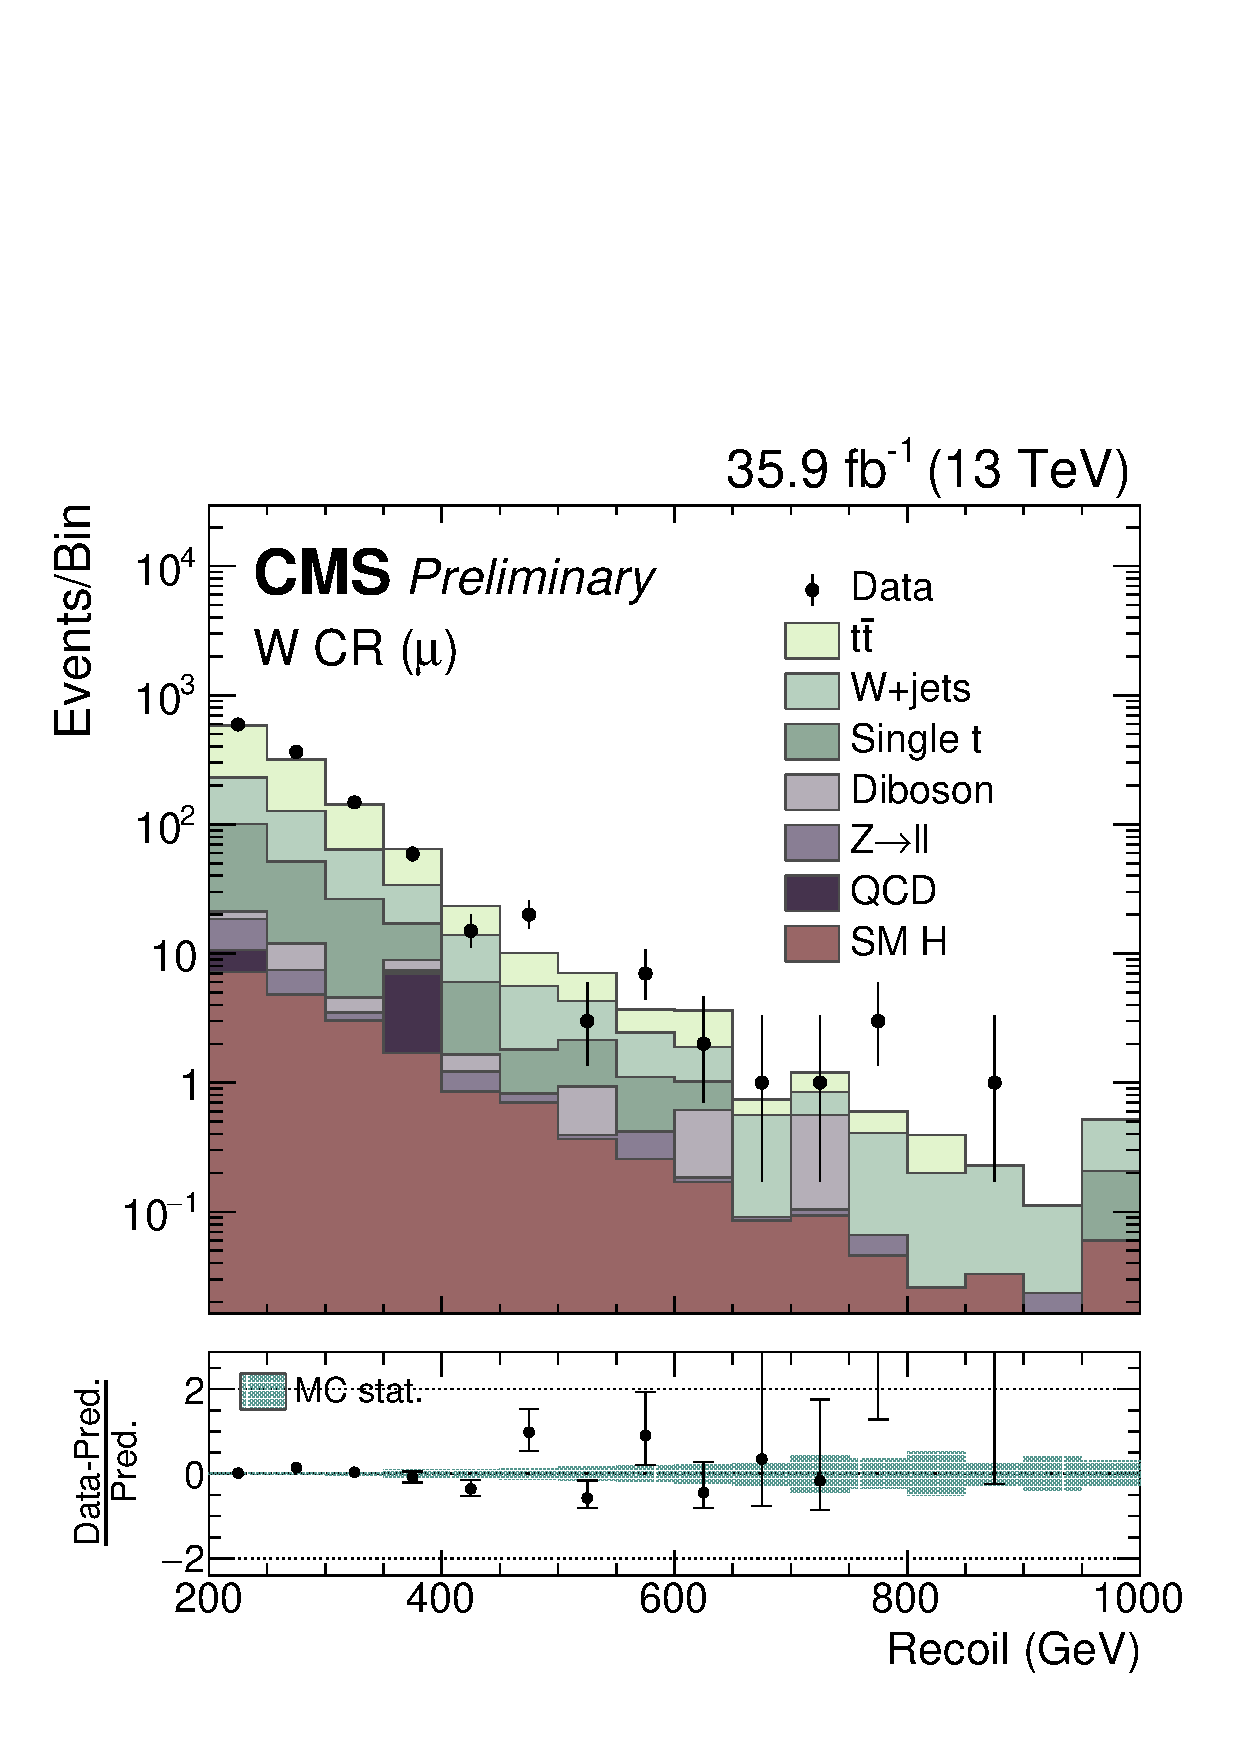
\includegraphics[width=0.4\textwidth]{figures/dataMC/cr_w_mu_recoil.pdf}}
 \subfloat{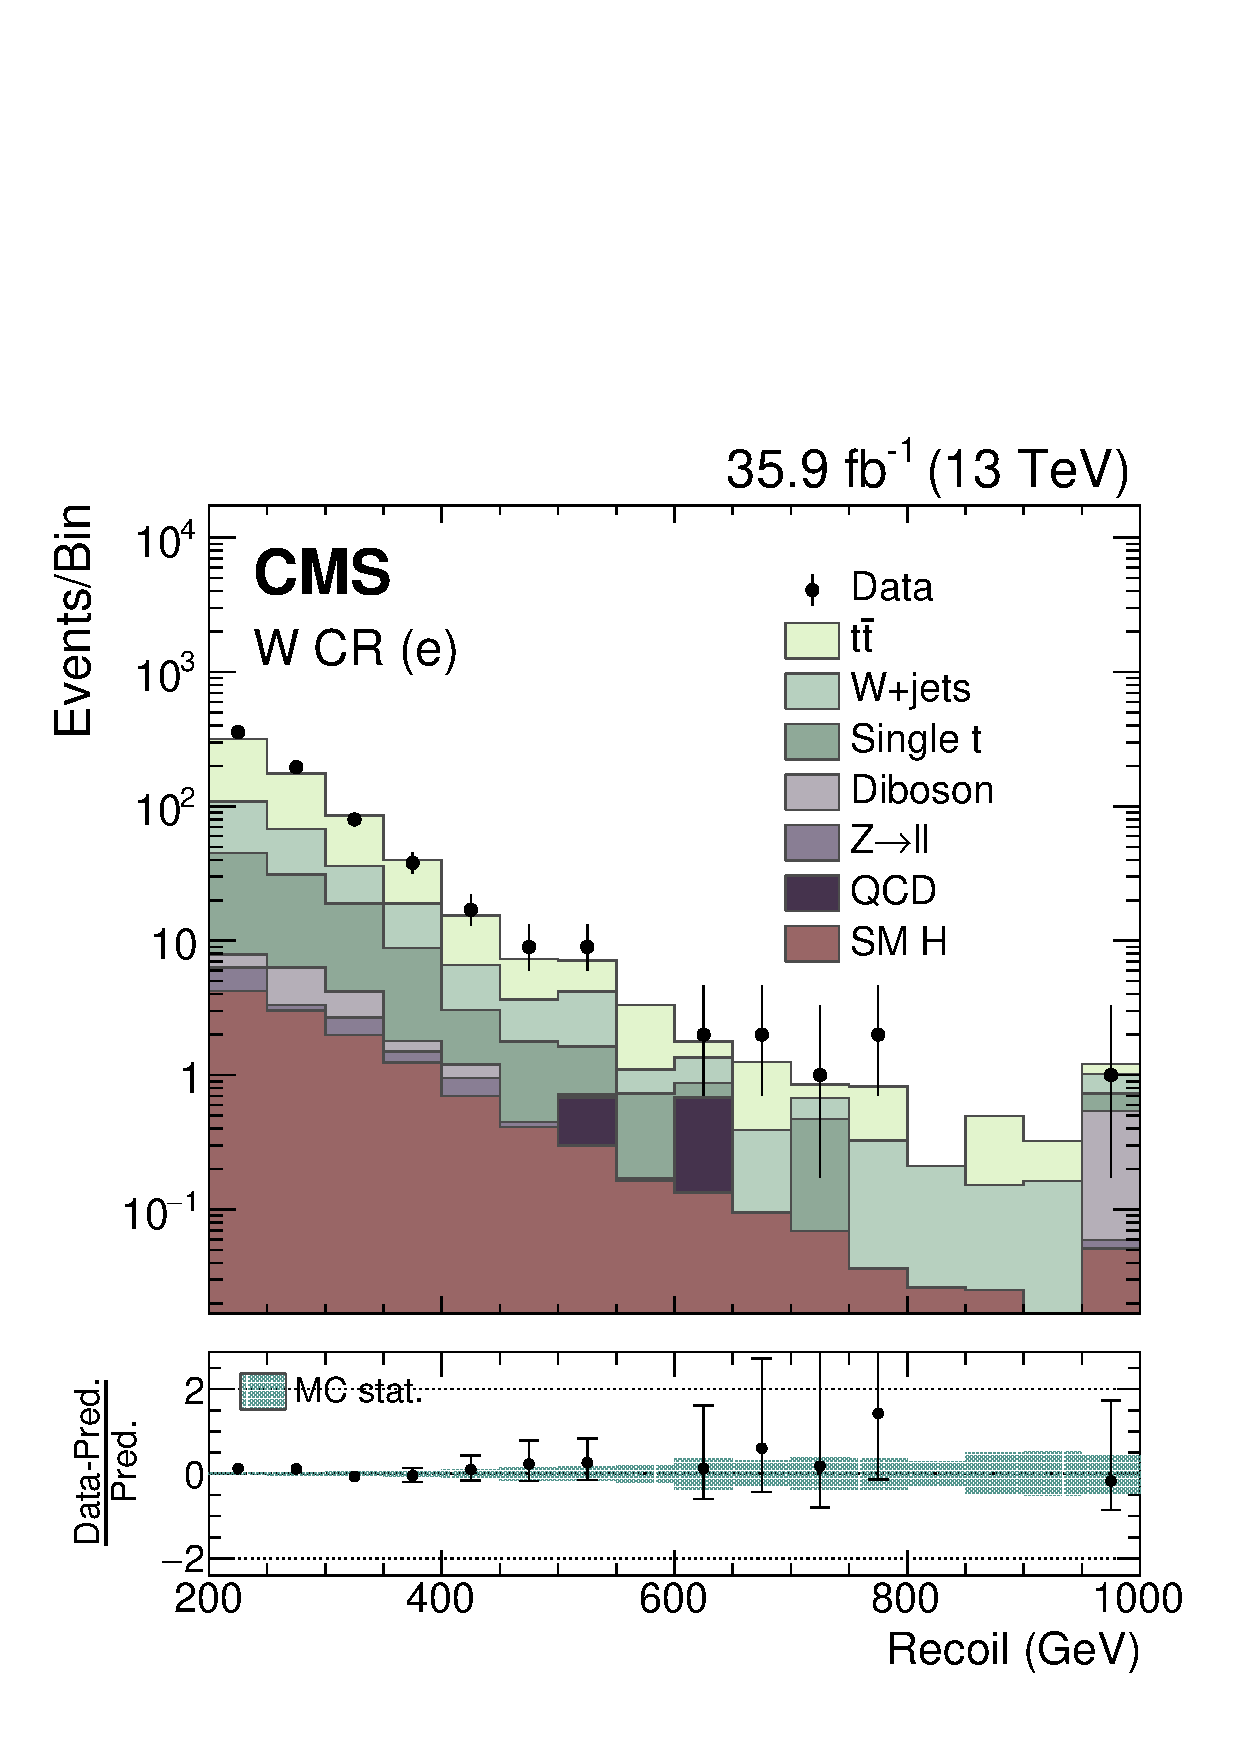
\includegraphics[width=0.4\textwidth]{figures/dataMC/cr_w_el_recoil.pdf}} \\
 \subfloat{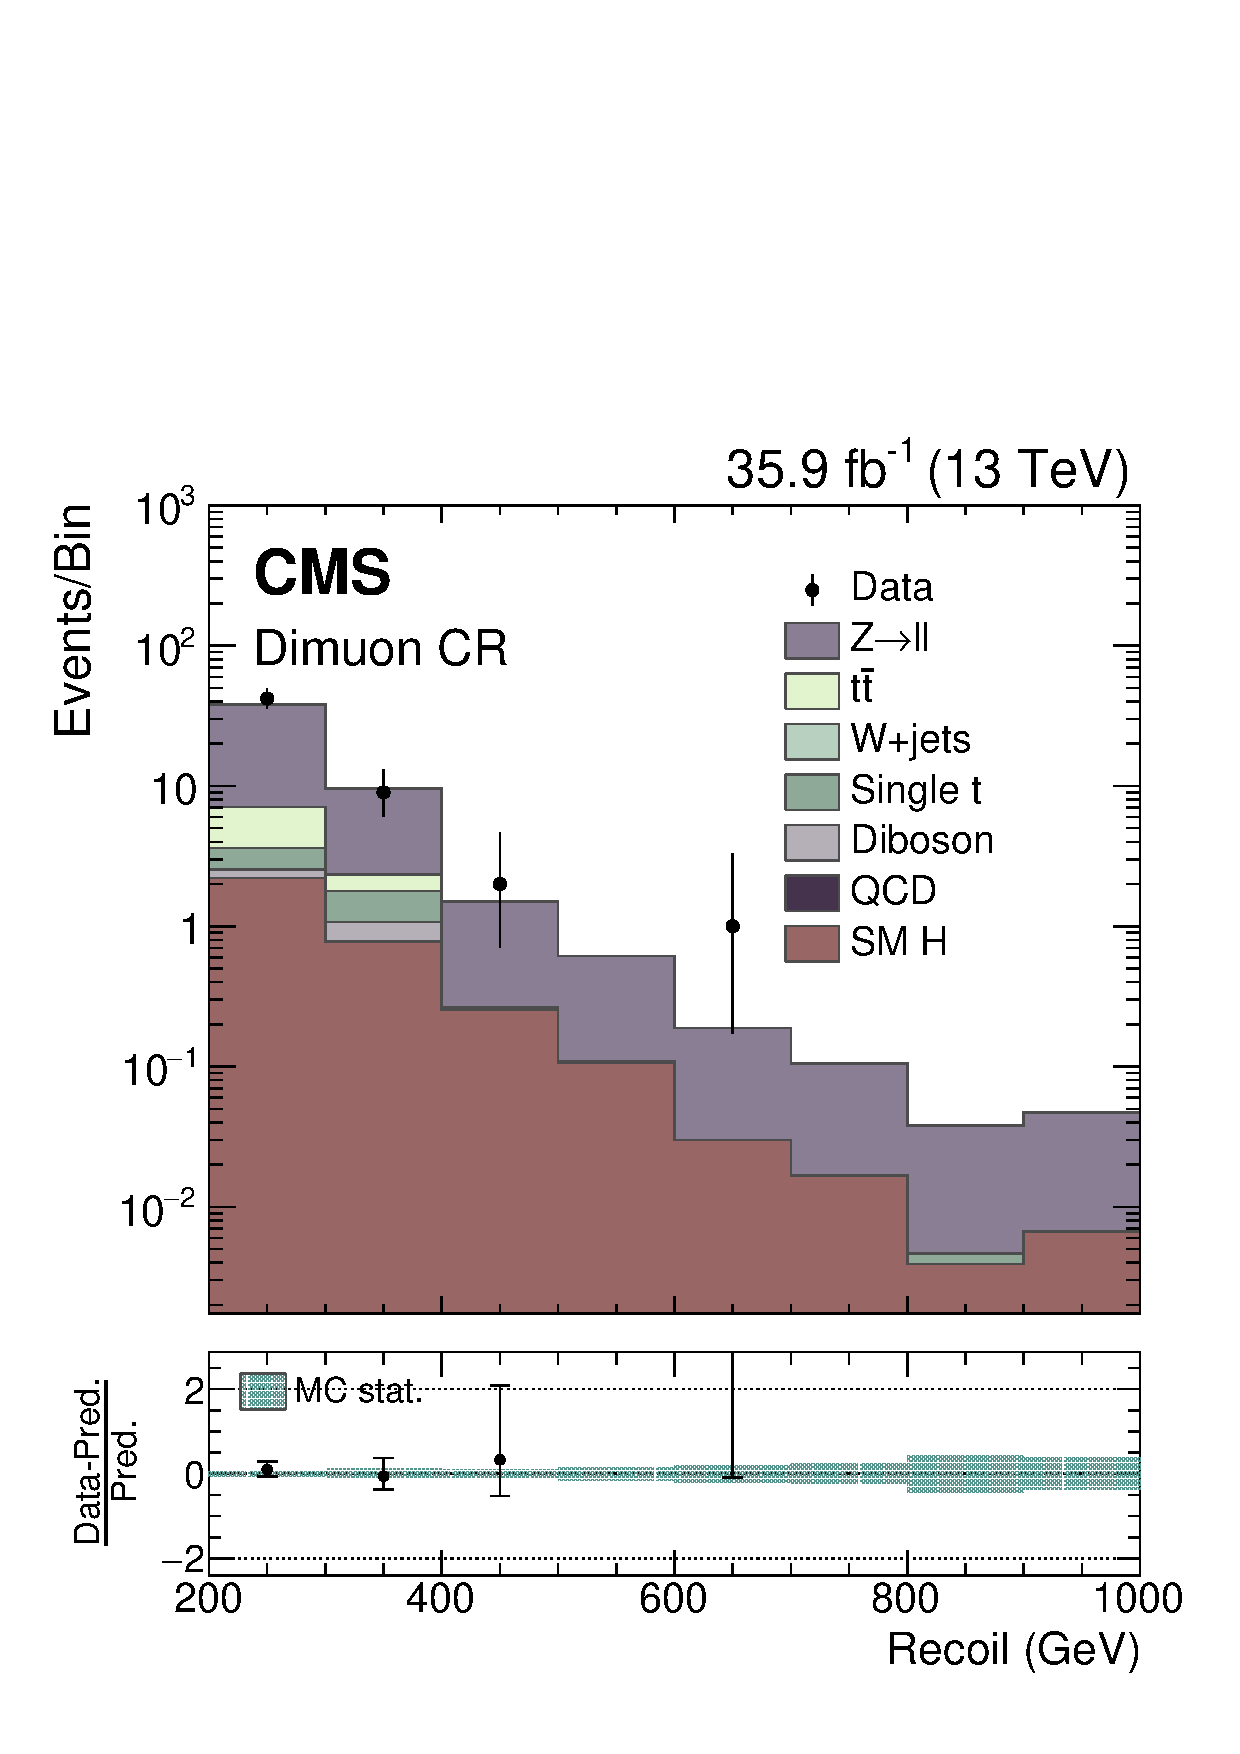
\includegraphics[width=0.4\textwidth]{figures/dataMC/cr_dimuon_recoil.pdf}}
 \subfloat{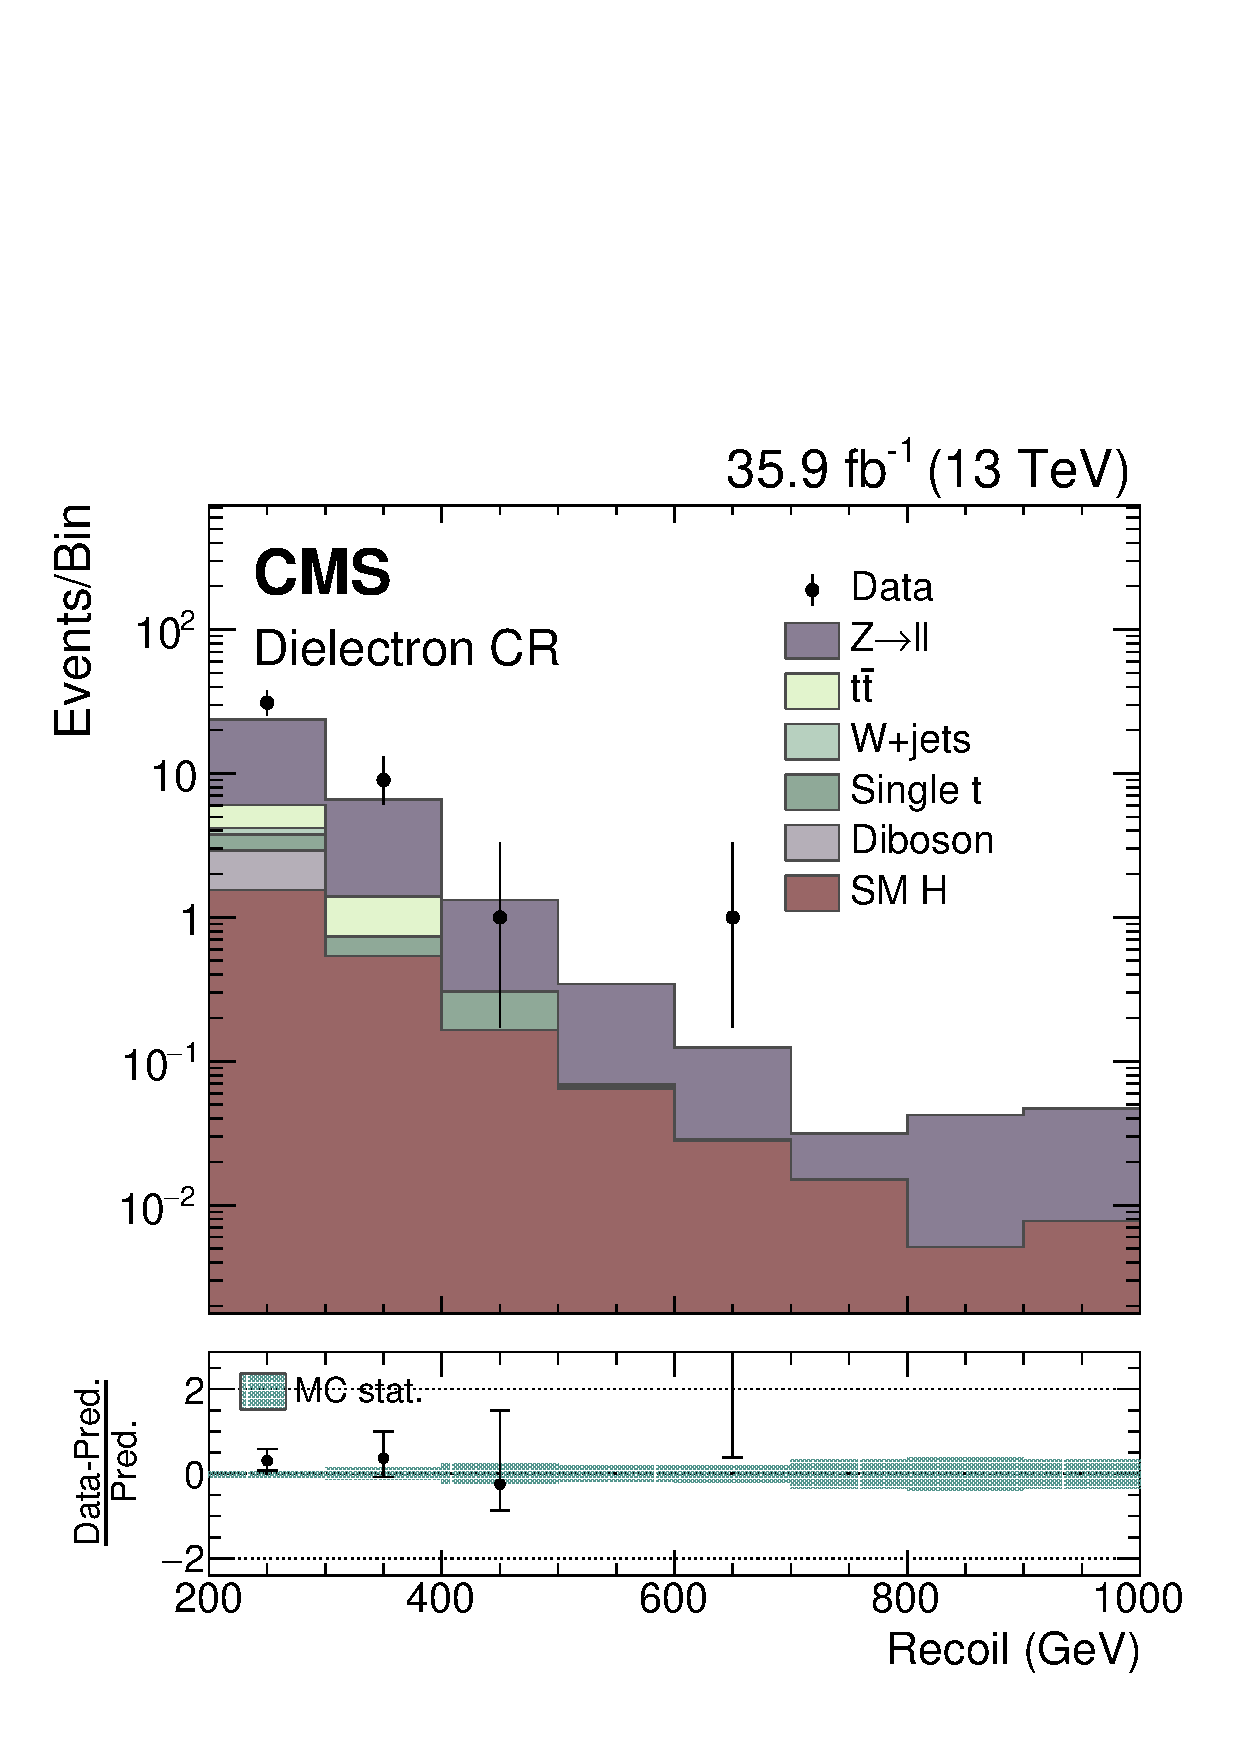
\includegraphics[width=0.4\textwidth]{figures/dataMC/cr_dielectron_recoil.pdf}} \\
\caption{Prefit validation plots in the six CR regions with passing double-b cut, fine binning.}
\label{Fig_cr_Recoil_fine}
\end{figure}




\clearpage


\begin{figure}
\centering
 \subfloat{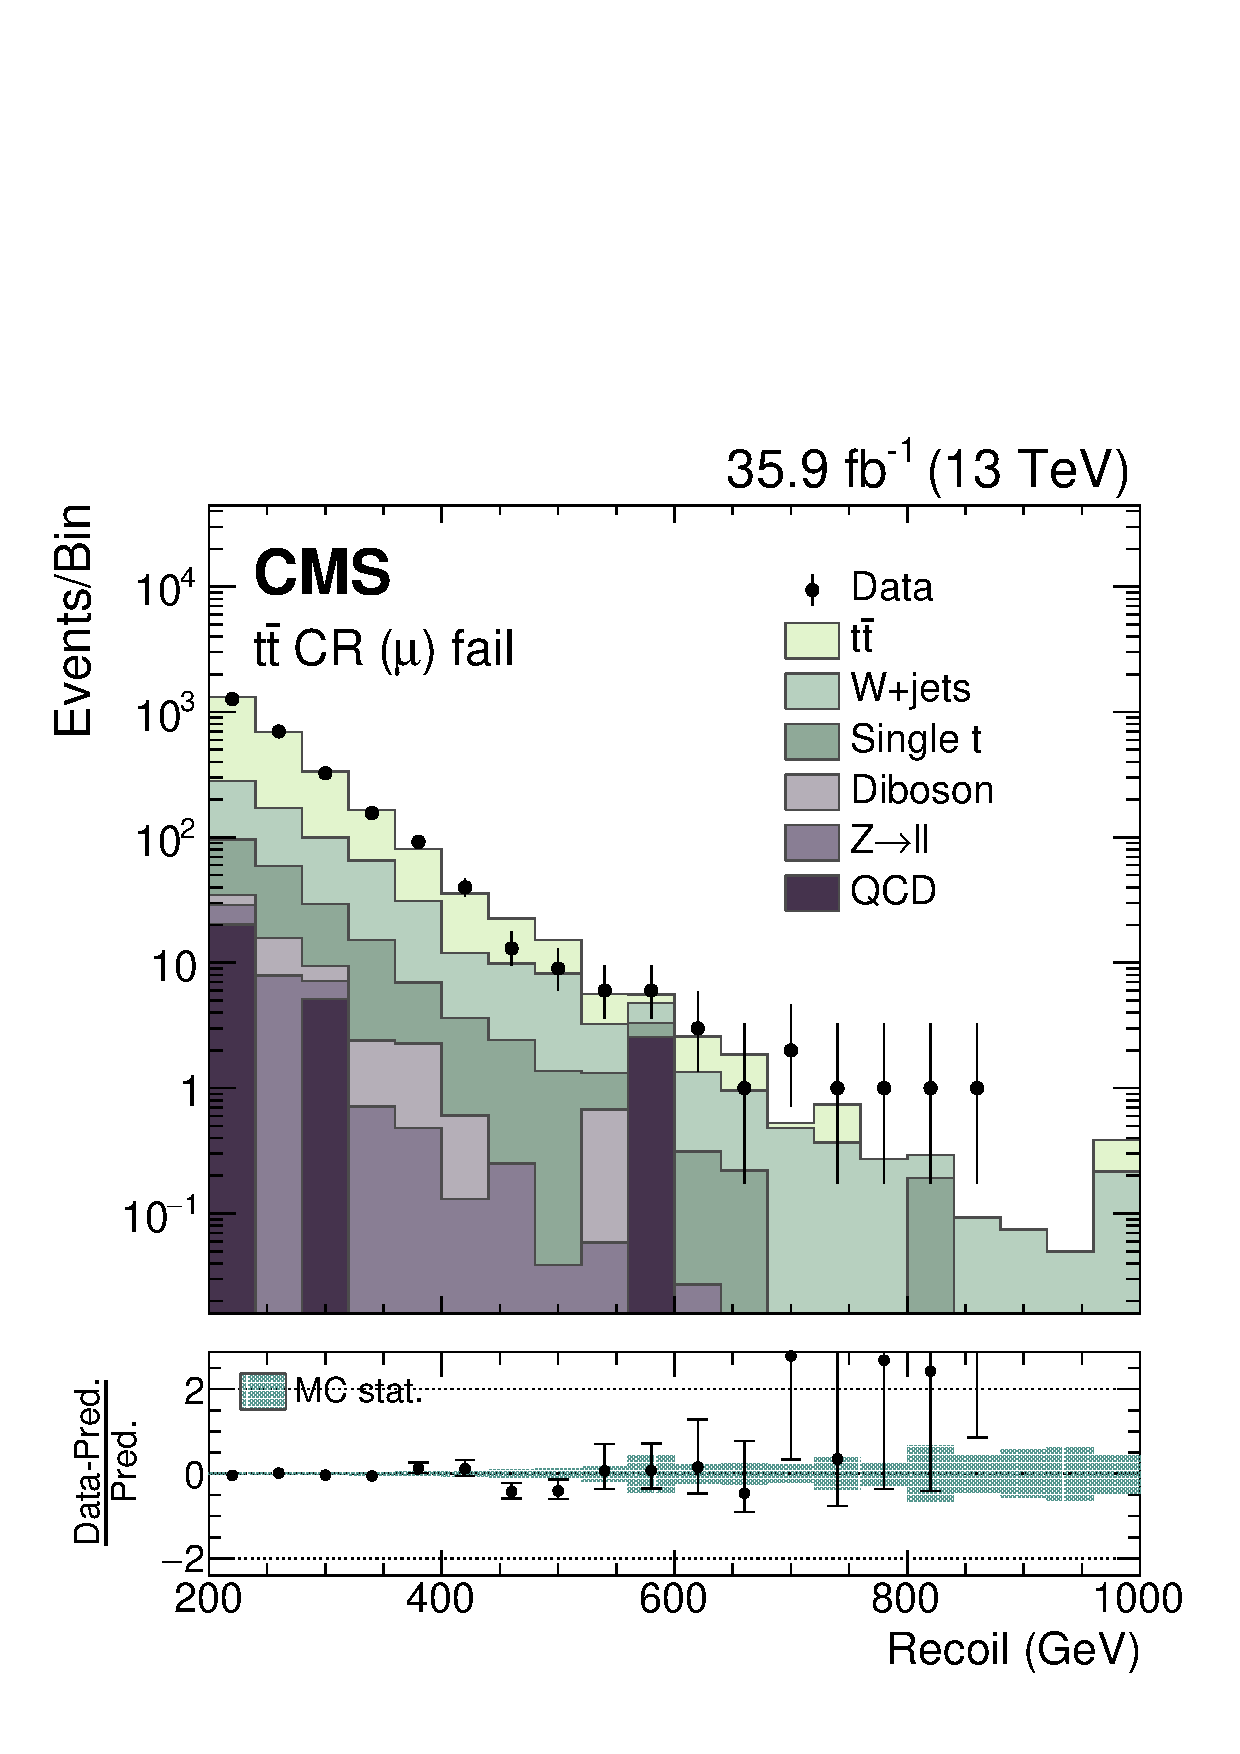
\includegraphics[width=0.4\textwidth]{figures/dataMC/cr_ttbar_mu_fail_recoil.pdf}}
 \subfloat{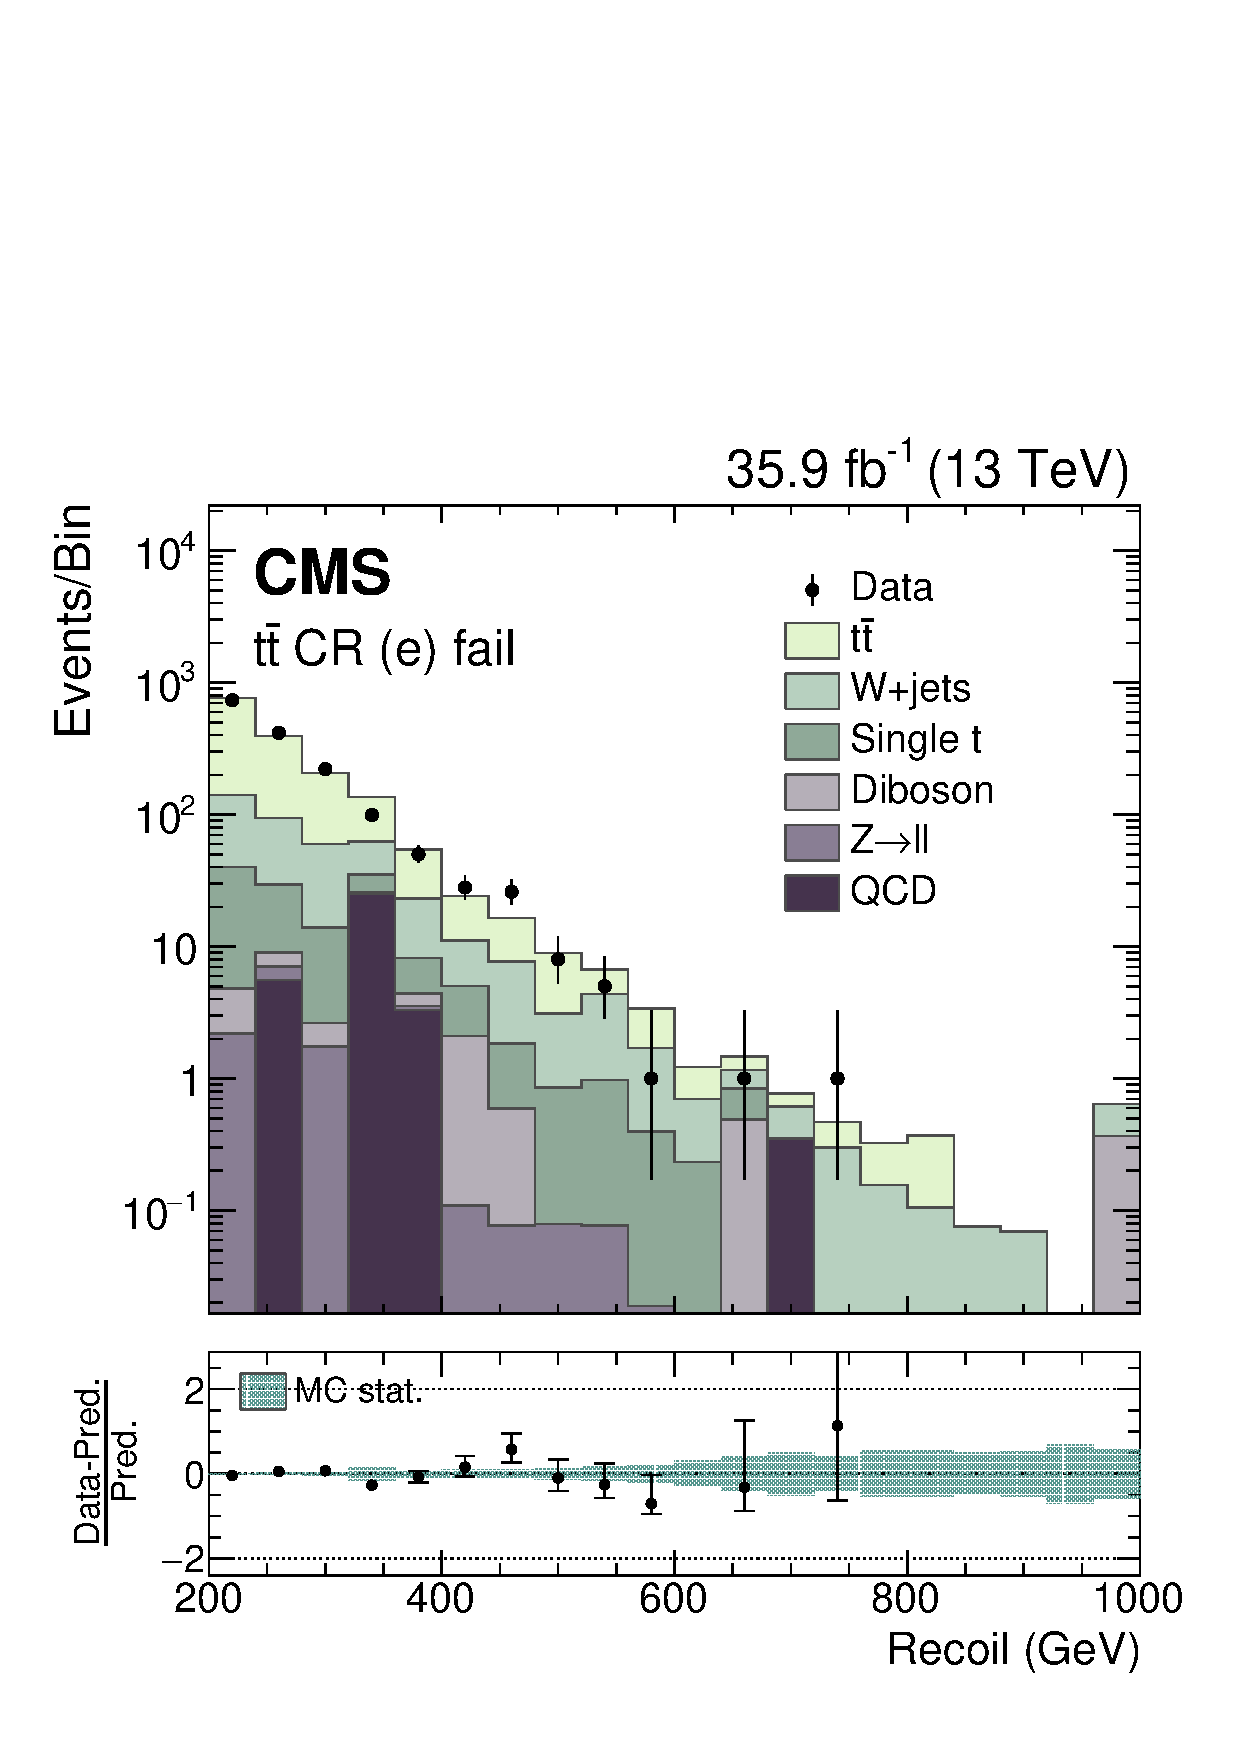
\includegraphics[width=0.4\textwidth]{figures/dataMC/cr_ttbar_el_fail_recoil.pdf}} \\
 \subfloat{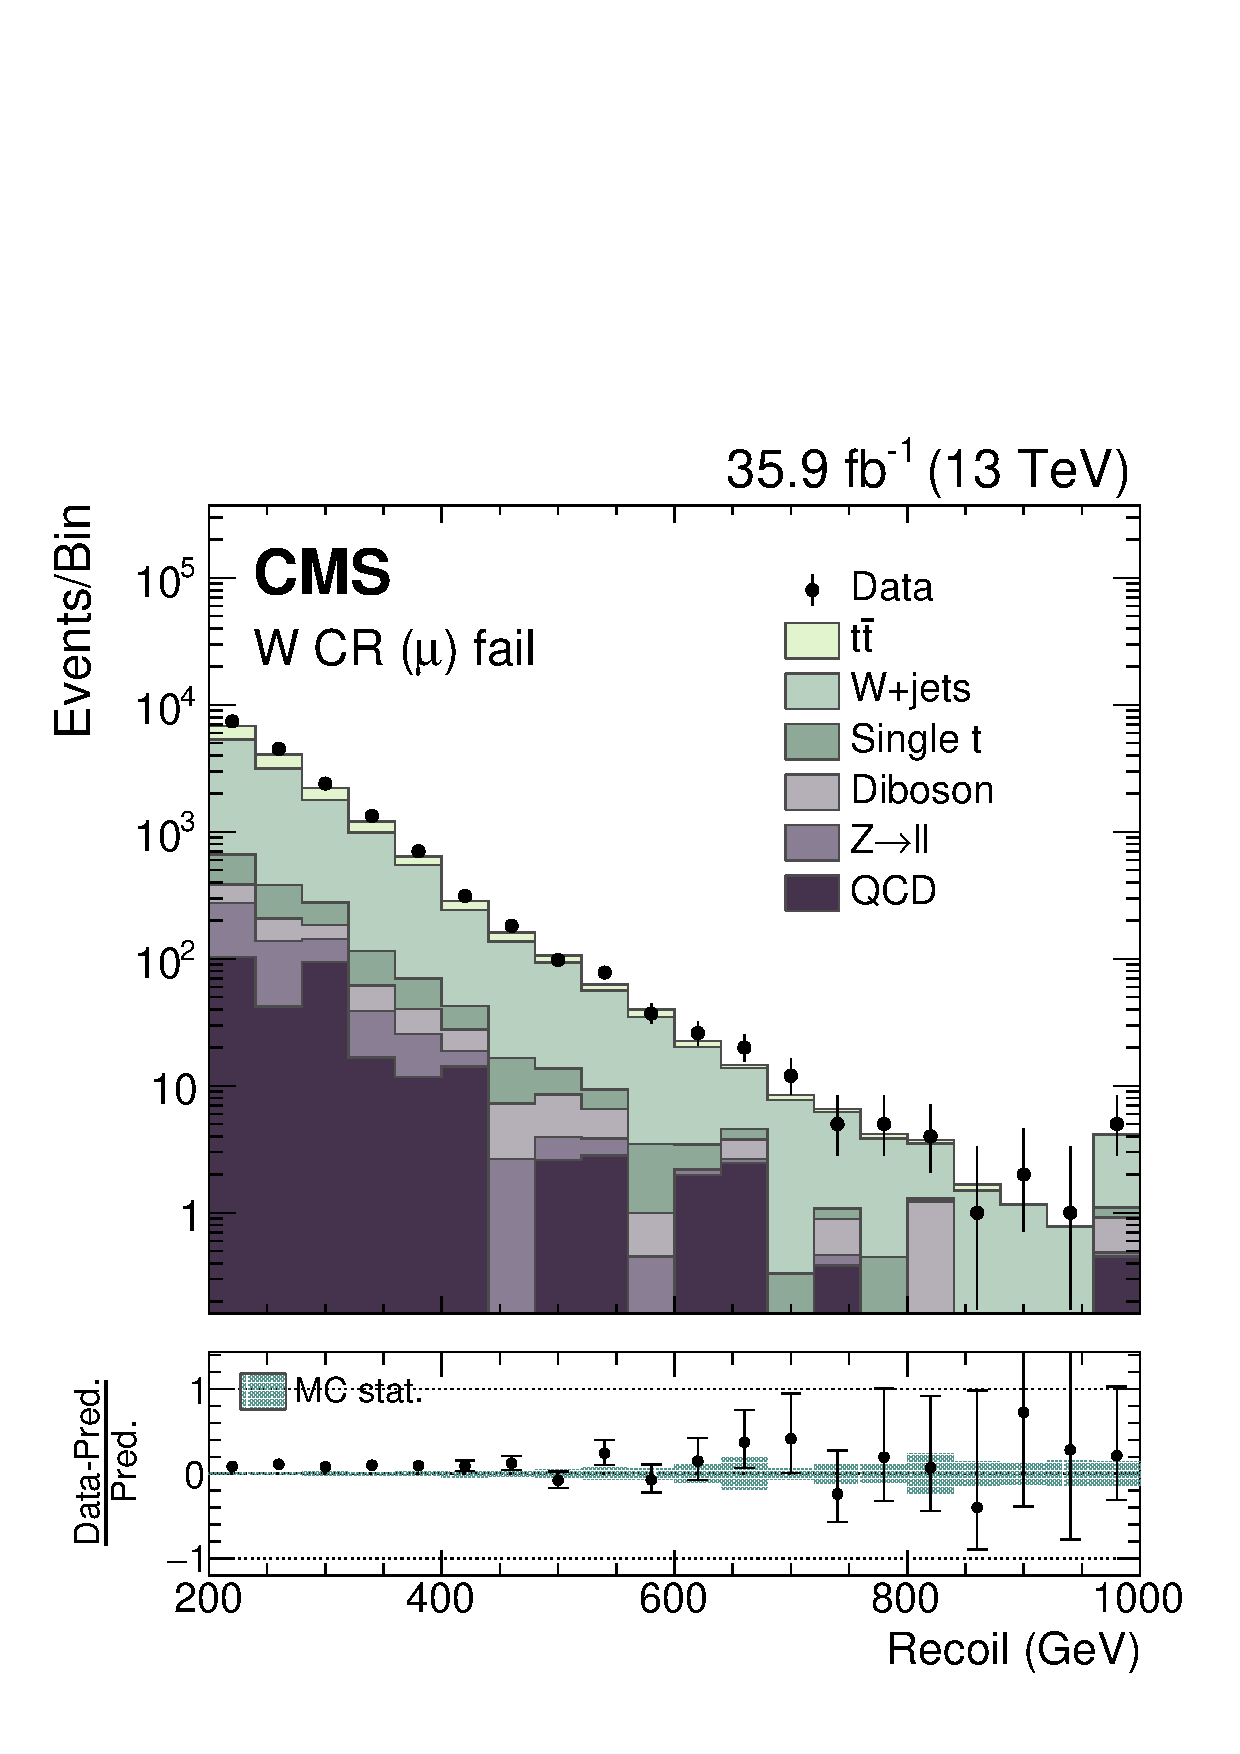
\includegraphics[width=0.4\textwidth]{figures/dataMC/cr_w_mu_fail_recoil.pdf}}
 \subfloat{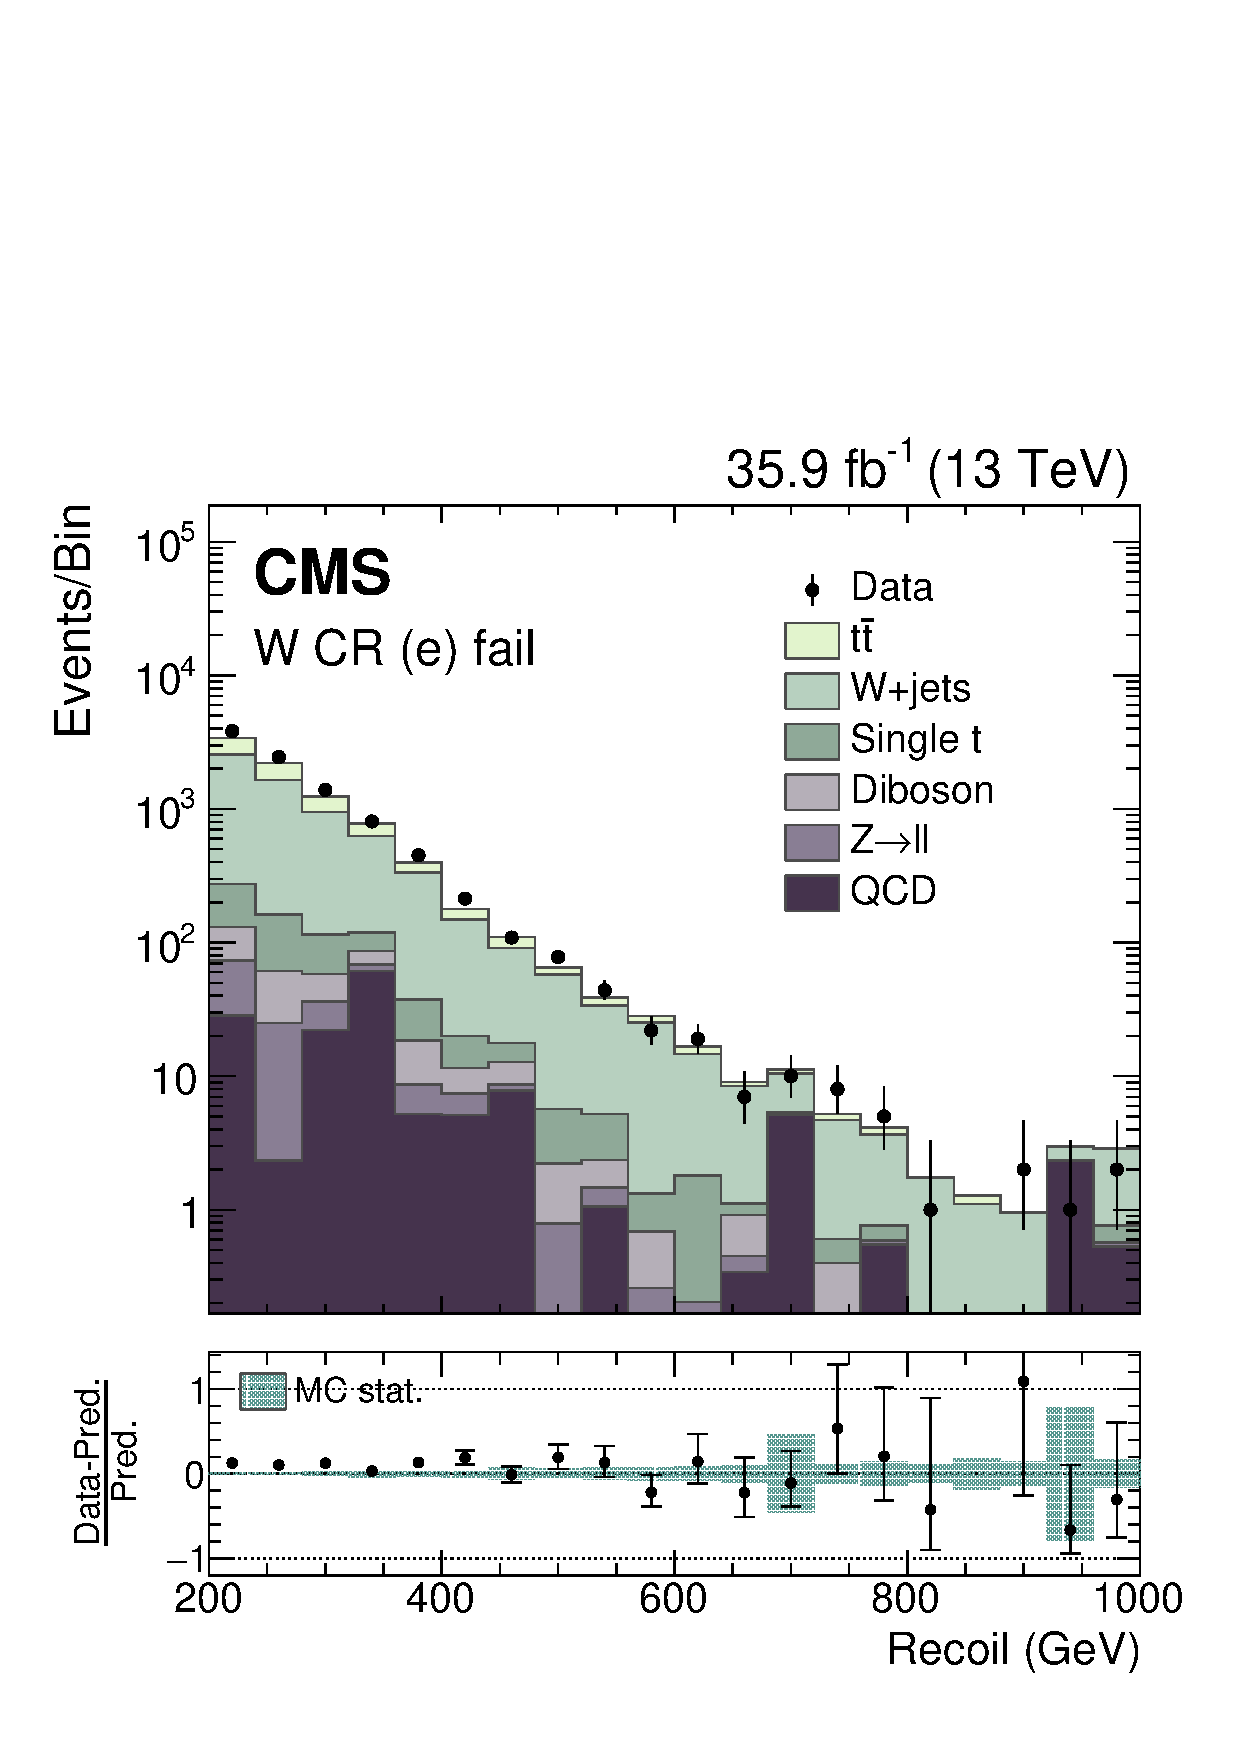
\includegraphics[width=0.4\textwidth]{figures/dataMC/cr_w_el_fail_recoil.pdf}} \\
 \subfloat{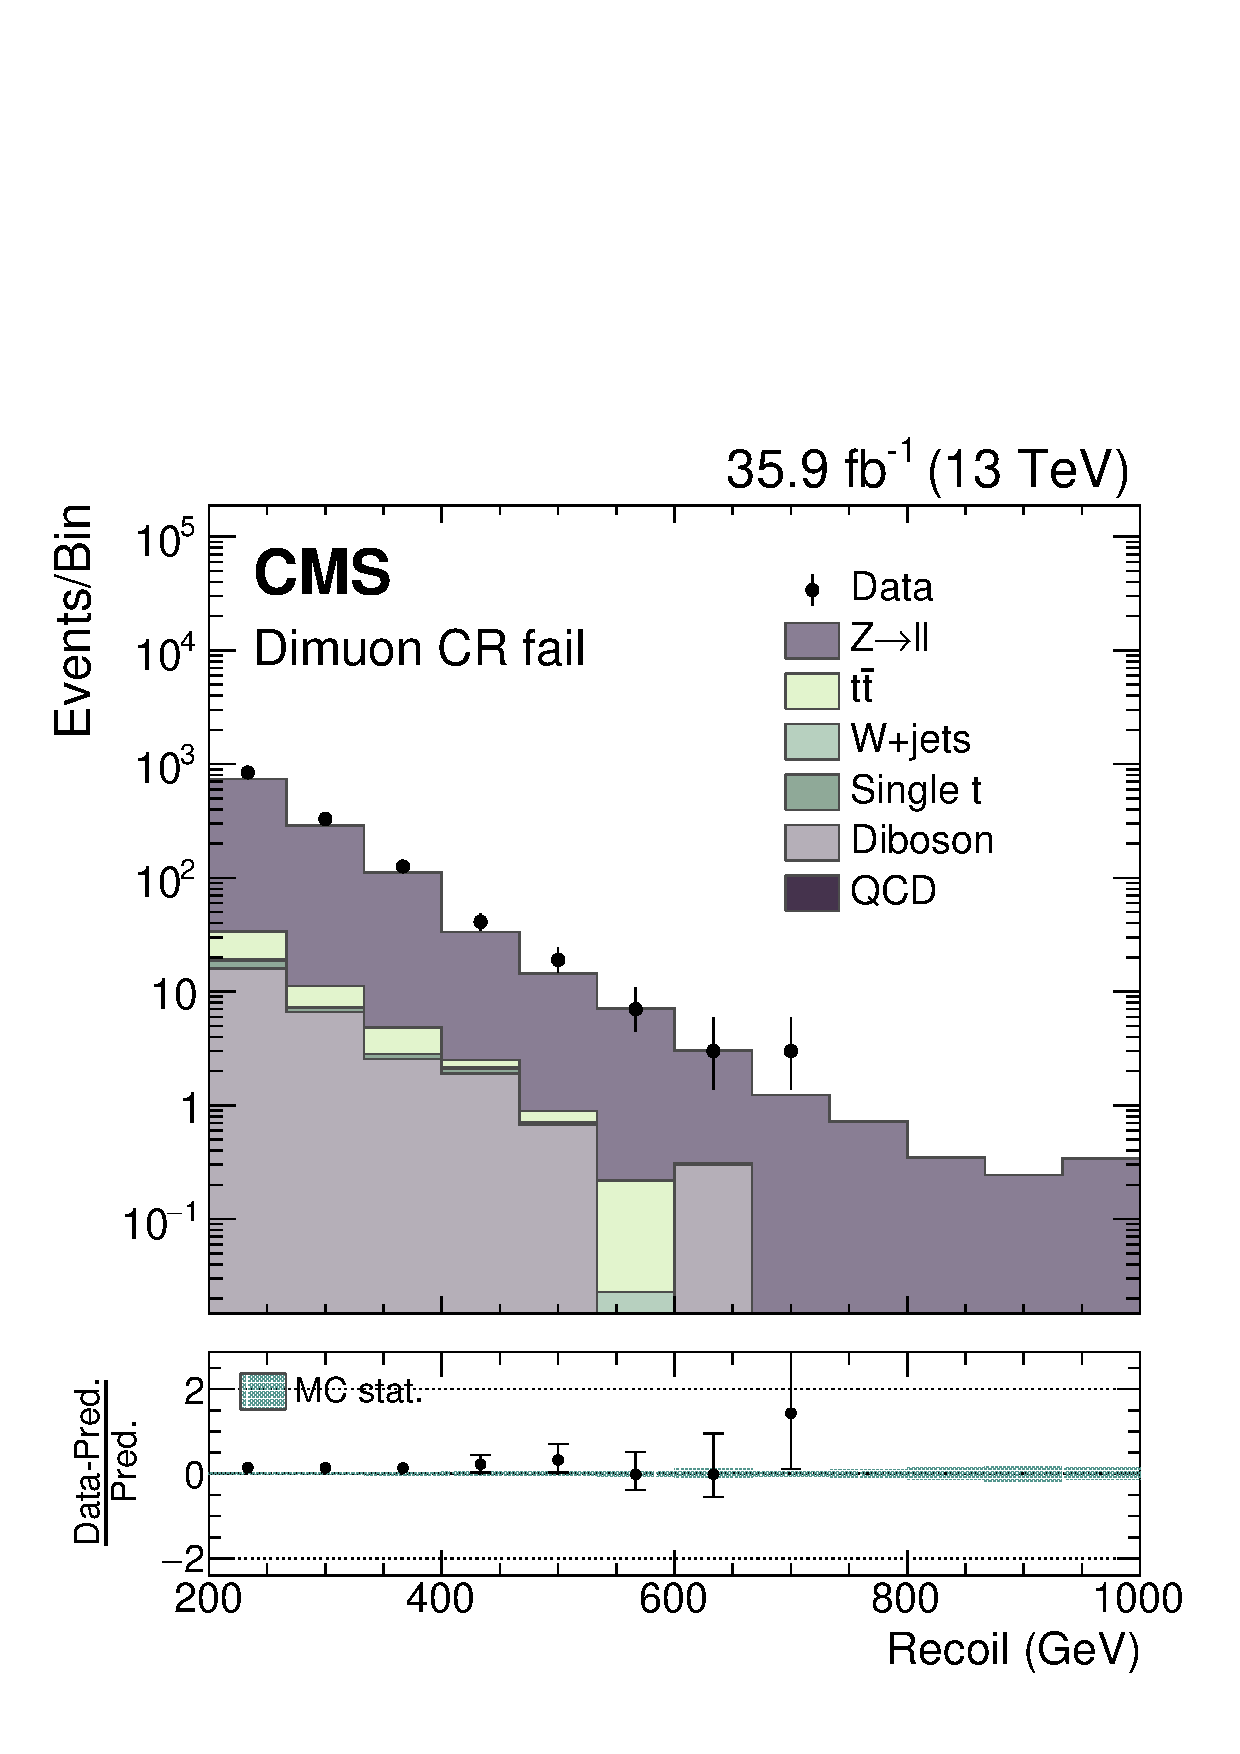
\includegraphics[width=0.4\textwidth]{figures/dataMC/cr_dimuon_fail_recoil.pdf}}
 \subfloat{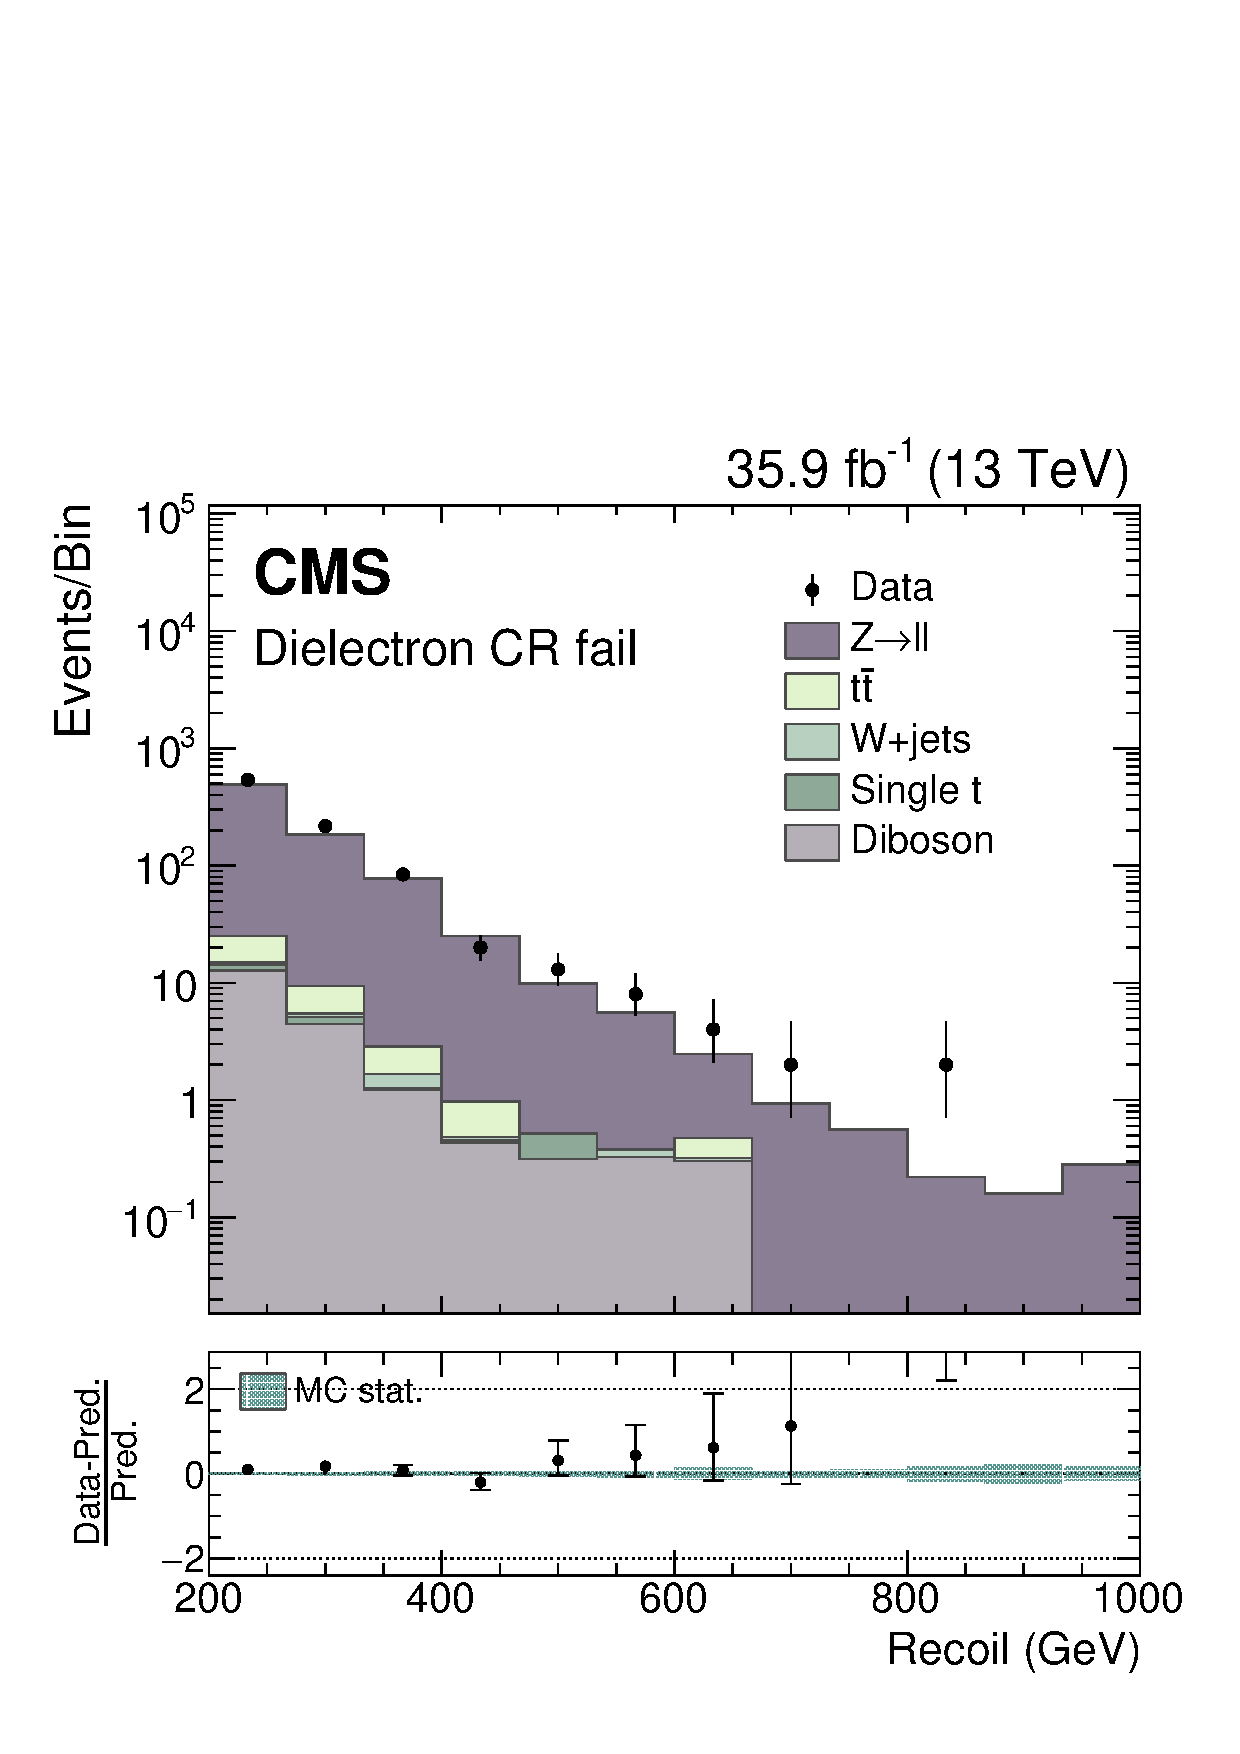
\includegraphics[width=0.4\textwidth]{figures/dataMC/cr_dielectron_fail_recoil.pdf}} \\
\caption{Prefit validation plots in the six CR regions with failing double-b cut, fine binning.}
\label{Fig_cr_Recoil_fail_fine}
\end{figure}


\subsection{Pulls and impacts}

This section of the Appendix shows the plots for the impacts of each systematic uncertainty on the analysis in Figure~\ref{impact}, and the pull distribution of the nuisance parameters for the fit to an Asimov dataset (Figure~\ref{pulls}) and to real data in Figure~\ref{pulls-data}-\ref{pulls-data-signal-masked}. 

\begin{figure}
\centering
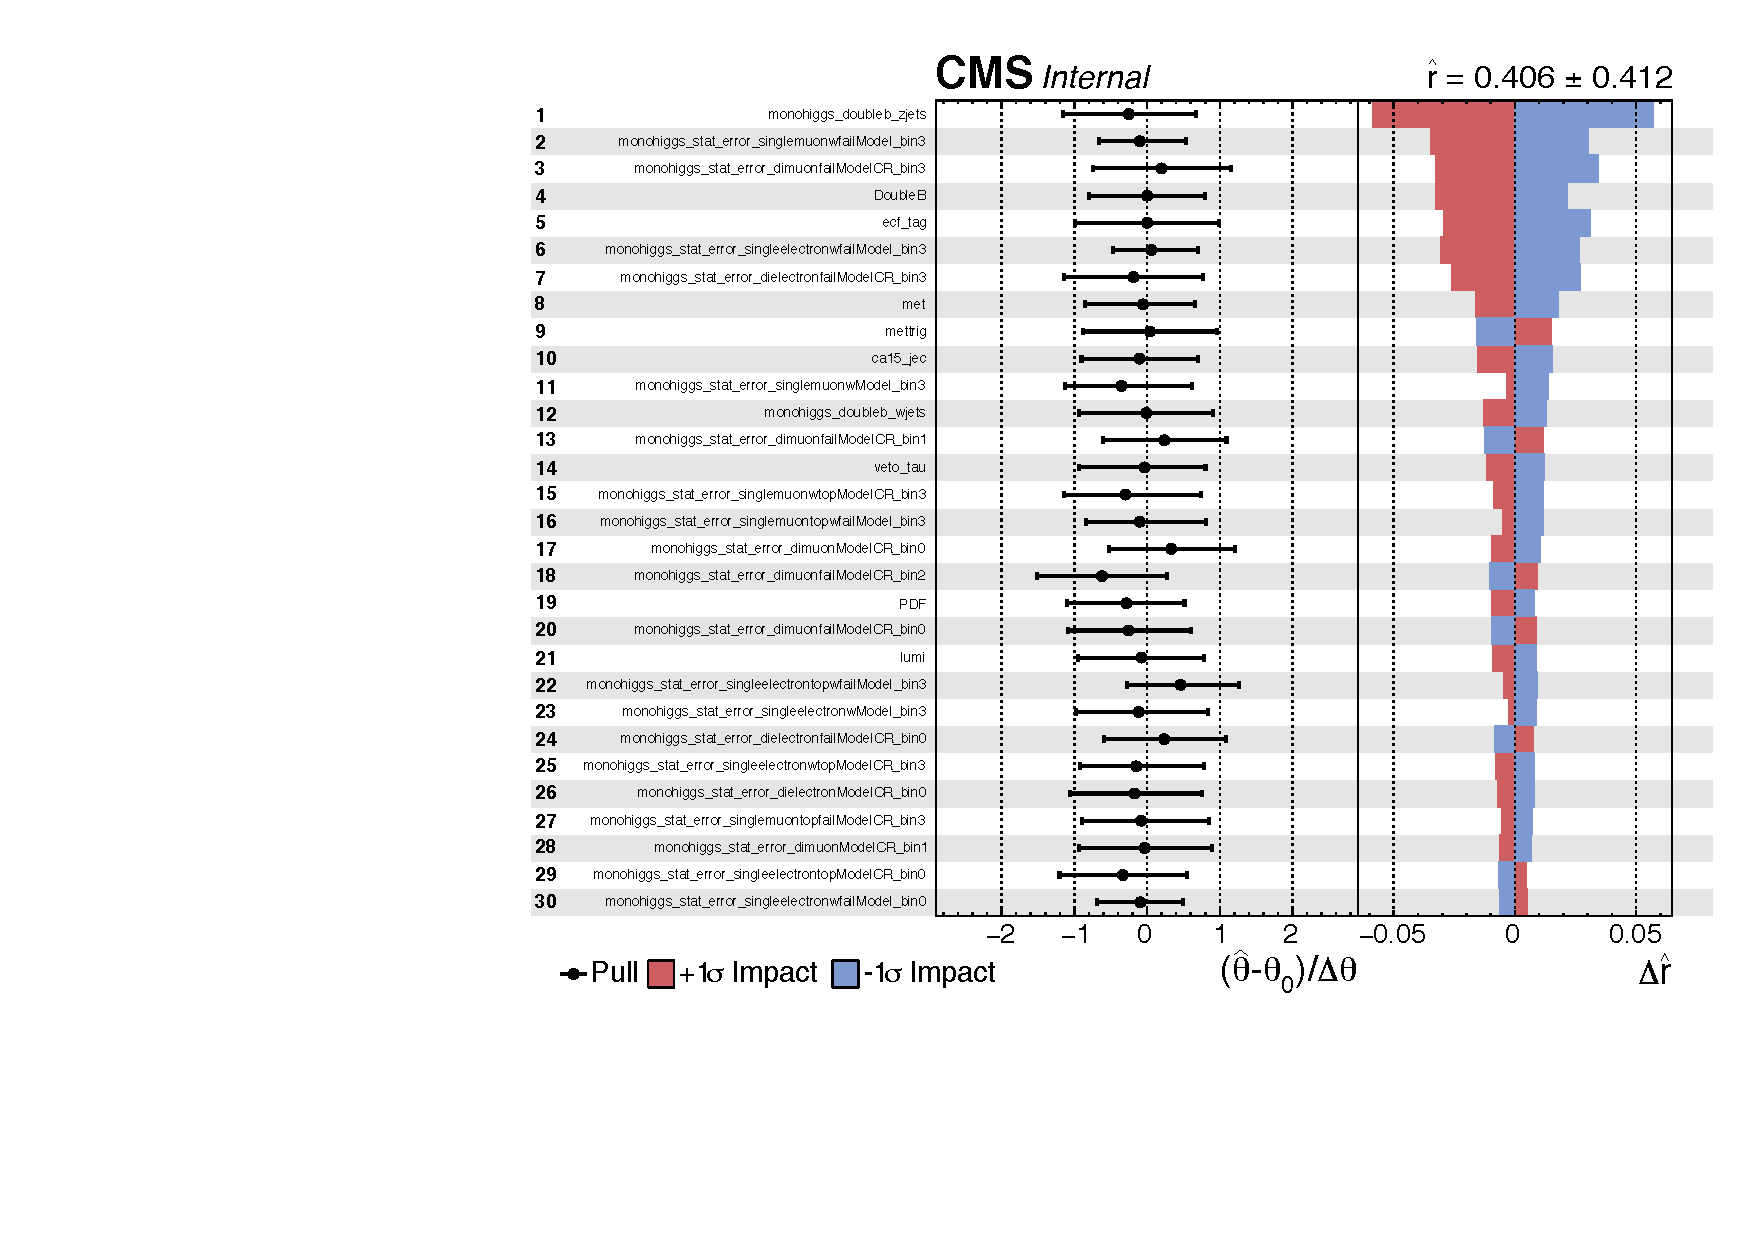
\includegraphics[width=0.95\textwidth]{figures/pullsImpact/impacts_data_1.pdf}
\caption{Impact plot for a fit to data}
\label{impact}
\end{figure}

\clearpage

\begin{figure}
\centering
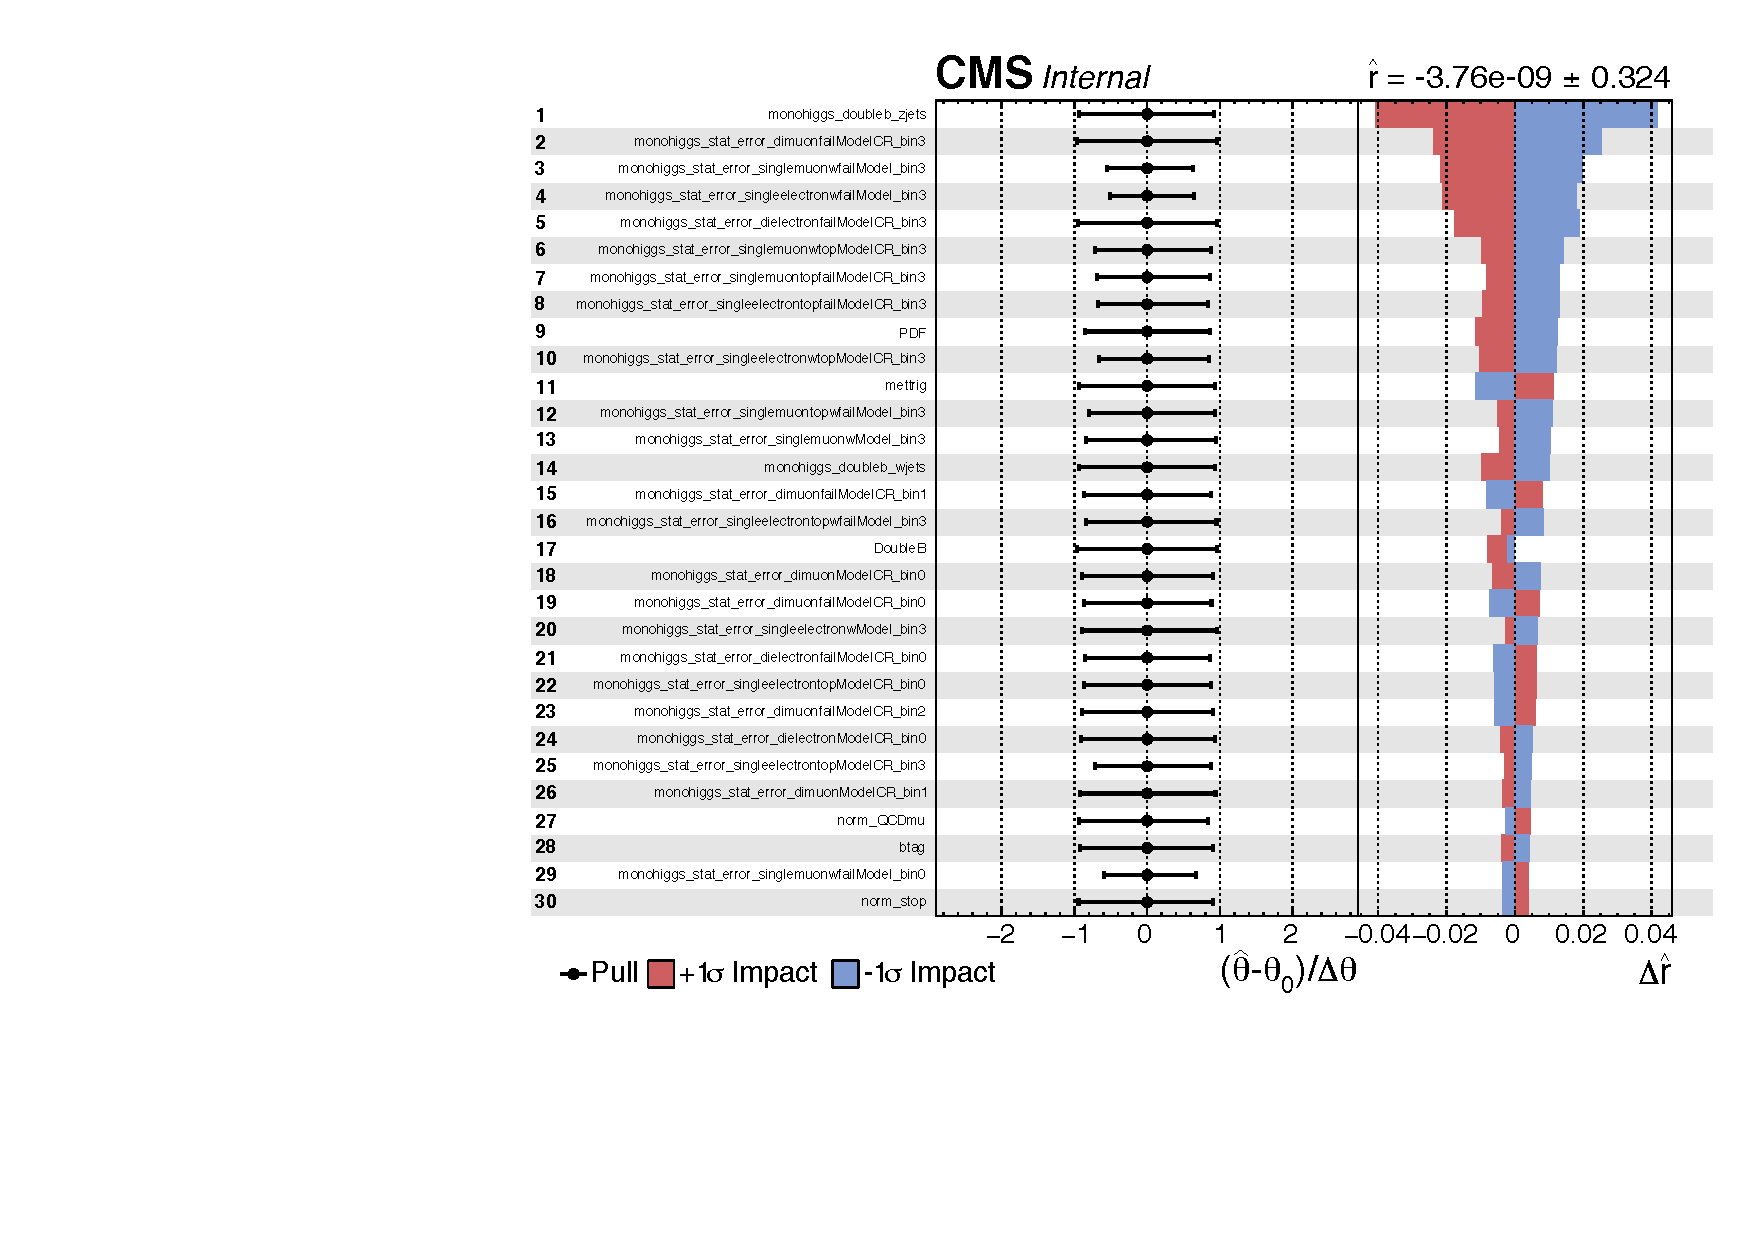
\includegraphics[width=0.95\textwidth]{figures/pullsImpact/impacts_asimov_1.pdf}
\caption{Impact plot for a fit to an Asimov data set}
\label{impact2}
\end{figure}

\clearpage


\begin{figure}
\centering
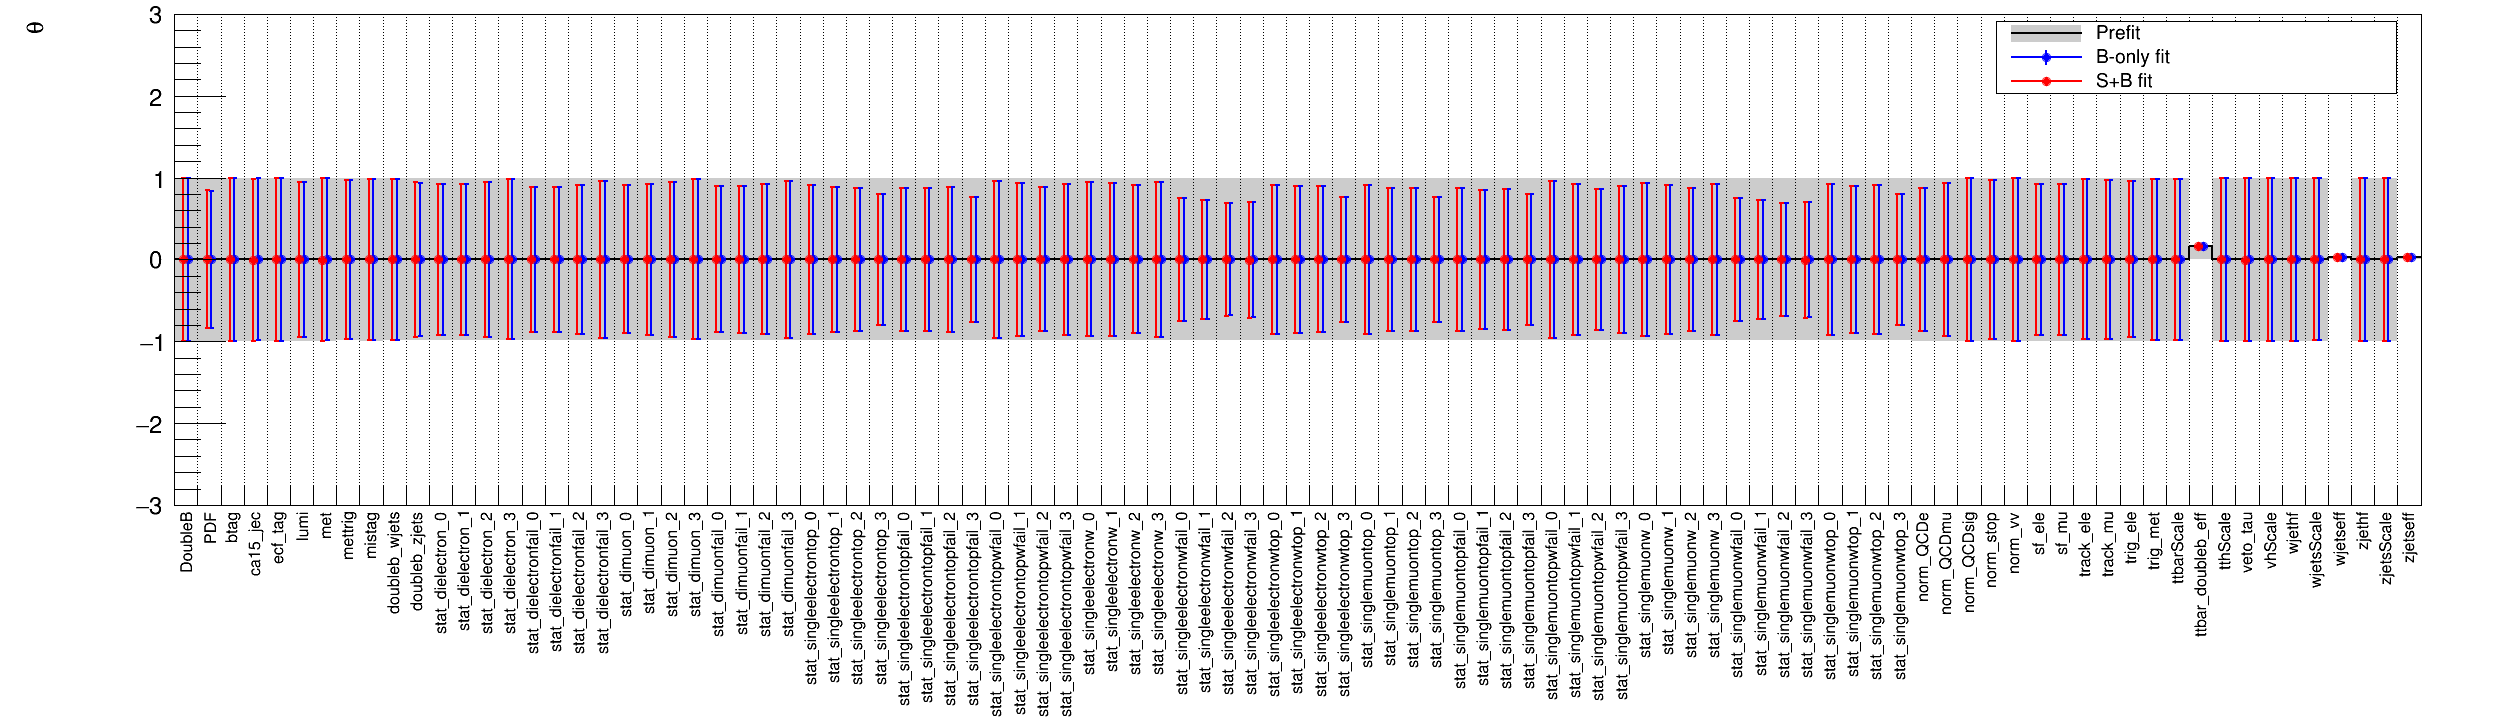
\includegraphics[width=1.25\textwidth, angle =90]{figures/pullsImpact/pulls_asimov.png}\\
\caption{Pulls distribution for Asimov data.}
\label{pulls}
\end{figure}


\clearpage


\begin{figure}
\centering
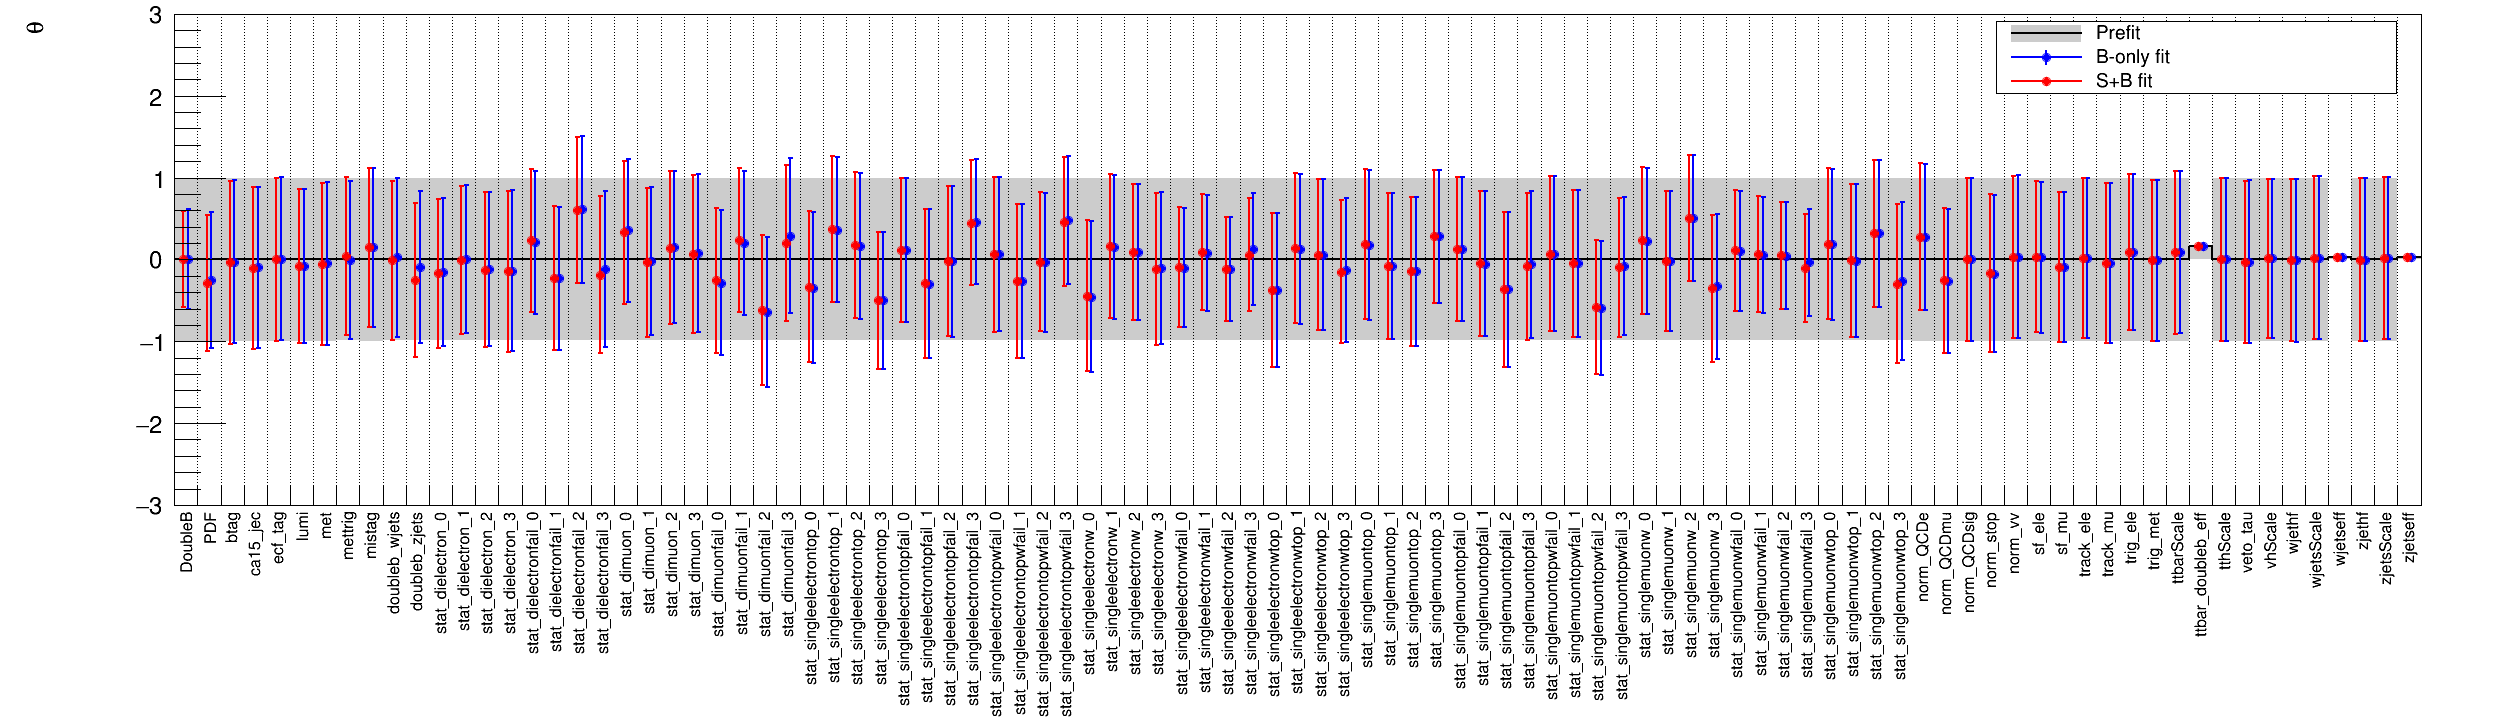
\includegraphics[width=1.25\textwidth, angle =90]{figures/pullsImpact/pulls_data.png}
\caption{Pulls distribution for the data. }
\label{pulls-data}
\end{figure}

\clearpage


\begin{figure}
\centering
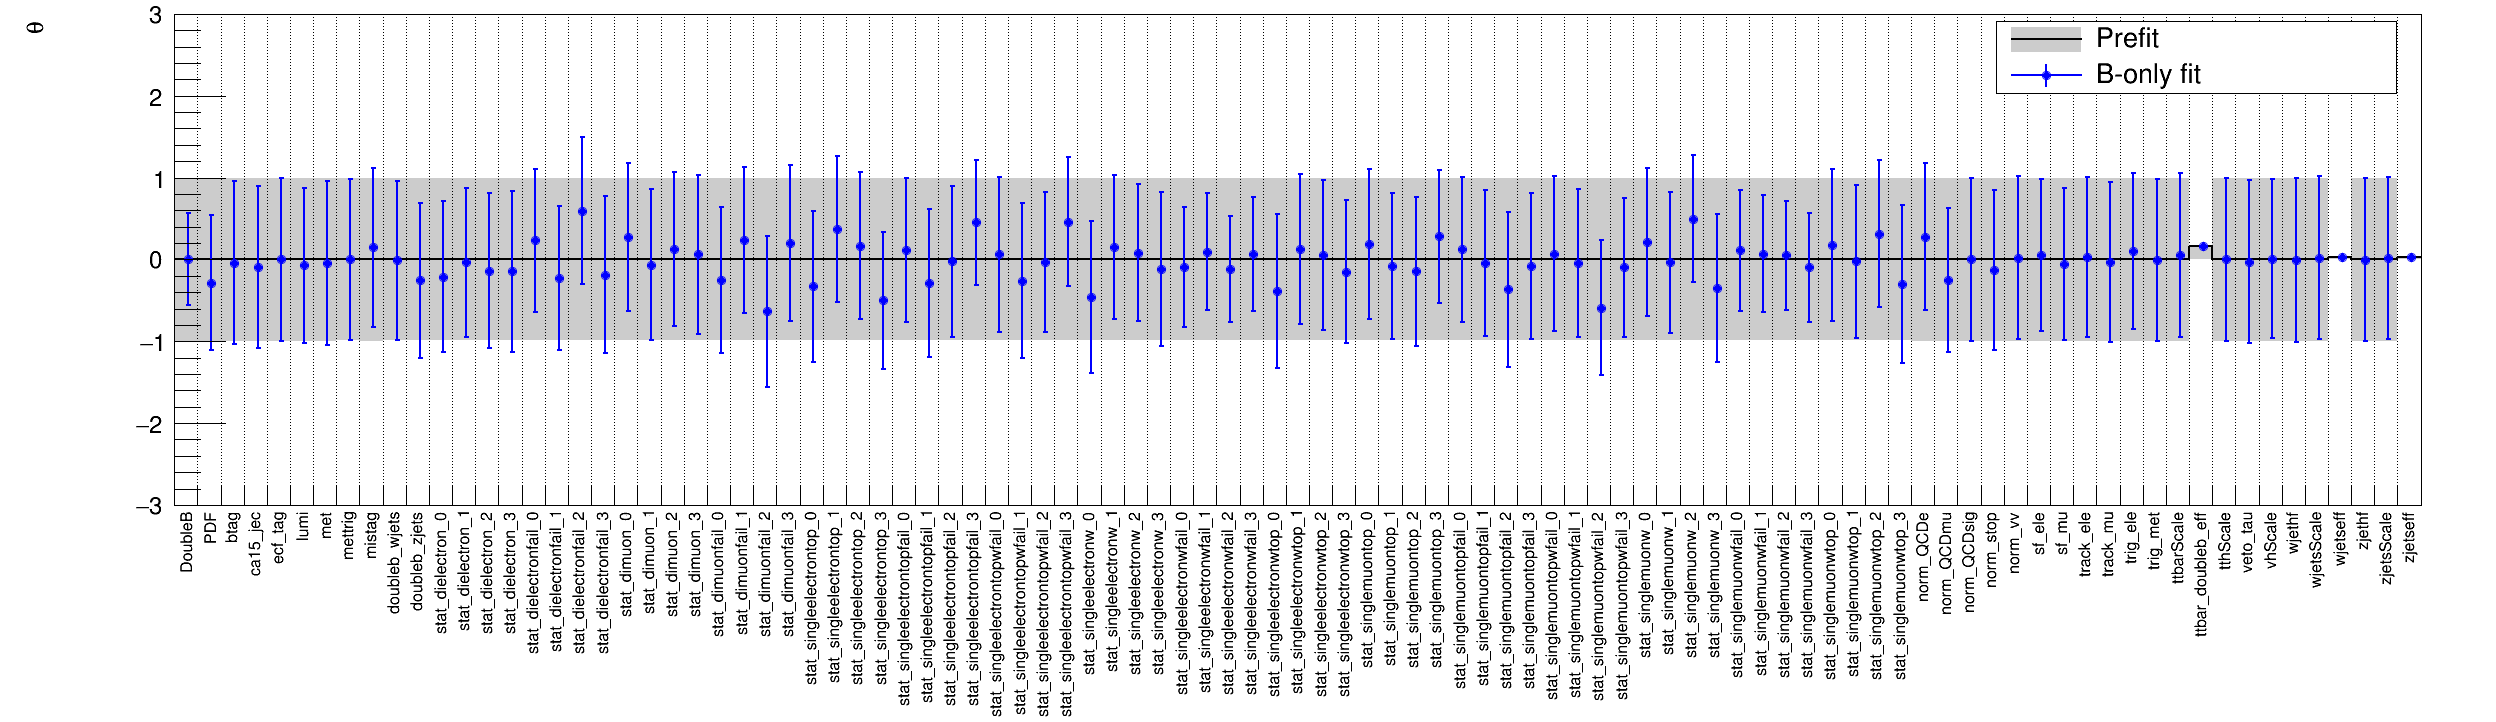
\includegraphics[width=1.25\textwidth, angle =90]{figures/pullsImpact/pulls_data_maskedsignal.png}
\caption{Pulls distribution for the data for a CR-only fit.}
\label{pulls-data-signal-masked}
\end{figure}


\clearpage


\begin{figure}
\centering
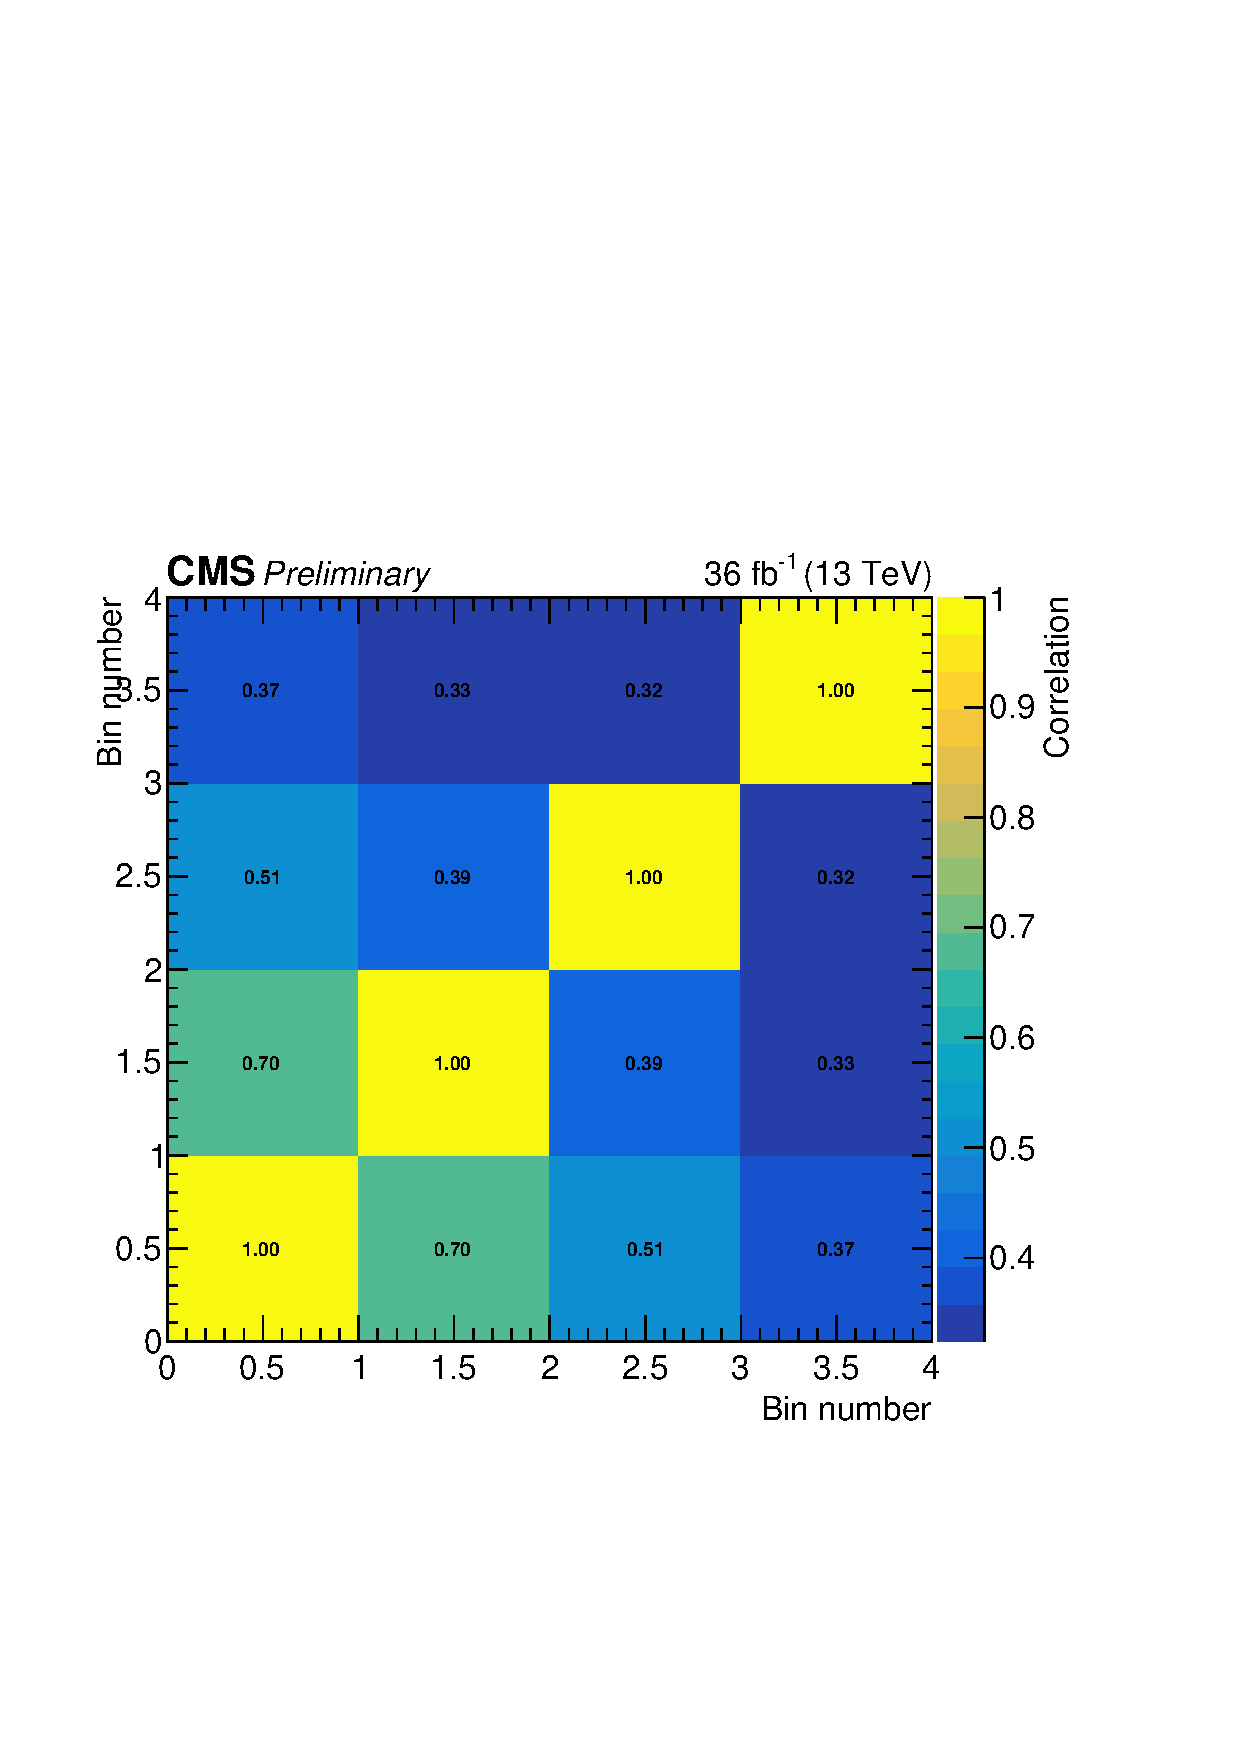
\includegraphics[width=0.65\textwidth]{figures/pullsImpact/corr.pdf}
\caption{Correlations between the uncertainties in the estimated background yields in all the \ETmiss bins of the signal region. Bin1: 200-270\,GeV. Bin2: 270-350\,GeV. Bin3: 350-475\,GeV. Bin4: $>475$\,GeV.}
\label{covariance_matrix}
\end{figure}

\clearpage

\begin{figure}
\centering
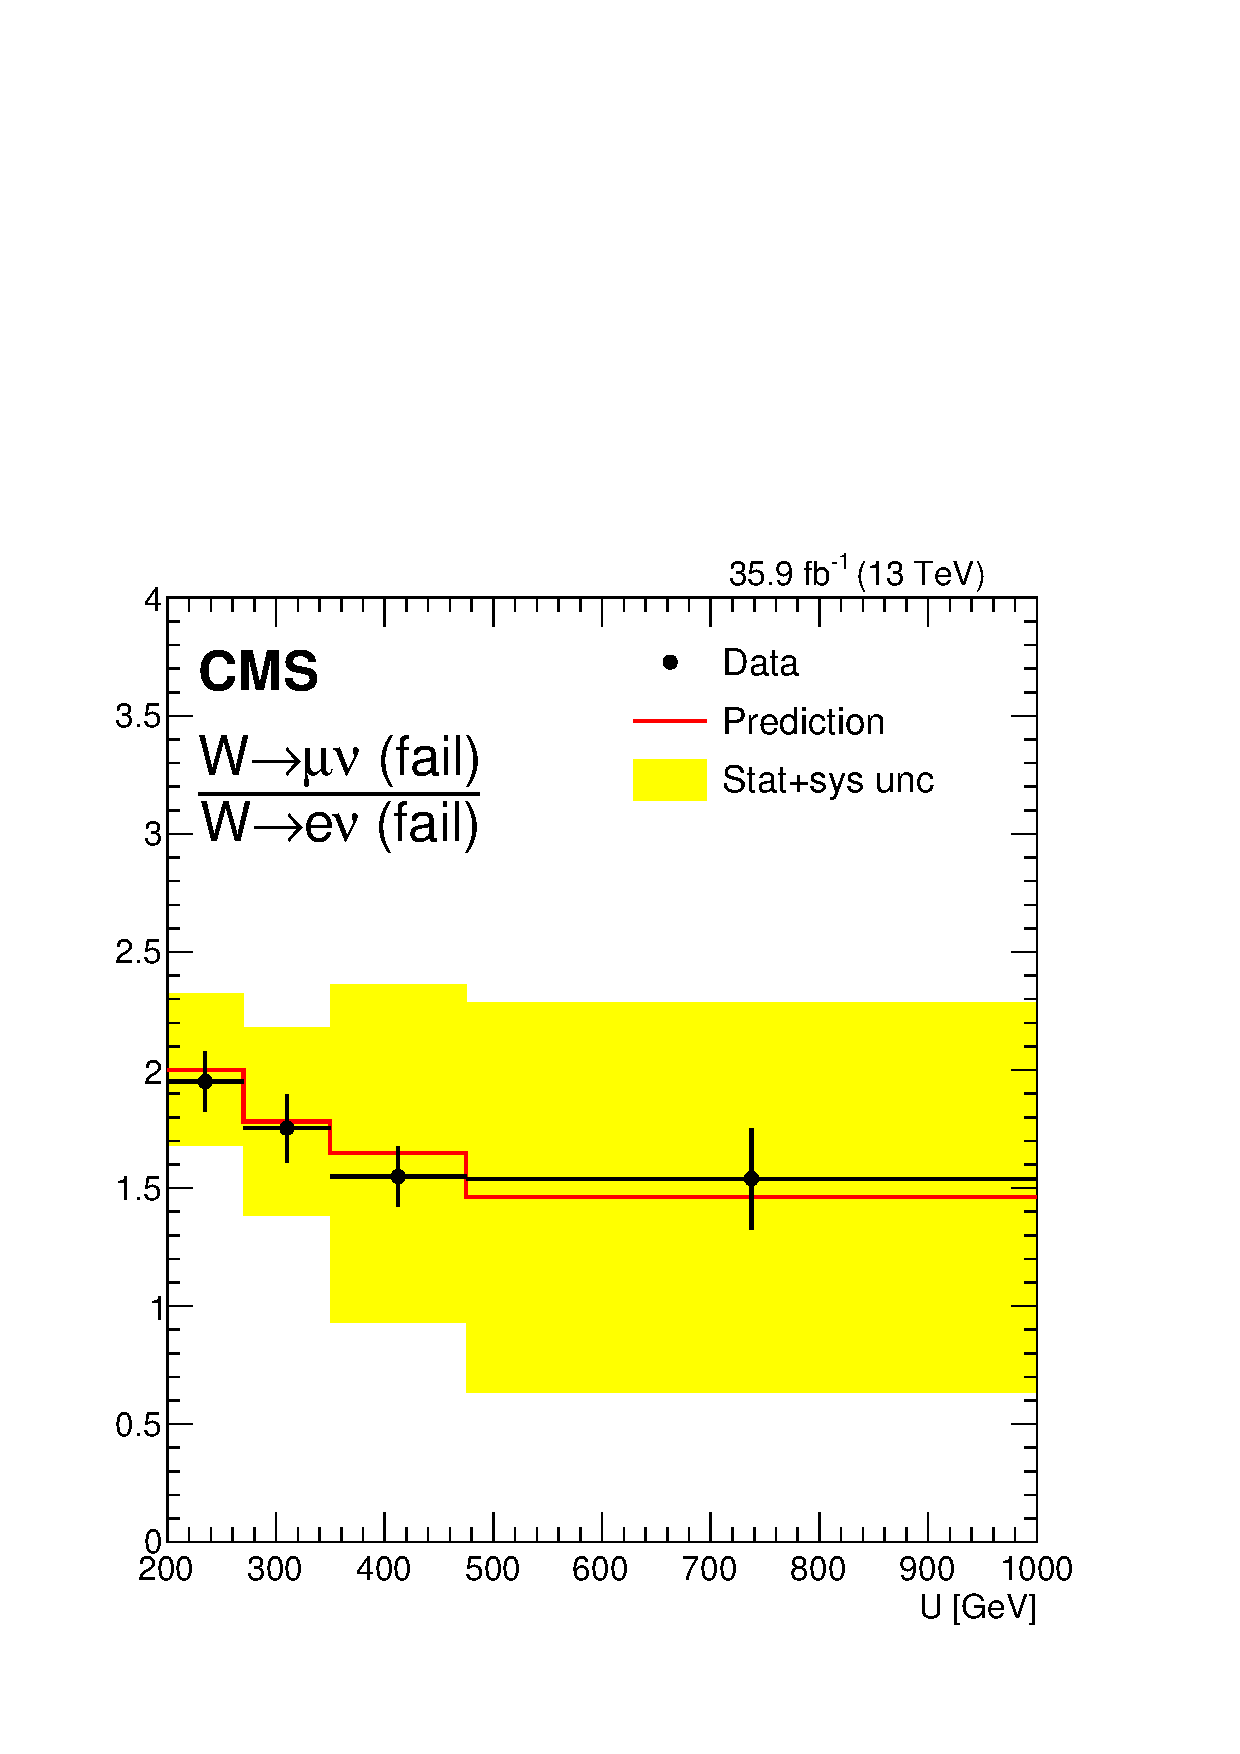
\includegraphics[width=0.45\textwidth]{figures/pullsImpact/ratio_wmn_fail_wen_fail_shapes_prefit.pdf}
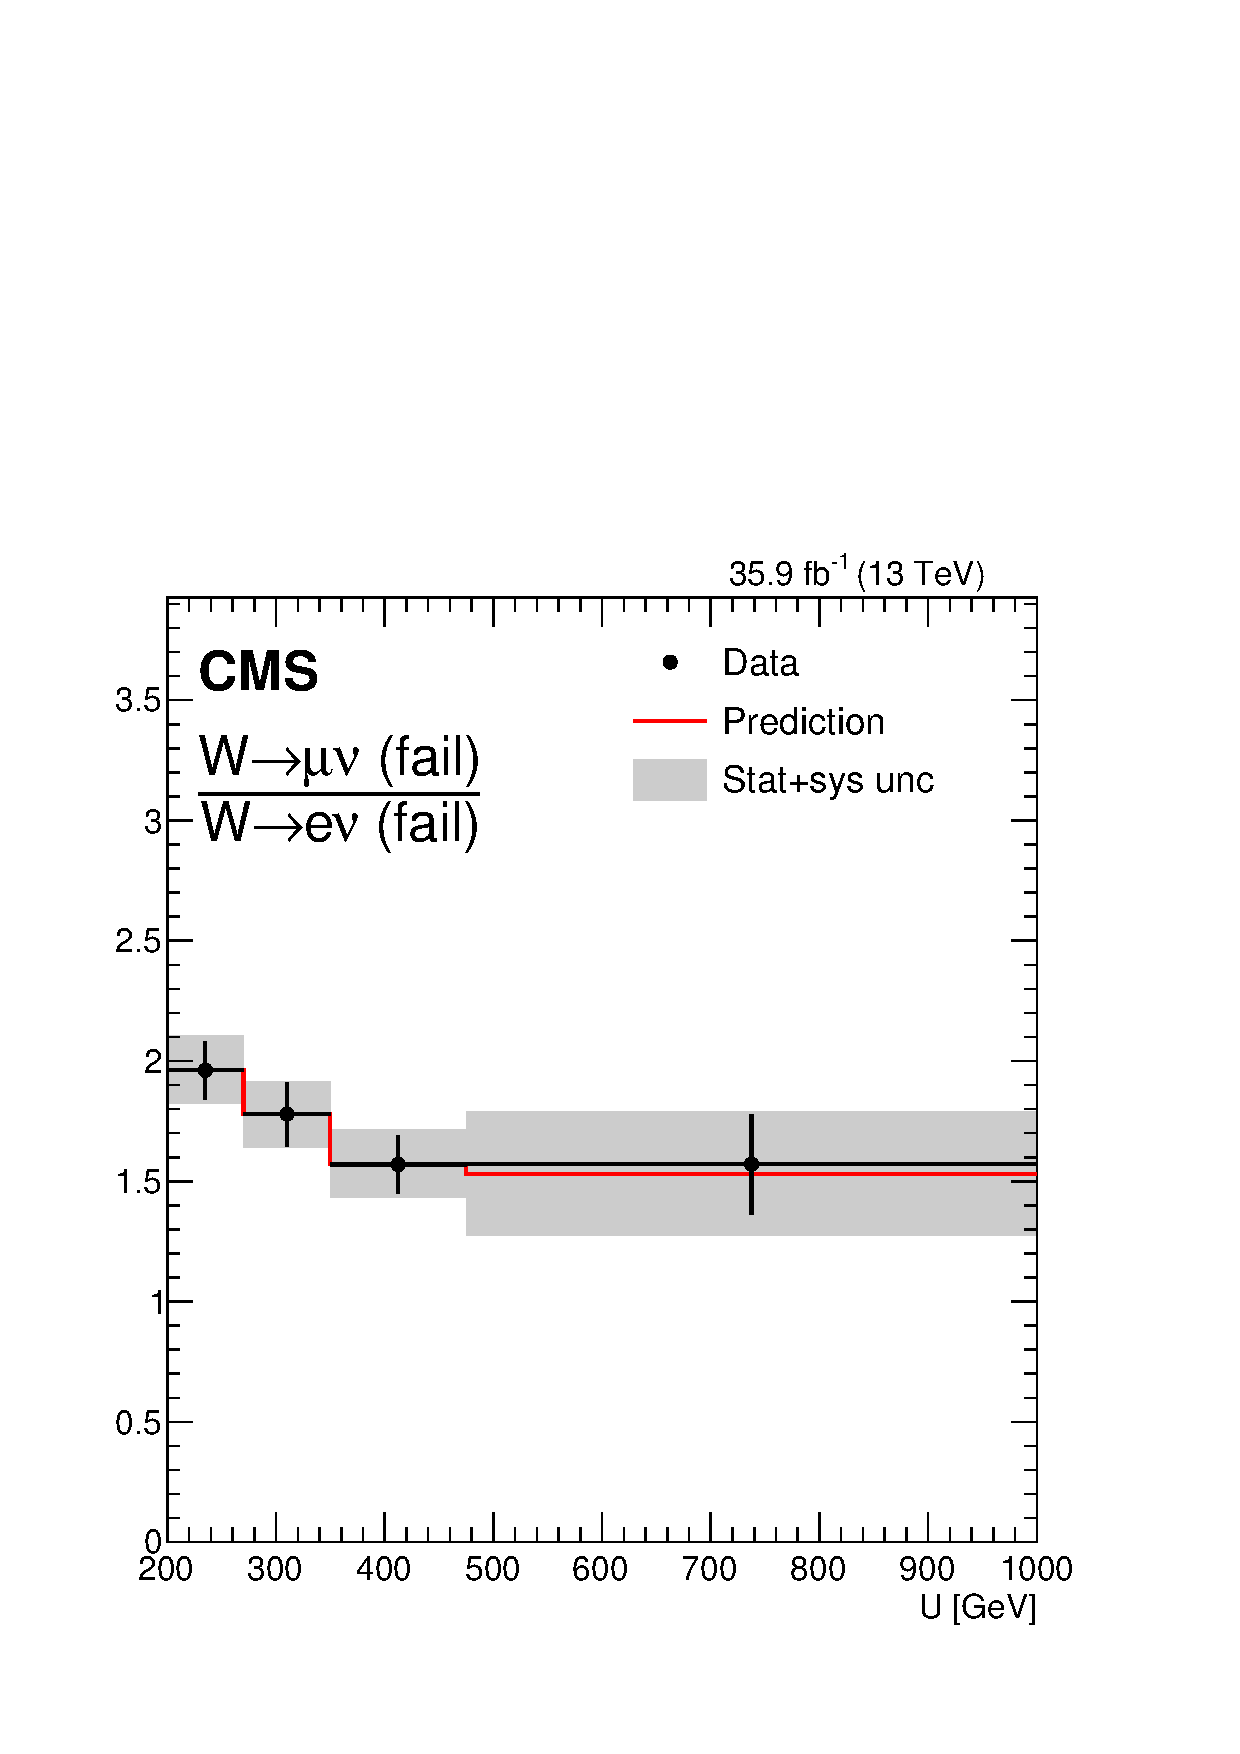
\includegraphics[width=0.45\textwidth]{figures/pullsImpact/ratio_wmn_fail_wen_fail_shapes_fit_b.pdf}\\
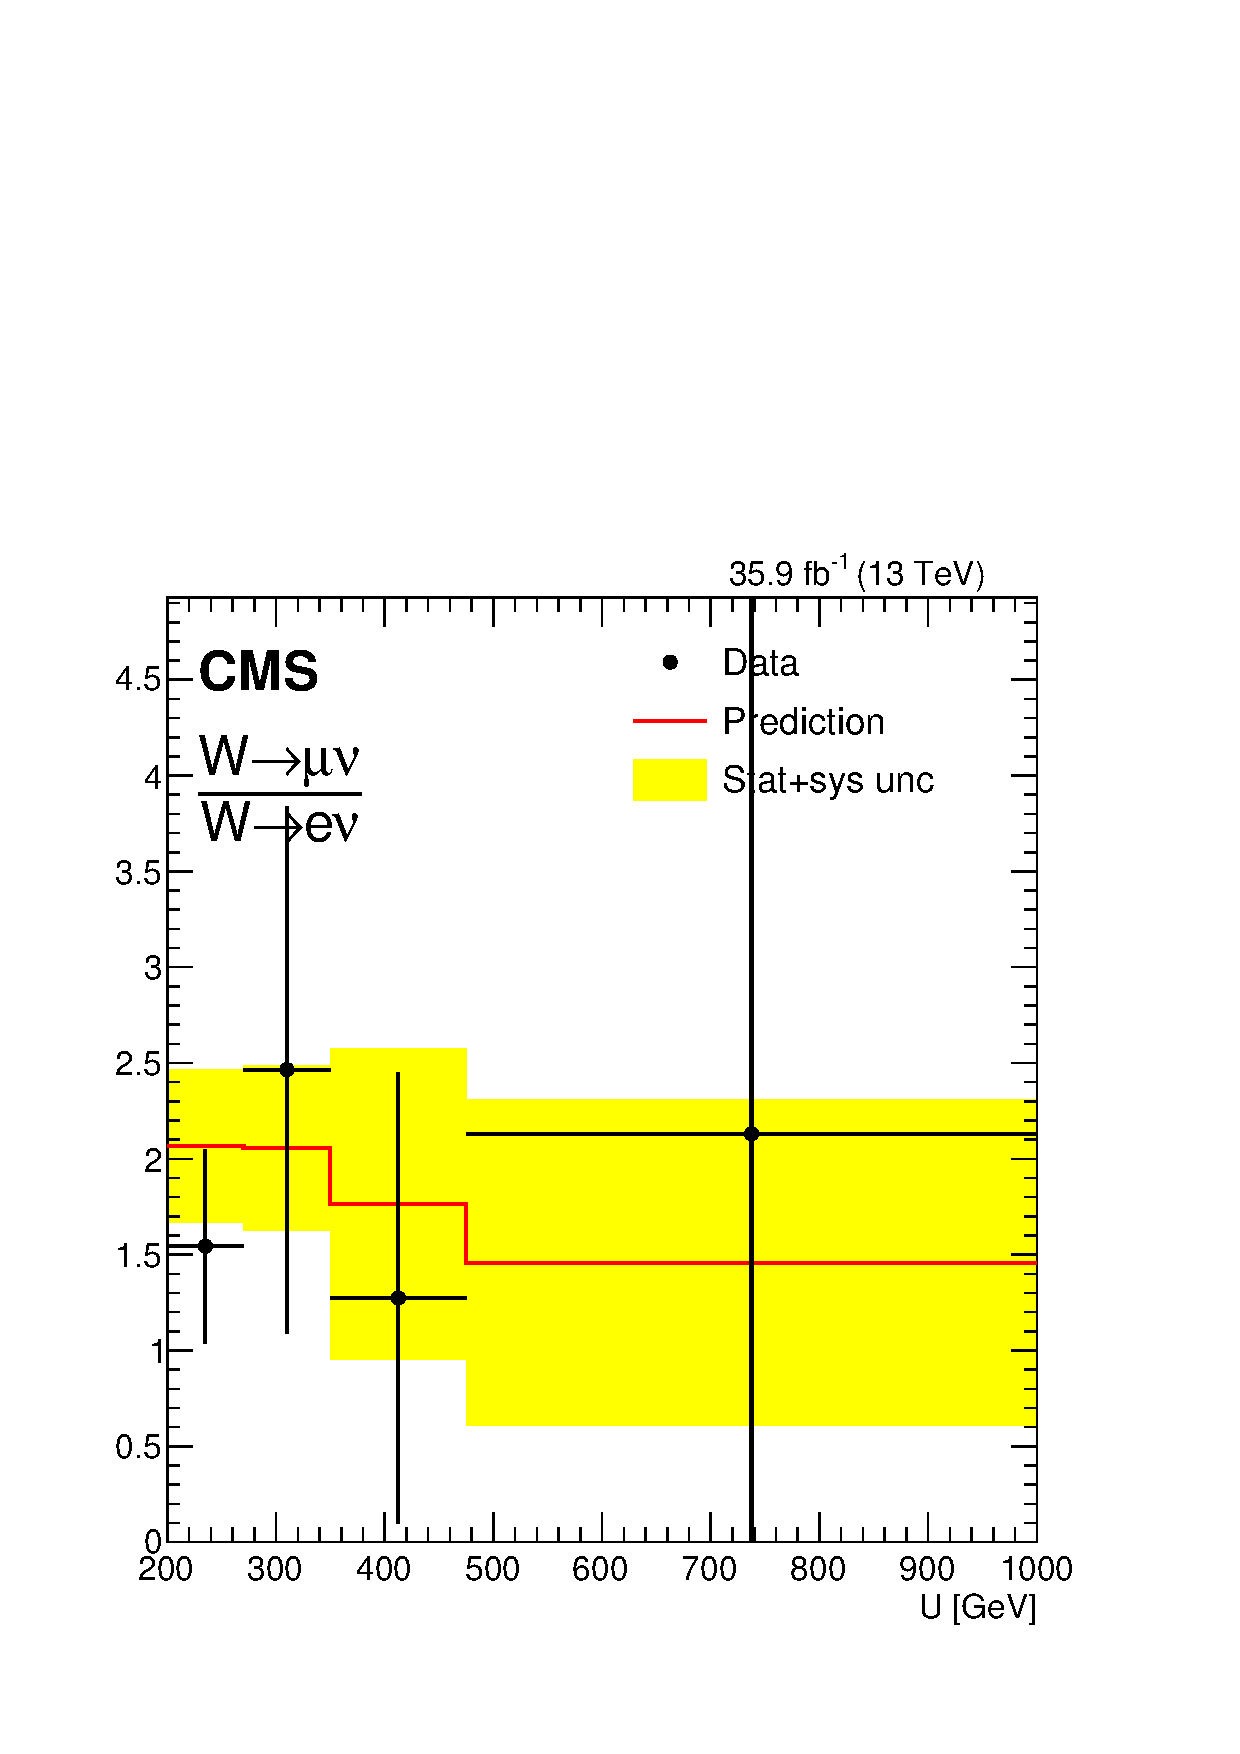
\includegraphics[width=0.45\textwidth]{figures/pullsImpact/ratio_wmn_wen_shapes_prefit.pdf}
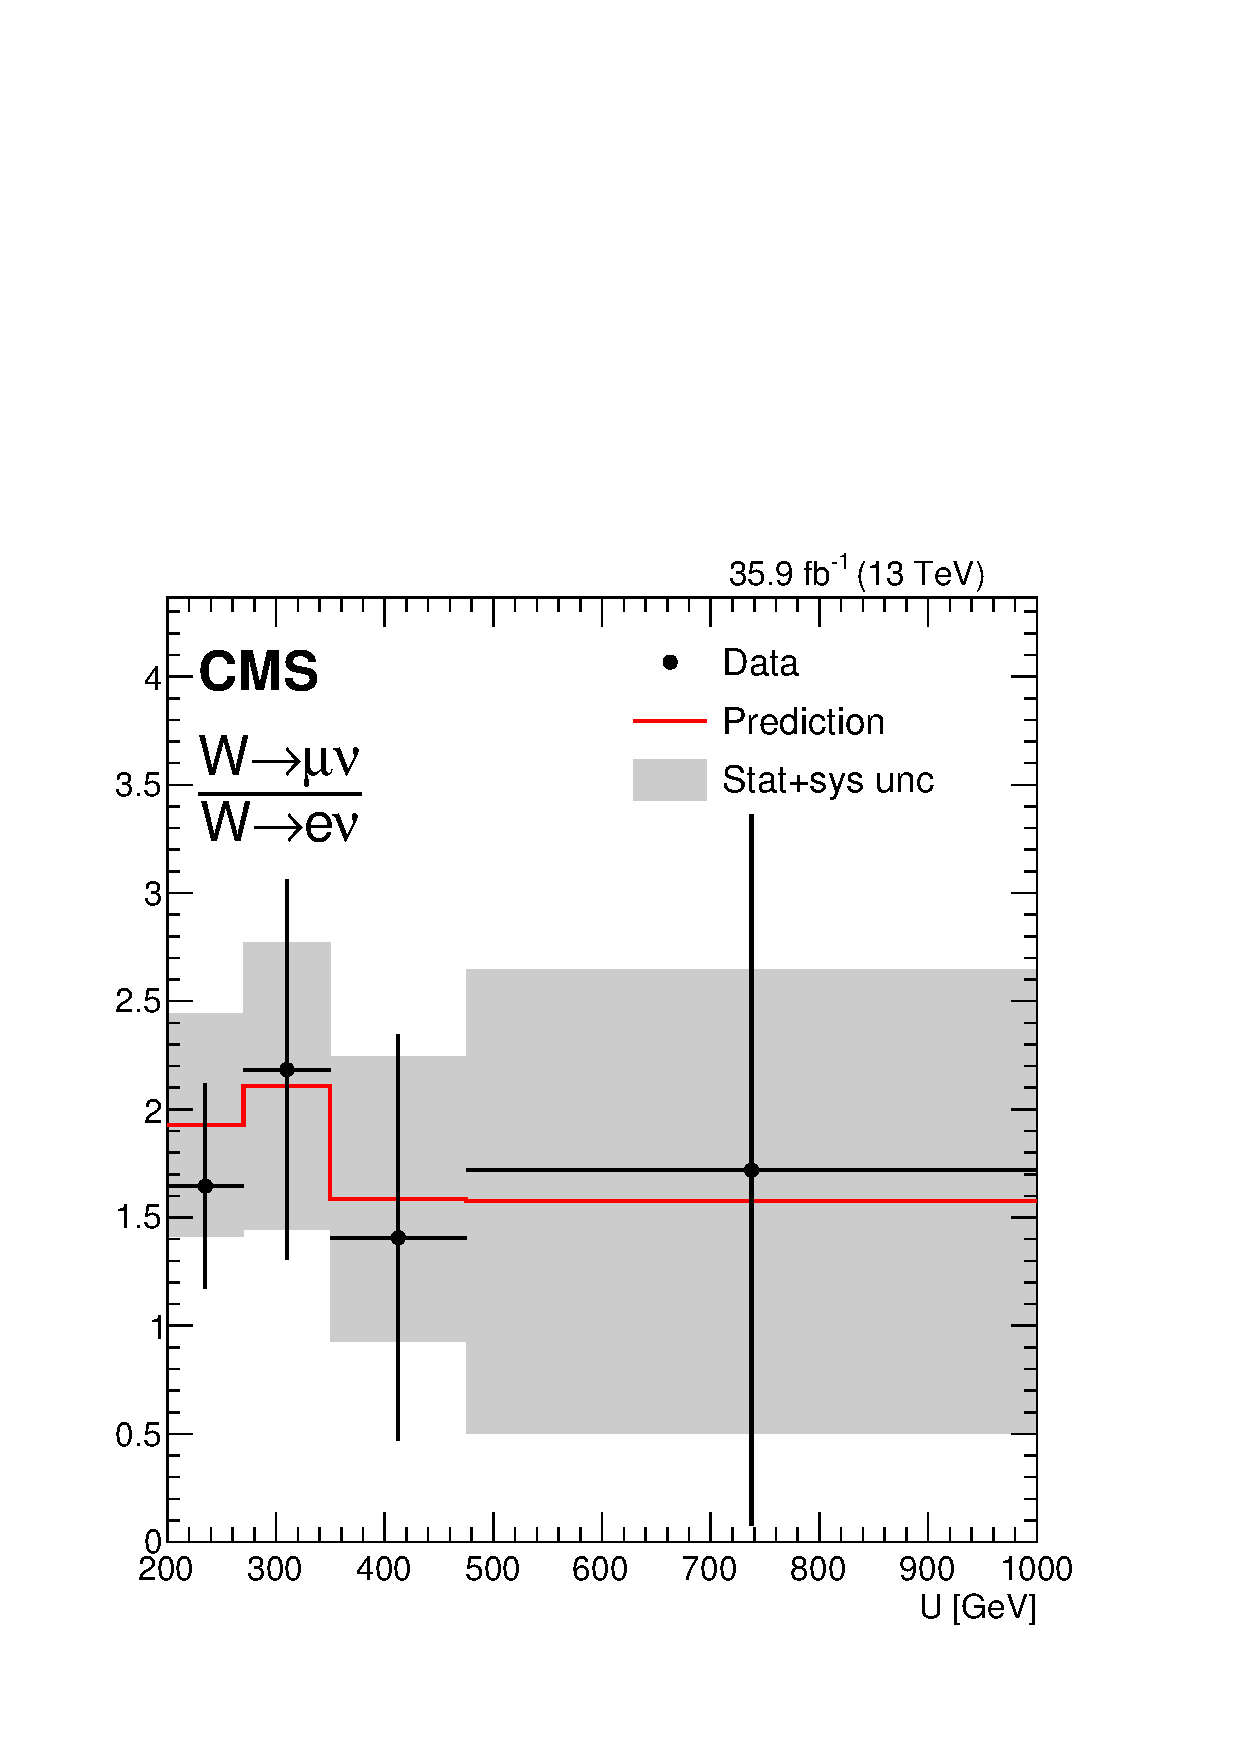
\includegraphics[width=0.45\textwidth]{figures/pullsImpact/ratio_wmn_wen_shapes_fit_b.pdf}\\
\caption{Ratios of pre-fit (left column) and post-fit (right column) templates for W+jets processes in the W pass/fail regions. Black dots indicate the ratio of data yields (after subtracting trailing backgrounds) and demonstrate good agreement between data and simulation.}
\label{wwratios}
\end{figure}

\clearpage

\begin{figure}
\centering
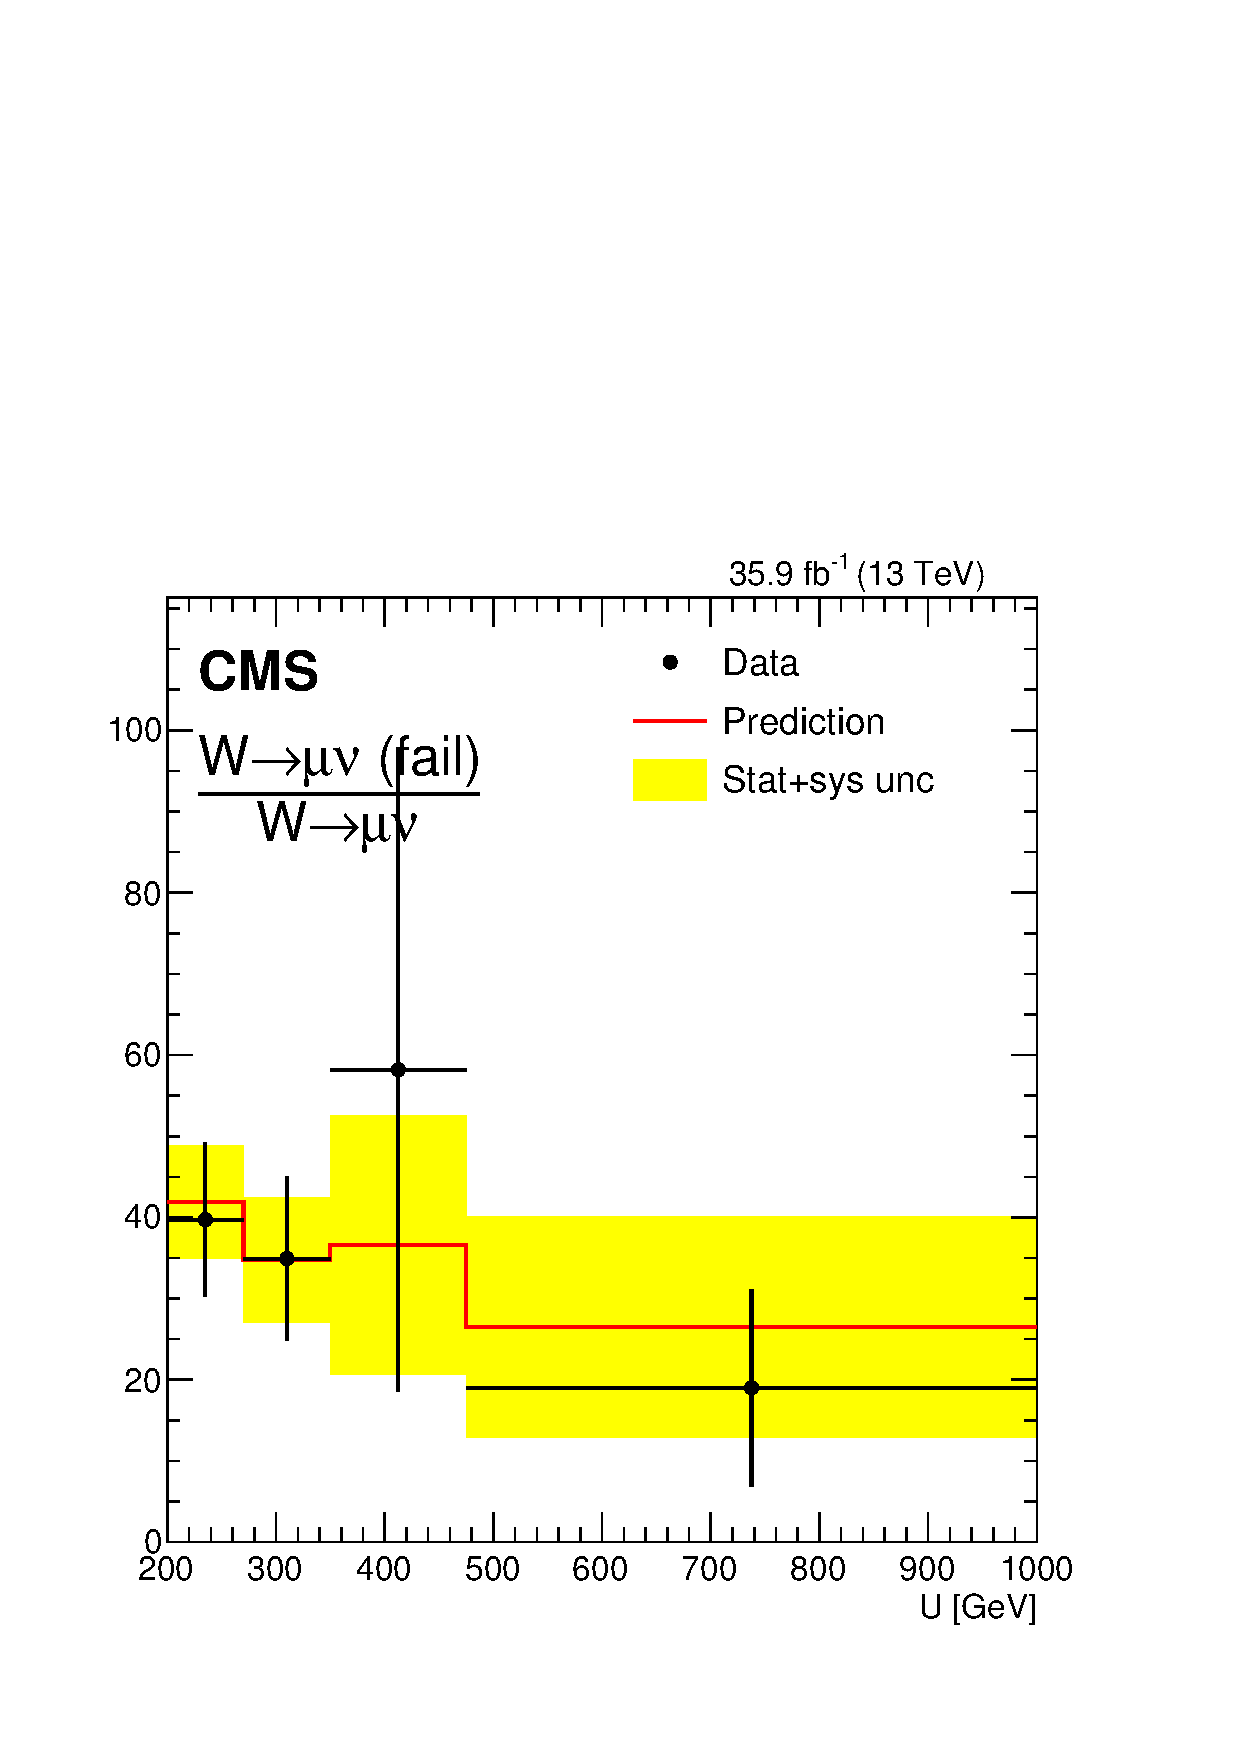
\includegraphics[width=0.45\textwidth]{figures/pullsImpact/ratio_wmn_fail_wmn_shapes_prefit.pdf}
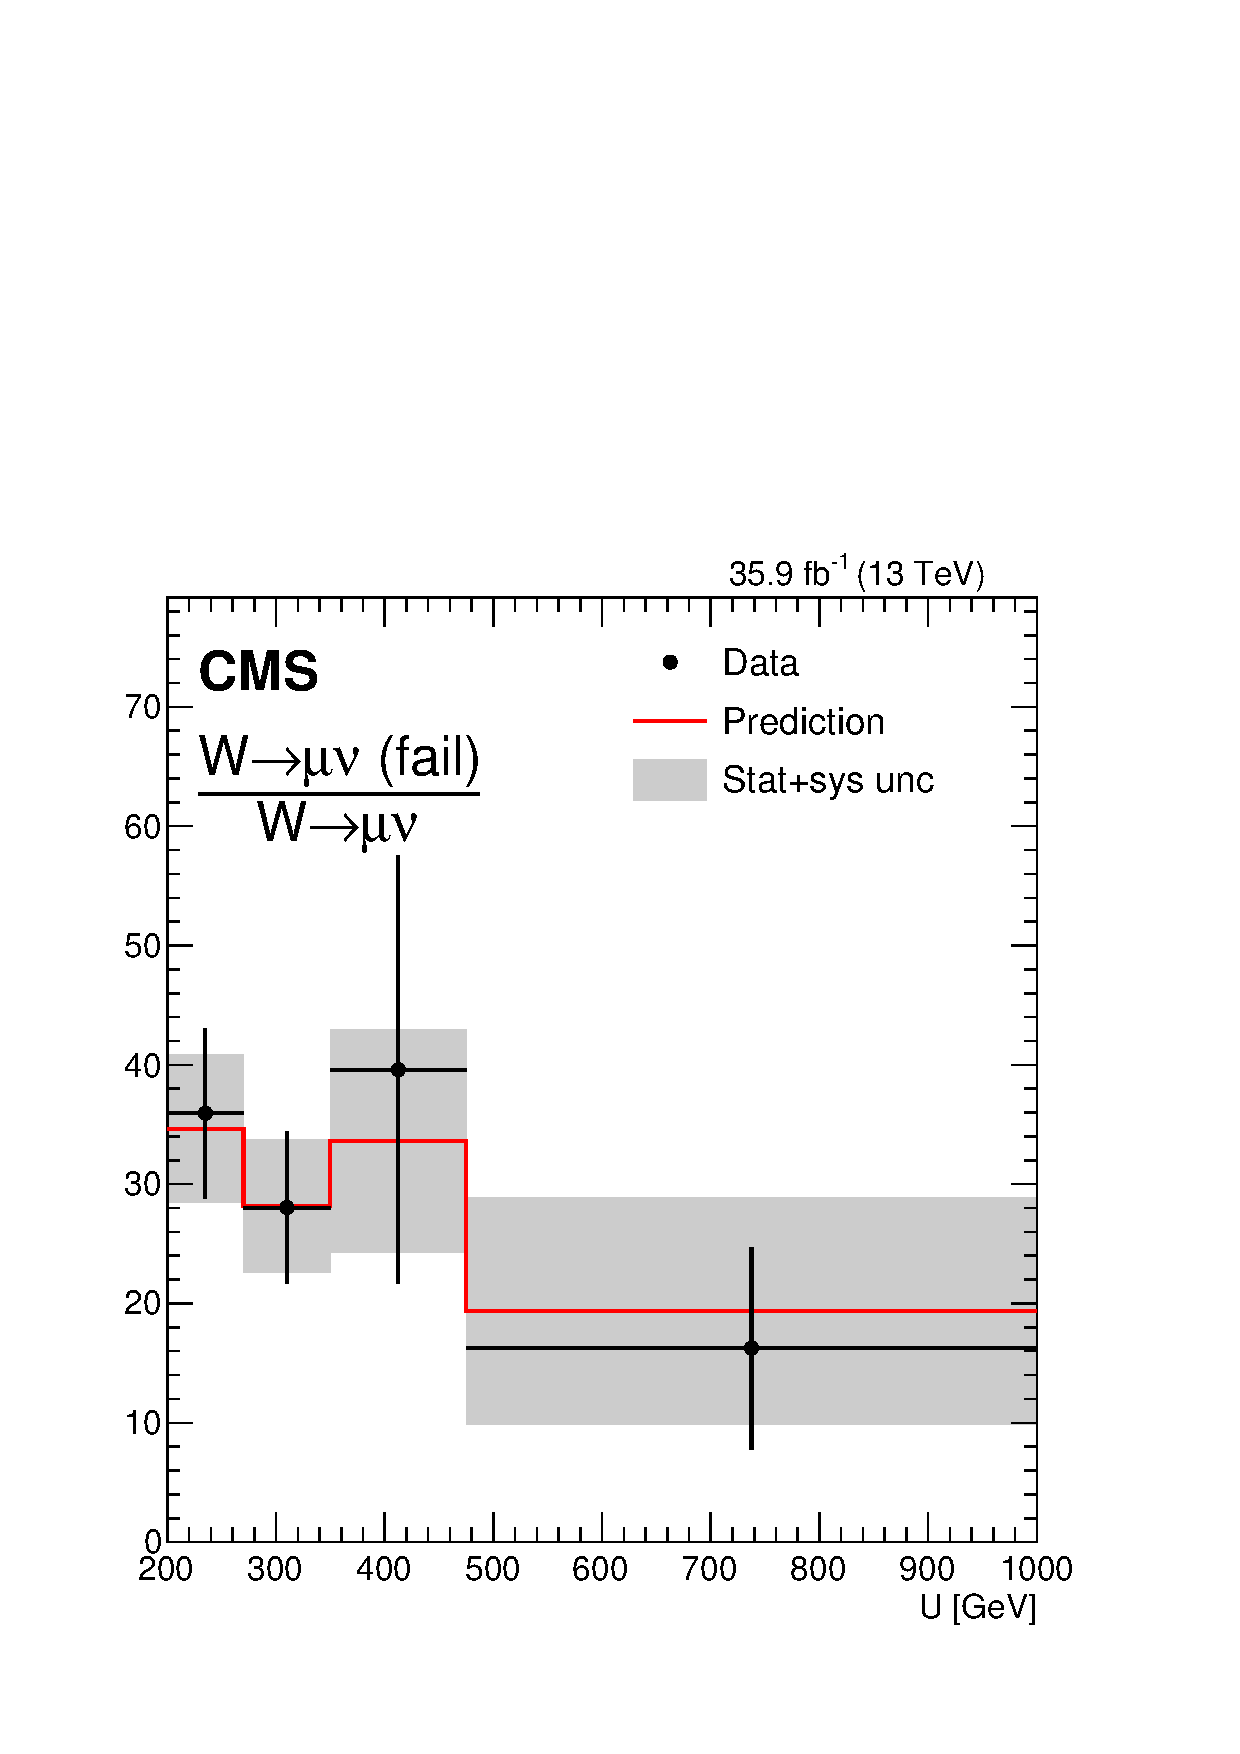
\includegraphics[width=0.45\textwidth]{figures/pullsImpact/ratio_wmn_fail_wmn_shapes_fit_b.pdf}\\
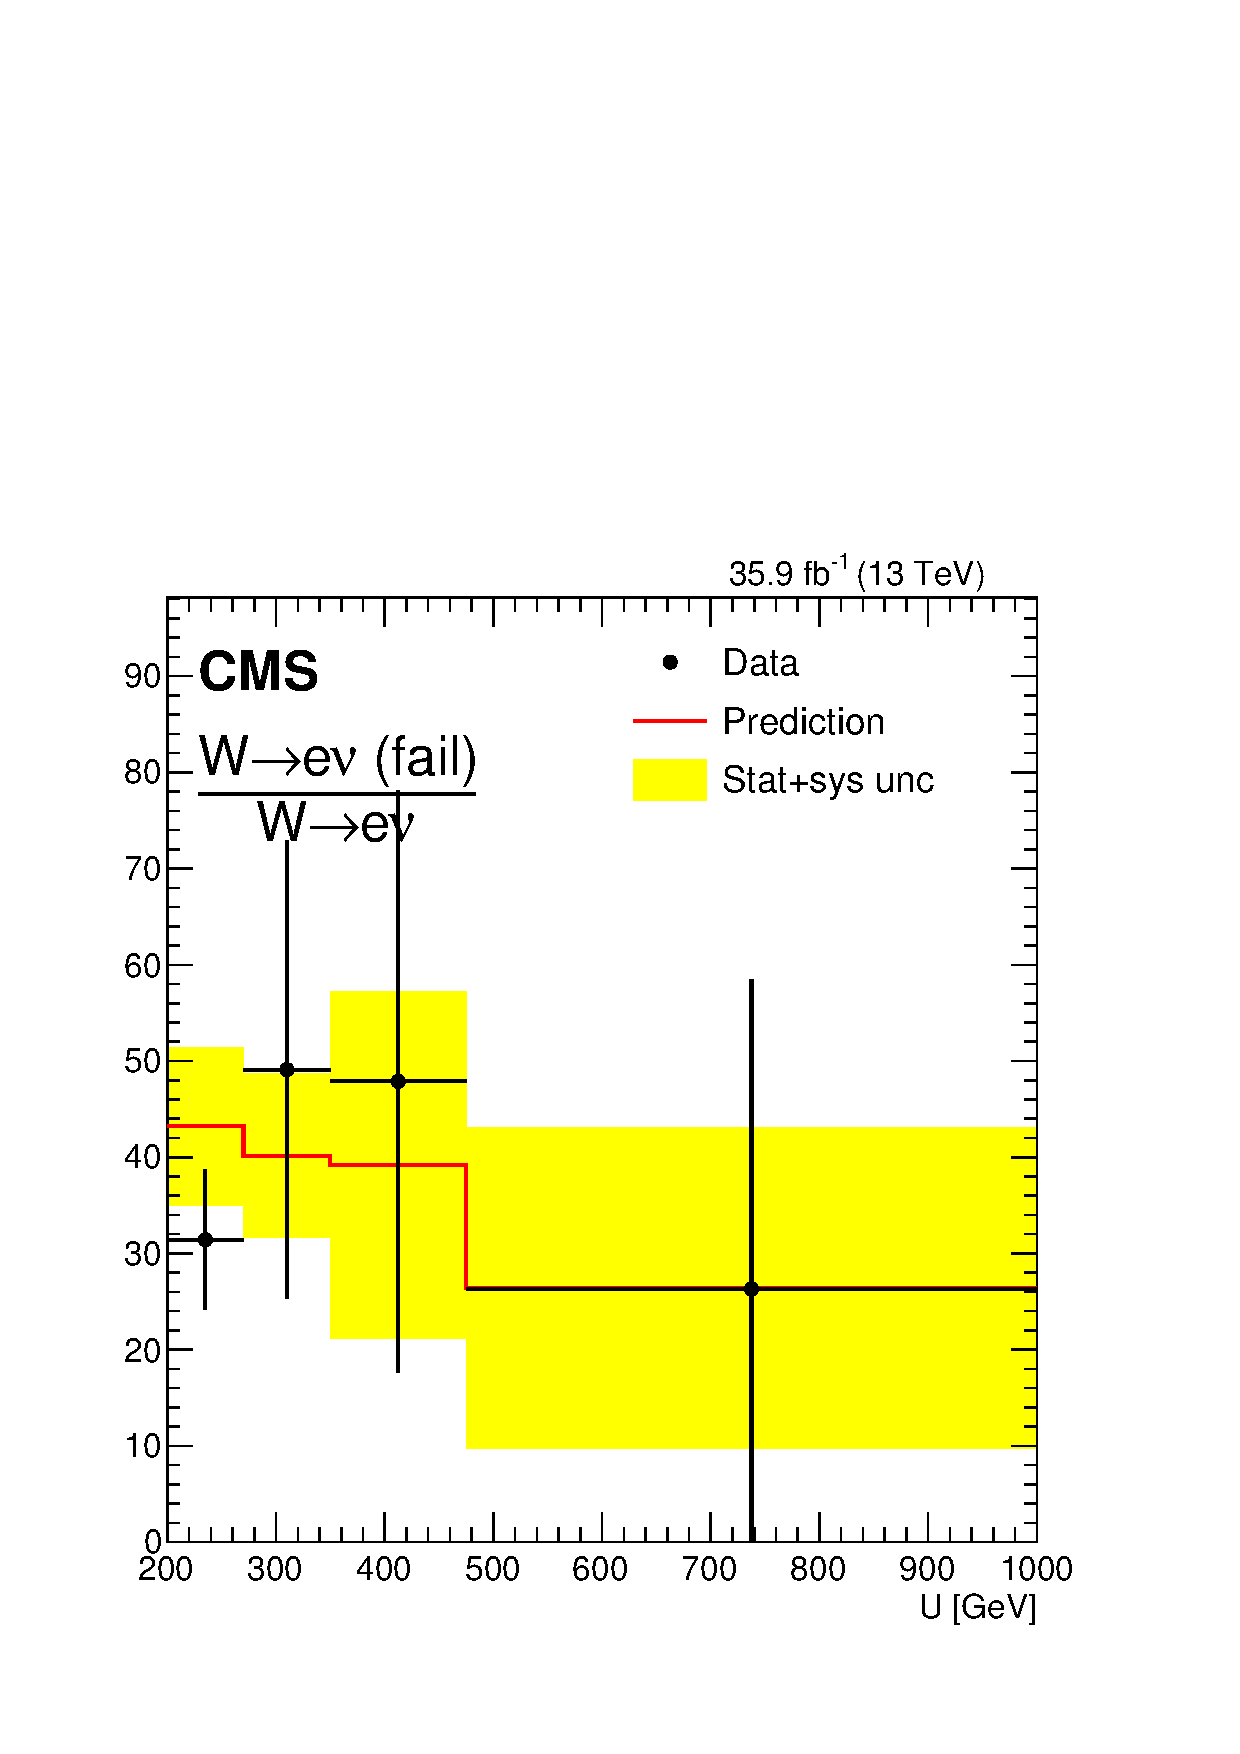
\includegraphics[width=0.45\textwidth]{figures/pullsImpact/ratio_wen_fail_wen_shapes_prefit.pdf}
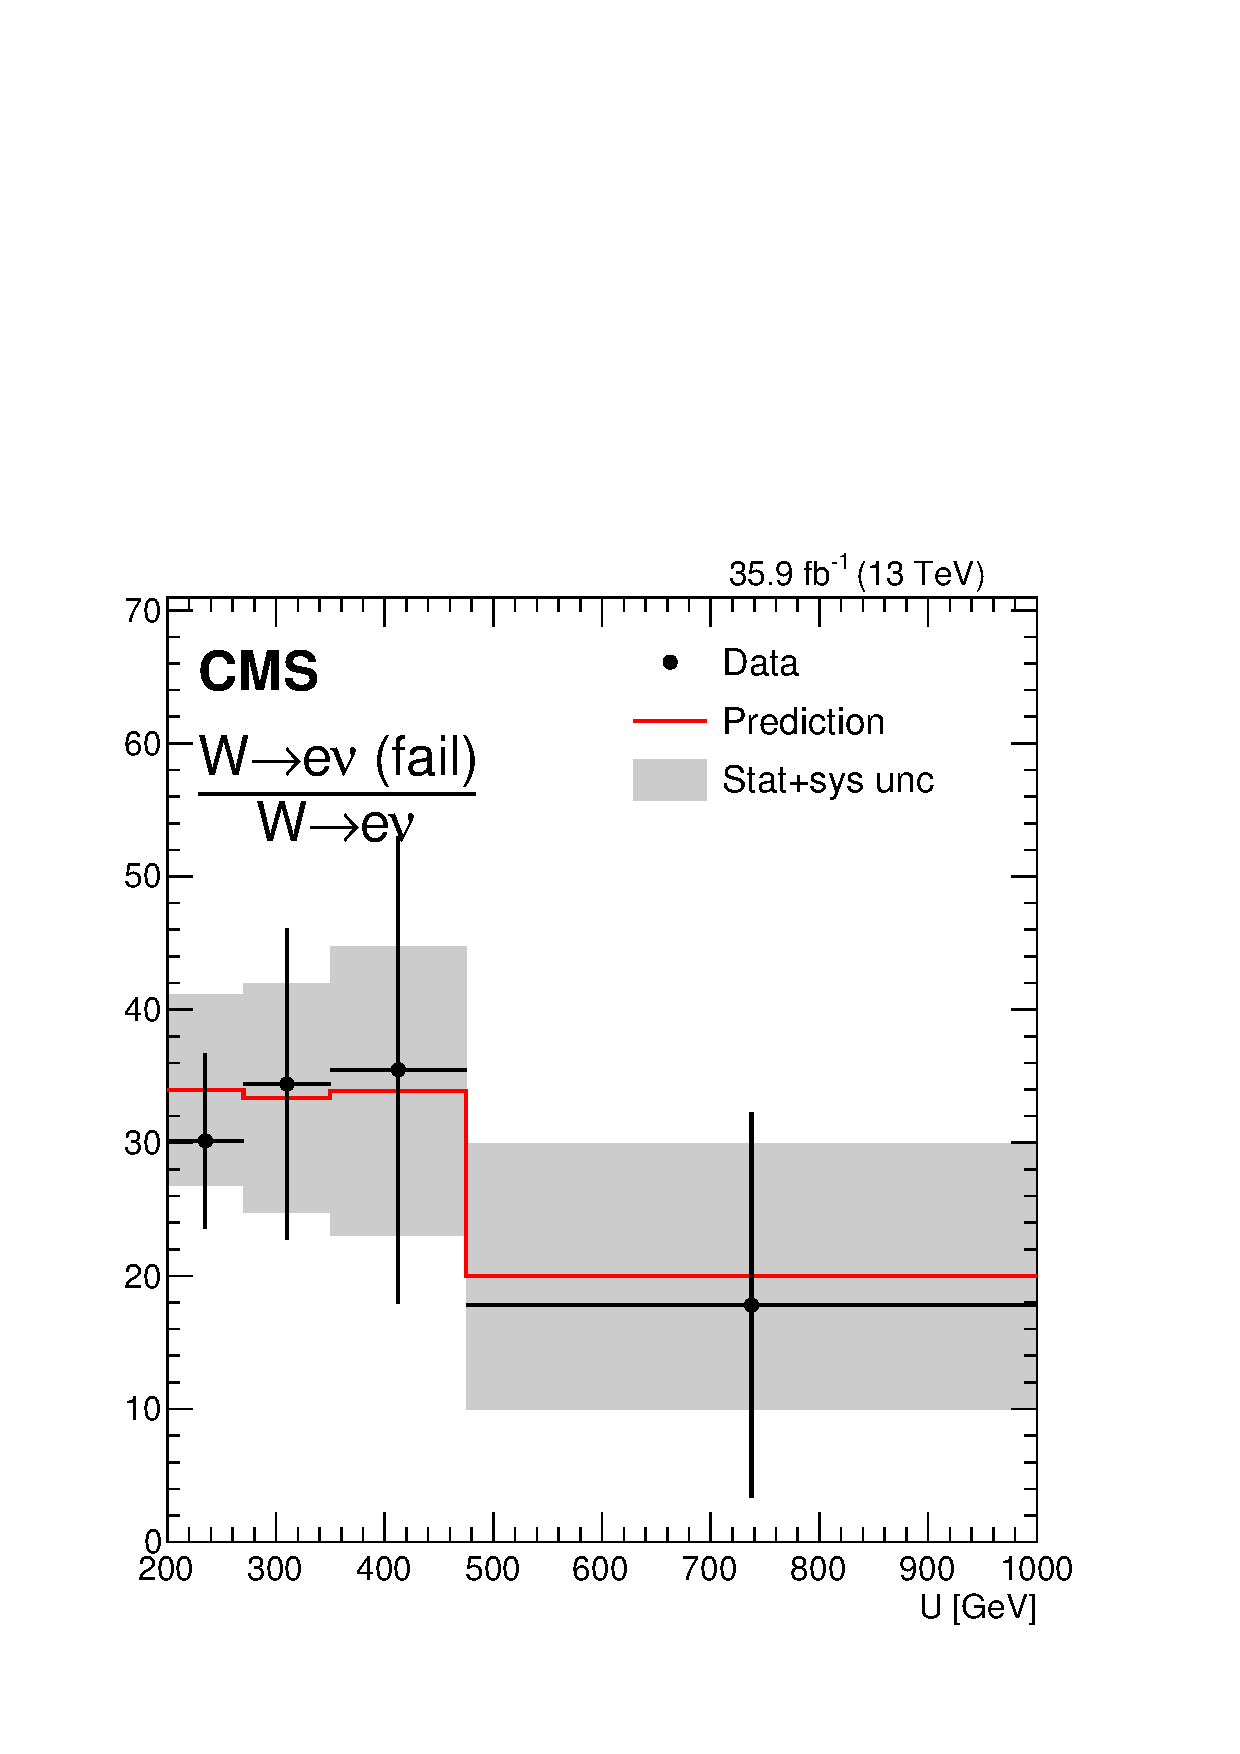
\includegraphics[width=0.45\textwidth]{figures/pullsImpact/ratio_wen_fail_wen_shapes_fit_b.pdf}\\
\caption{Ratios of pre-fit (left column) and post-fit (right column) templates for W+jets processes in the W pass/fail regions. Black dots indicate the ratio of data yields (after subtracting trailing backgrounds) and demonstrate good agreement between data and simulation.}
\label{wwratios}
\end{figure}

\clearpage

\begin{figure}
\centering
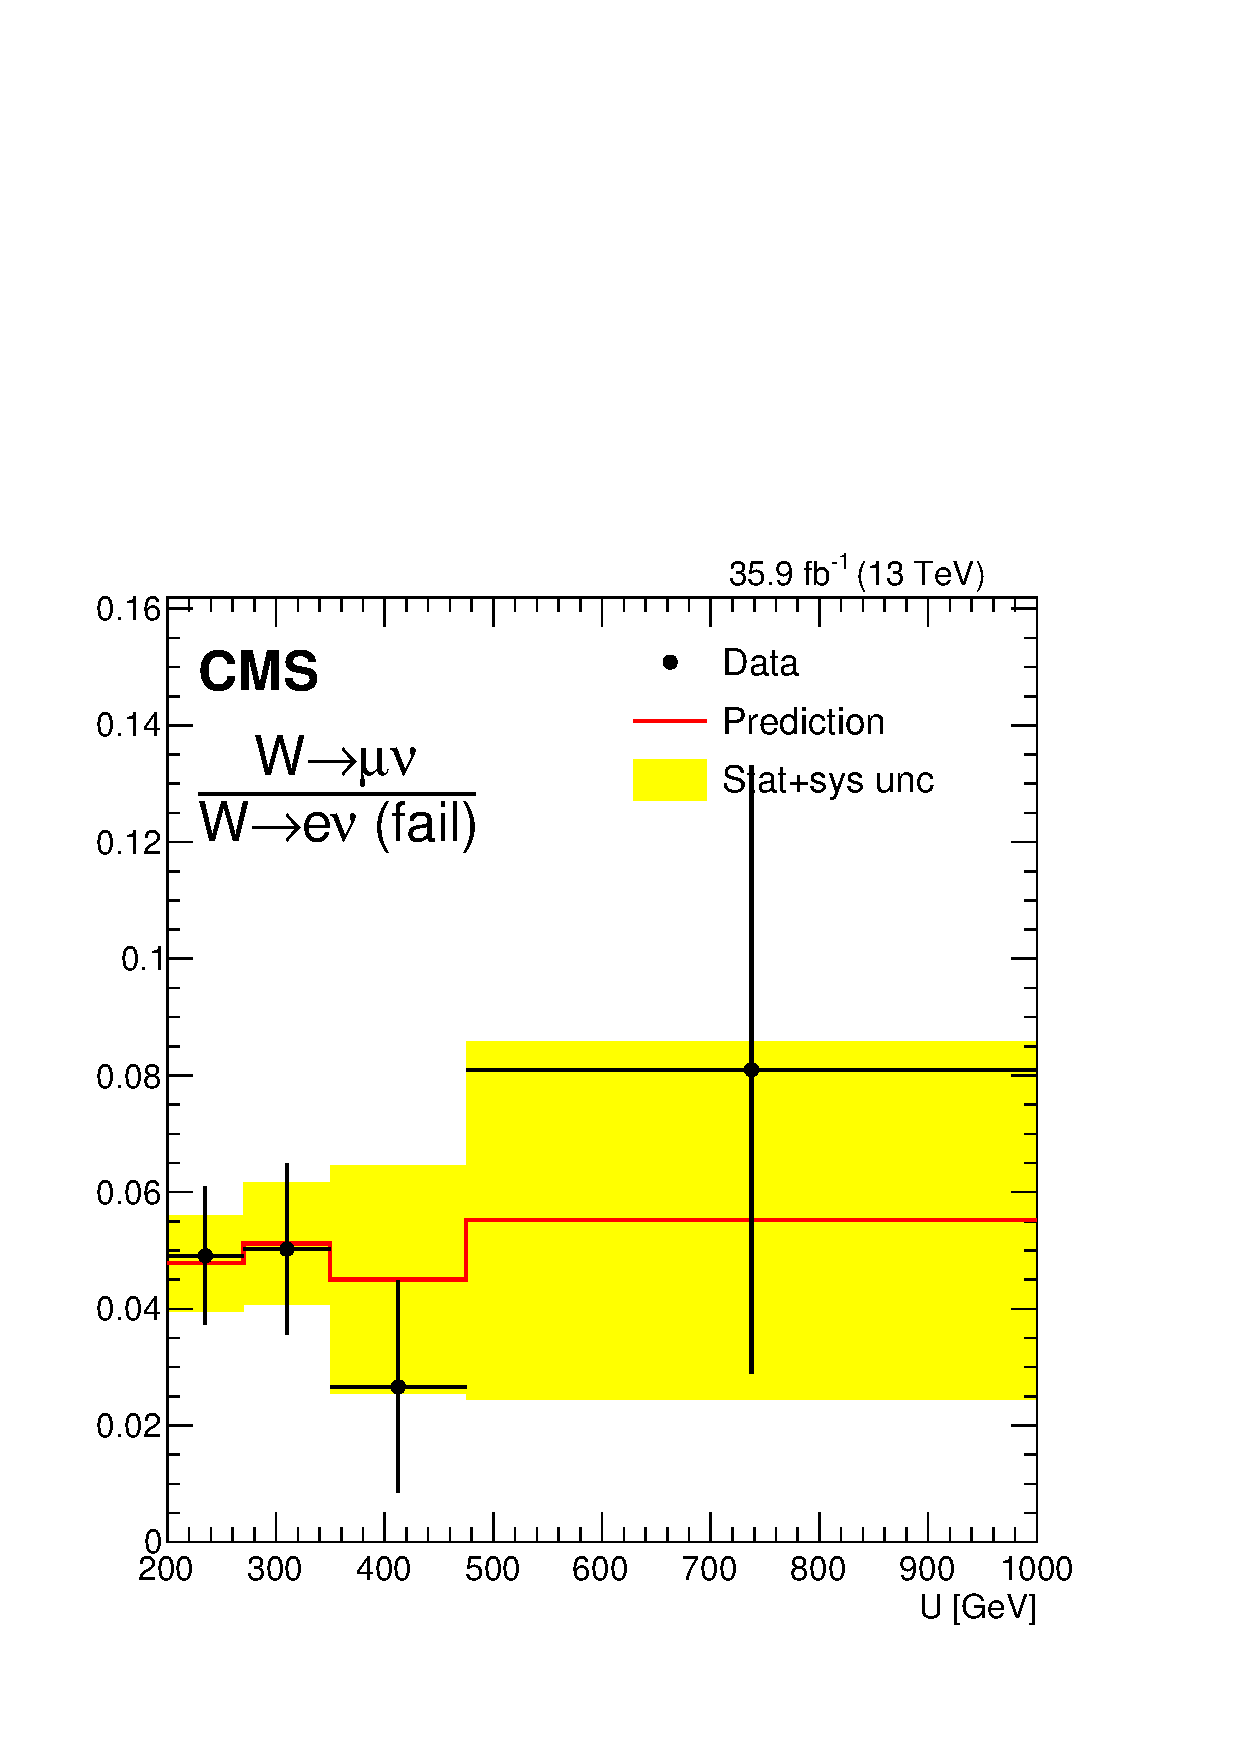
\includegraphics[width=0.45\textwidth]{figures/pullsImpact/ratio_wmn_wen_fail_shapes_prefit.pdf}
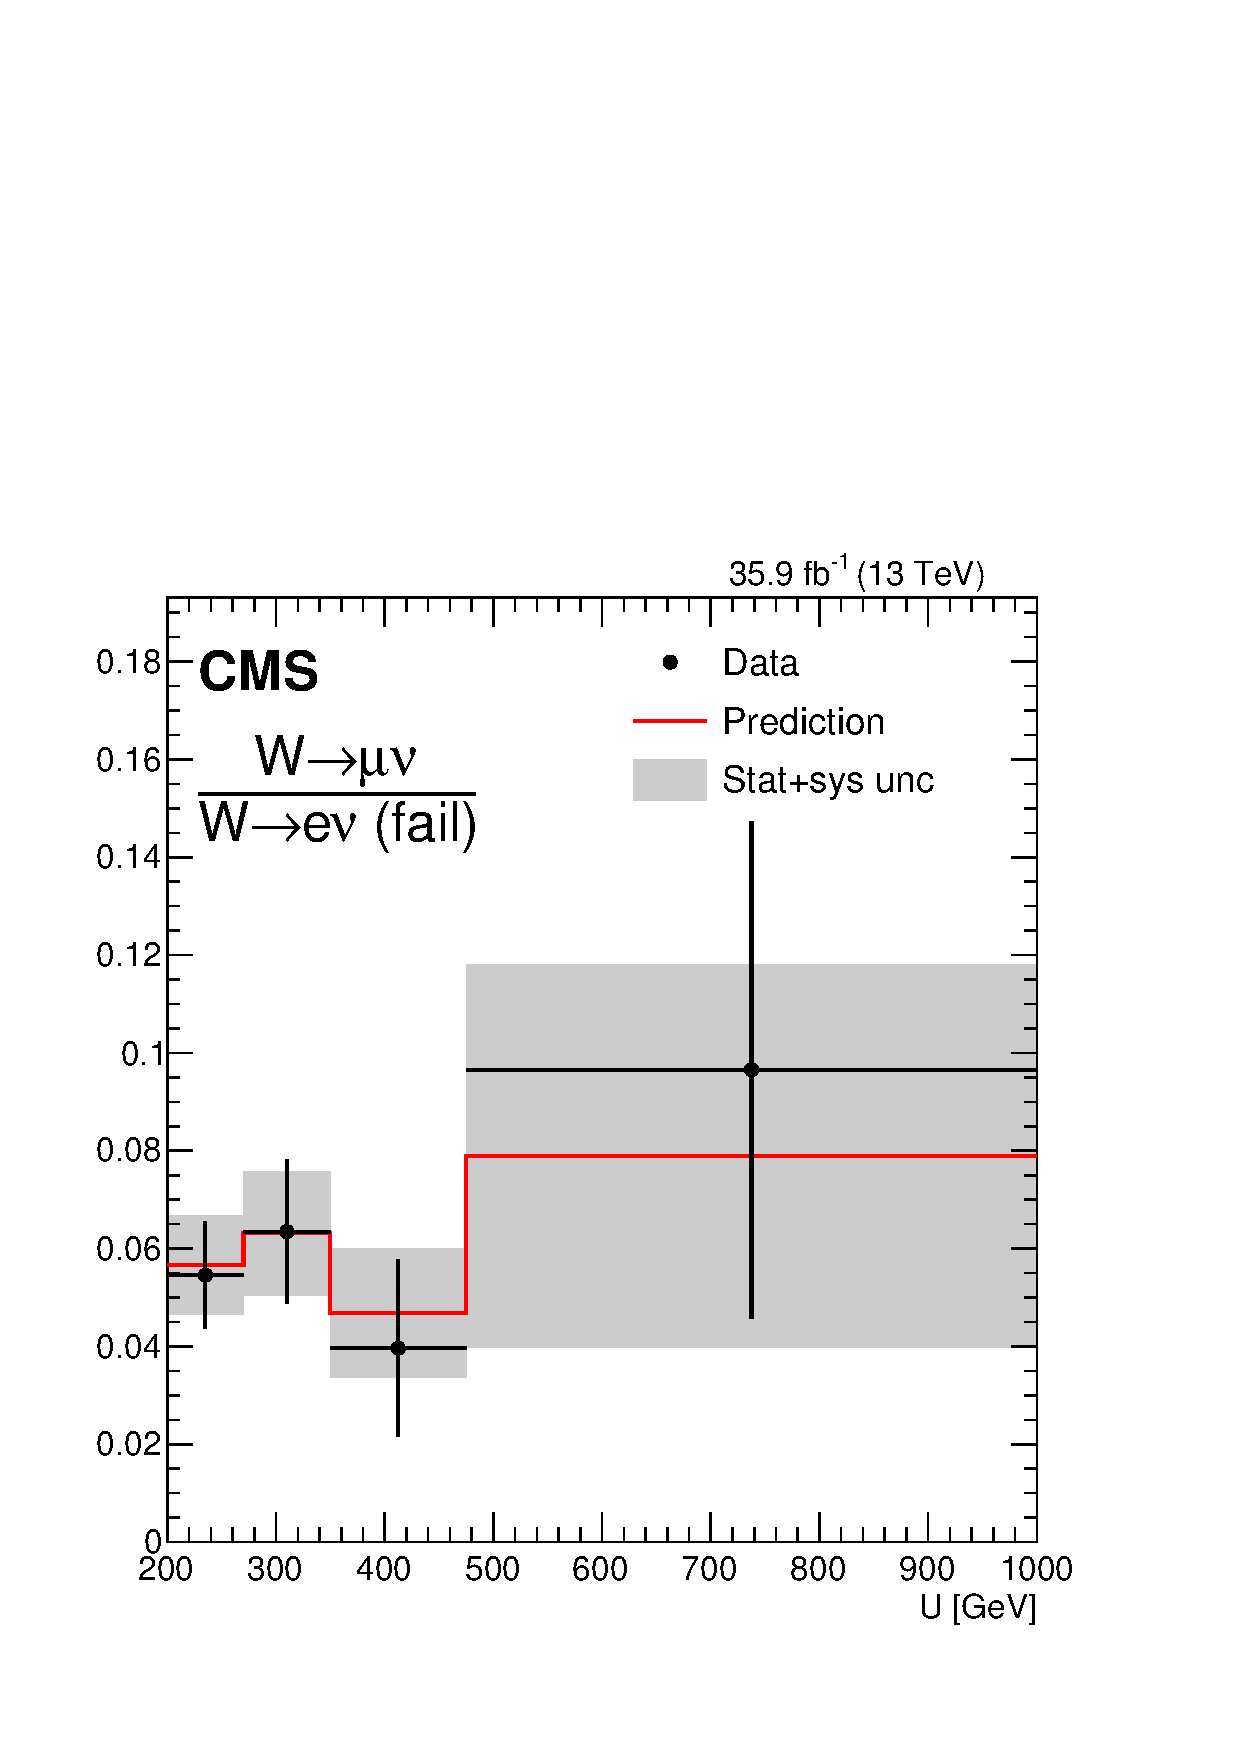
\includegraphics[width=0.45\textwidth]{figures/pullsImpact/ratio_wmn_wen_fail_shapes_fit_b.pdf}\\
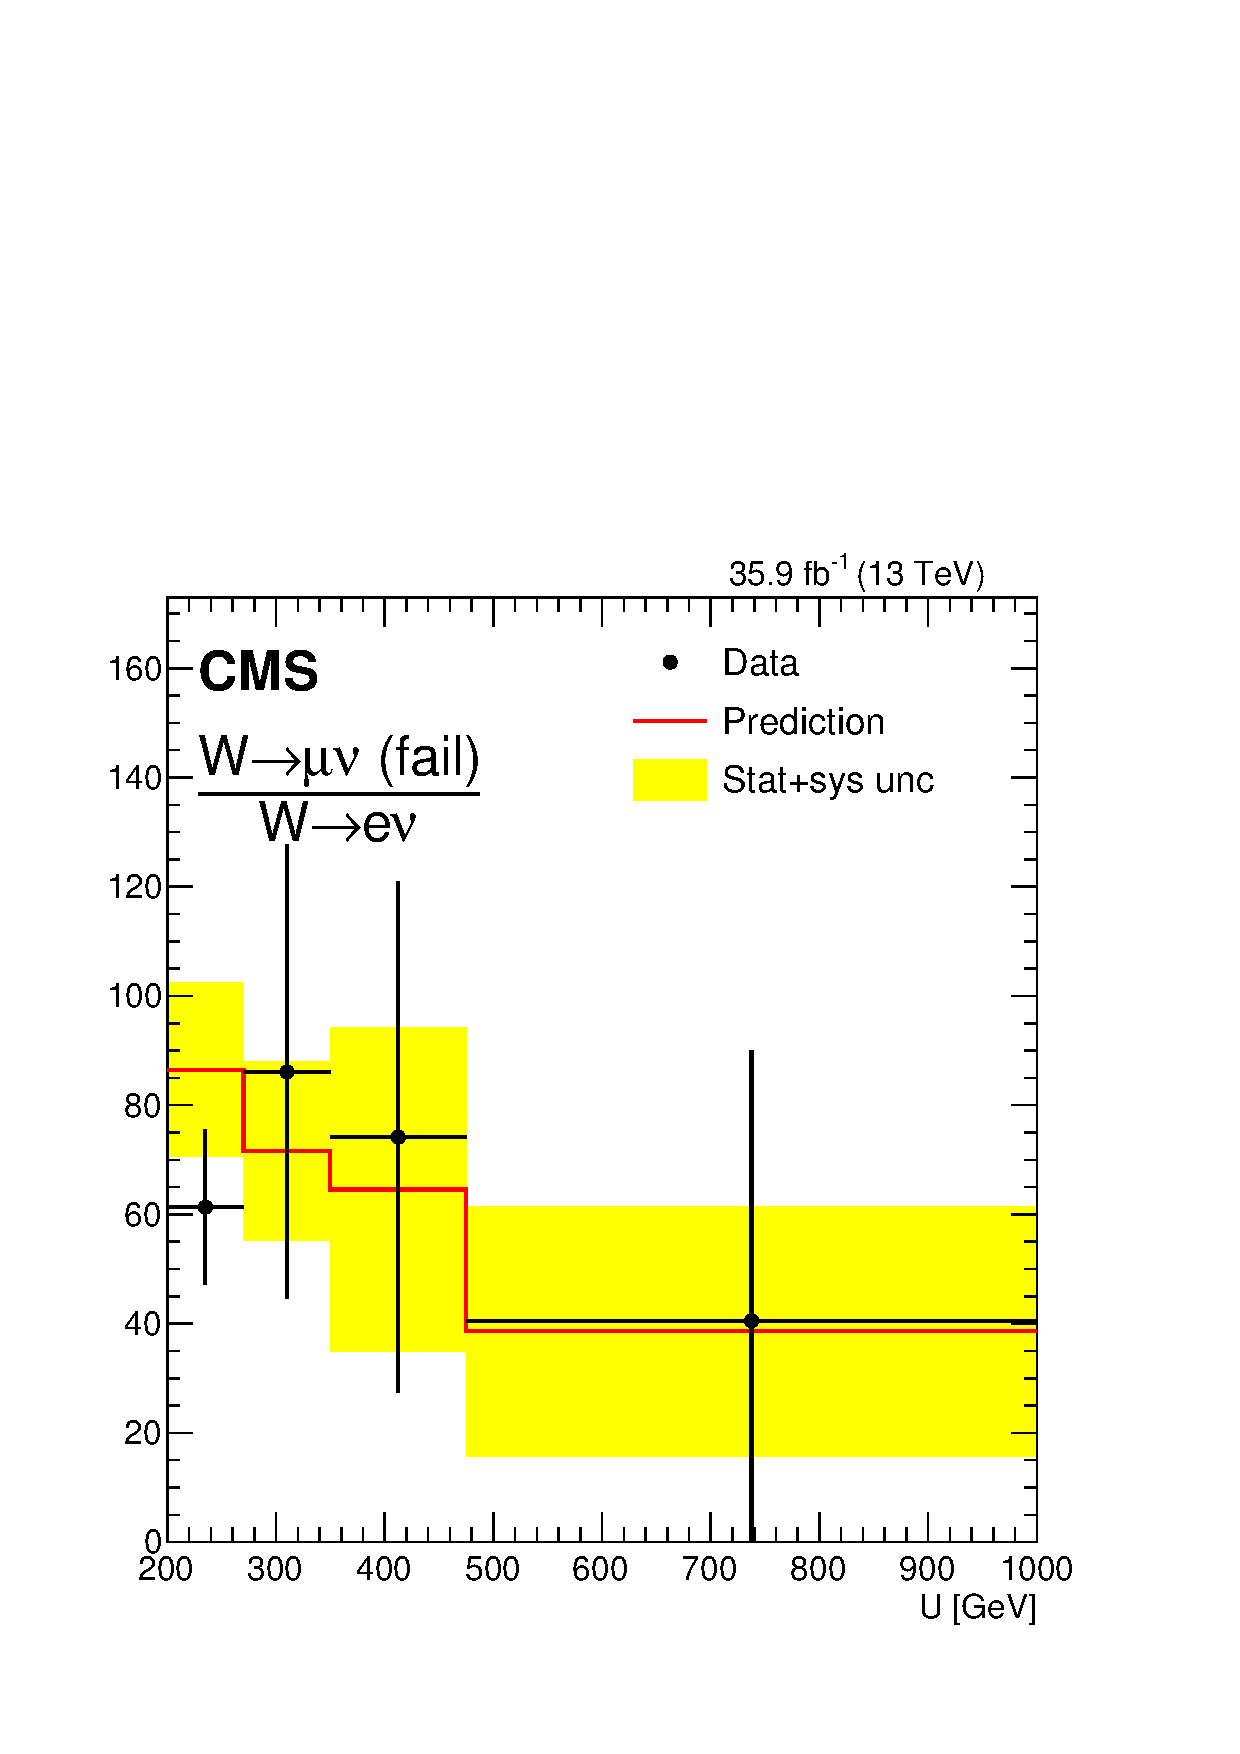
\includegraphics[width=0.45\textwidth]{figures/pullsImpact/ratio_wmn_fail_wen_shapes_prefit.pdf}
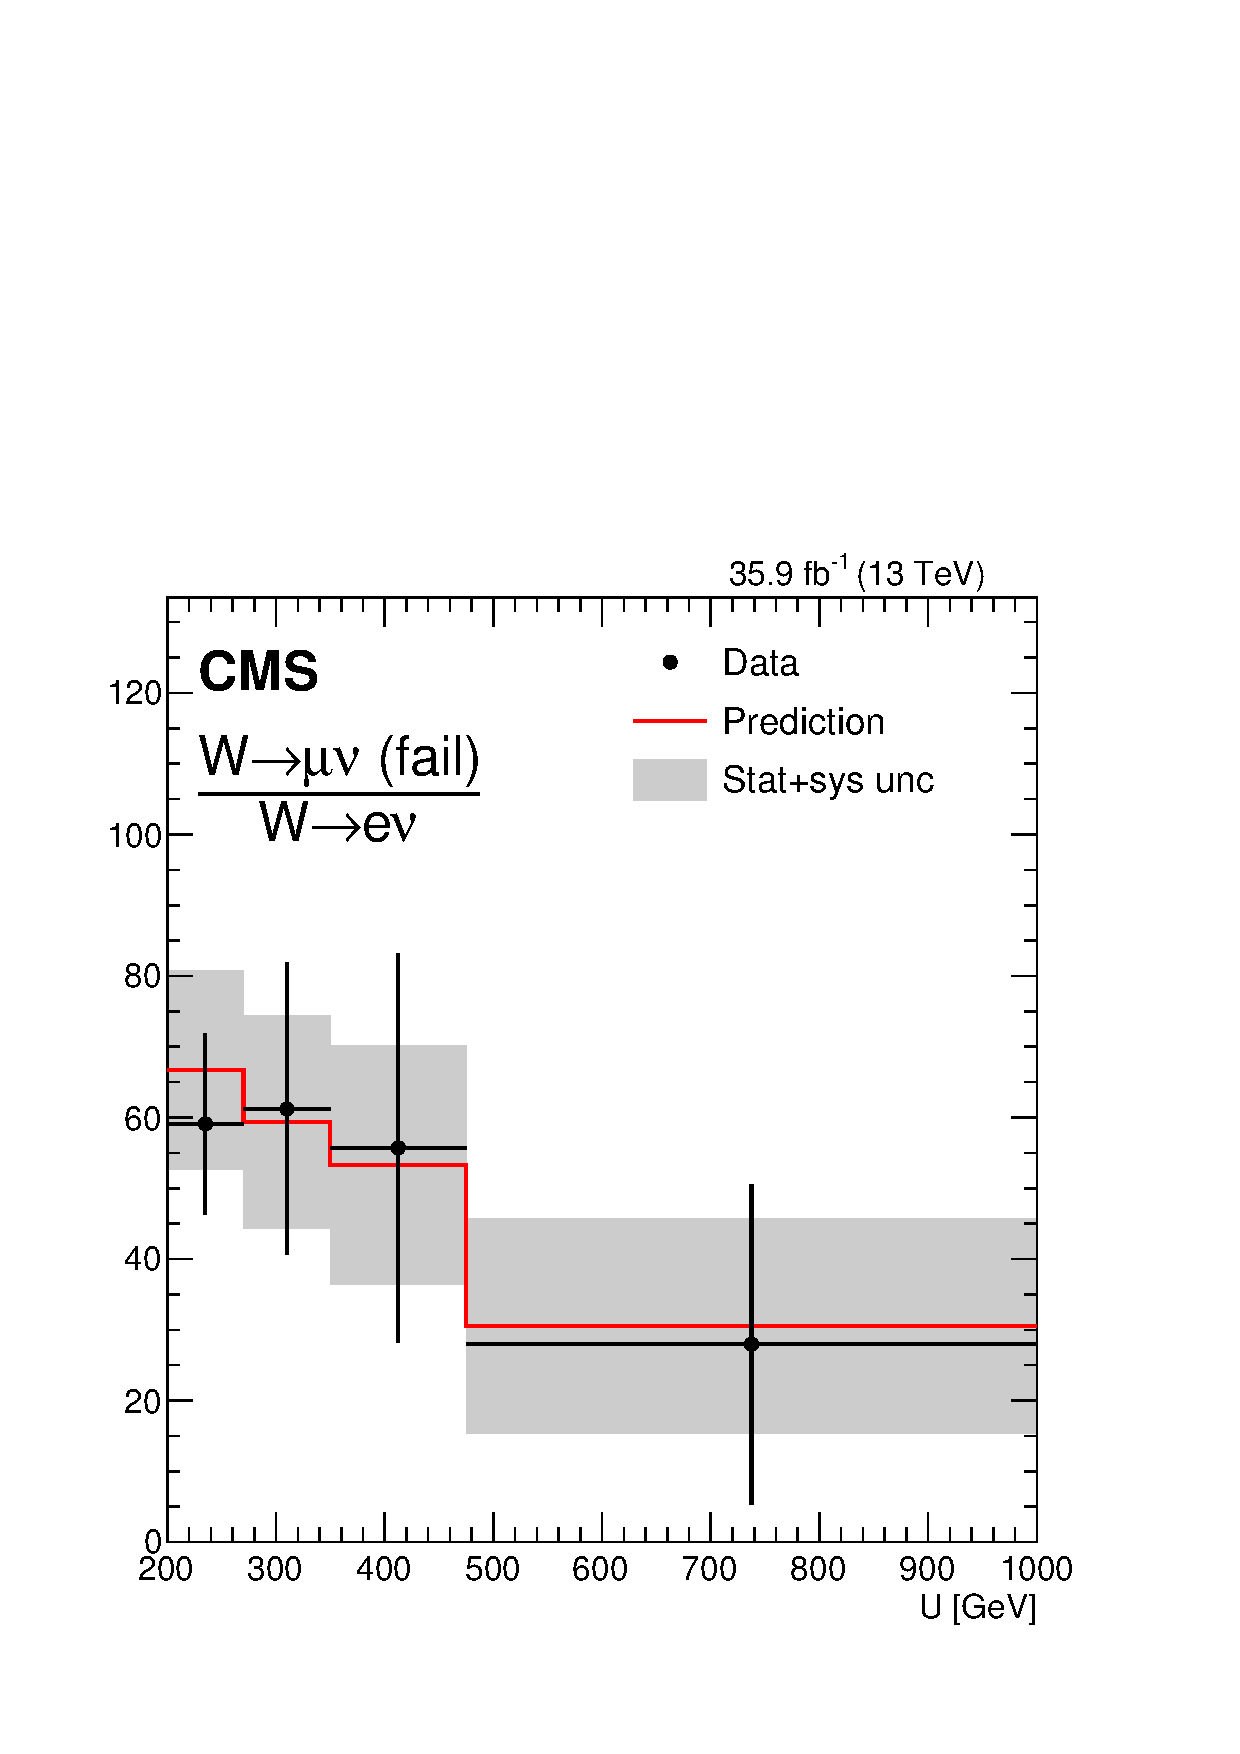
\includegraphics[width=0.45\textwidth]{figures/pullsImpact/ratio_wmn_fail_wen_shapes_fit_b.pdf}\\
\caption{Ratios of pre-fit (left column) and post-fit (right column) templates for W+jets processes in the W pass/fail regions. Black dots indicate the ratio of data yields (after subtracting trailing backgrounds) and demonstrate good agreement between data and simulation.}
\label{wwratios}
\end{figure}

\clearpage

\begin{figure}
\centering
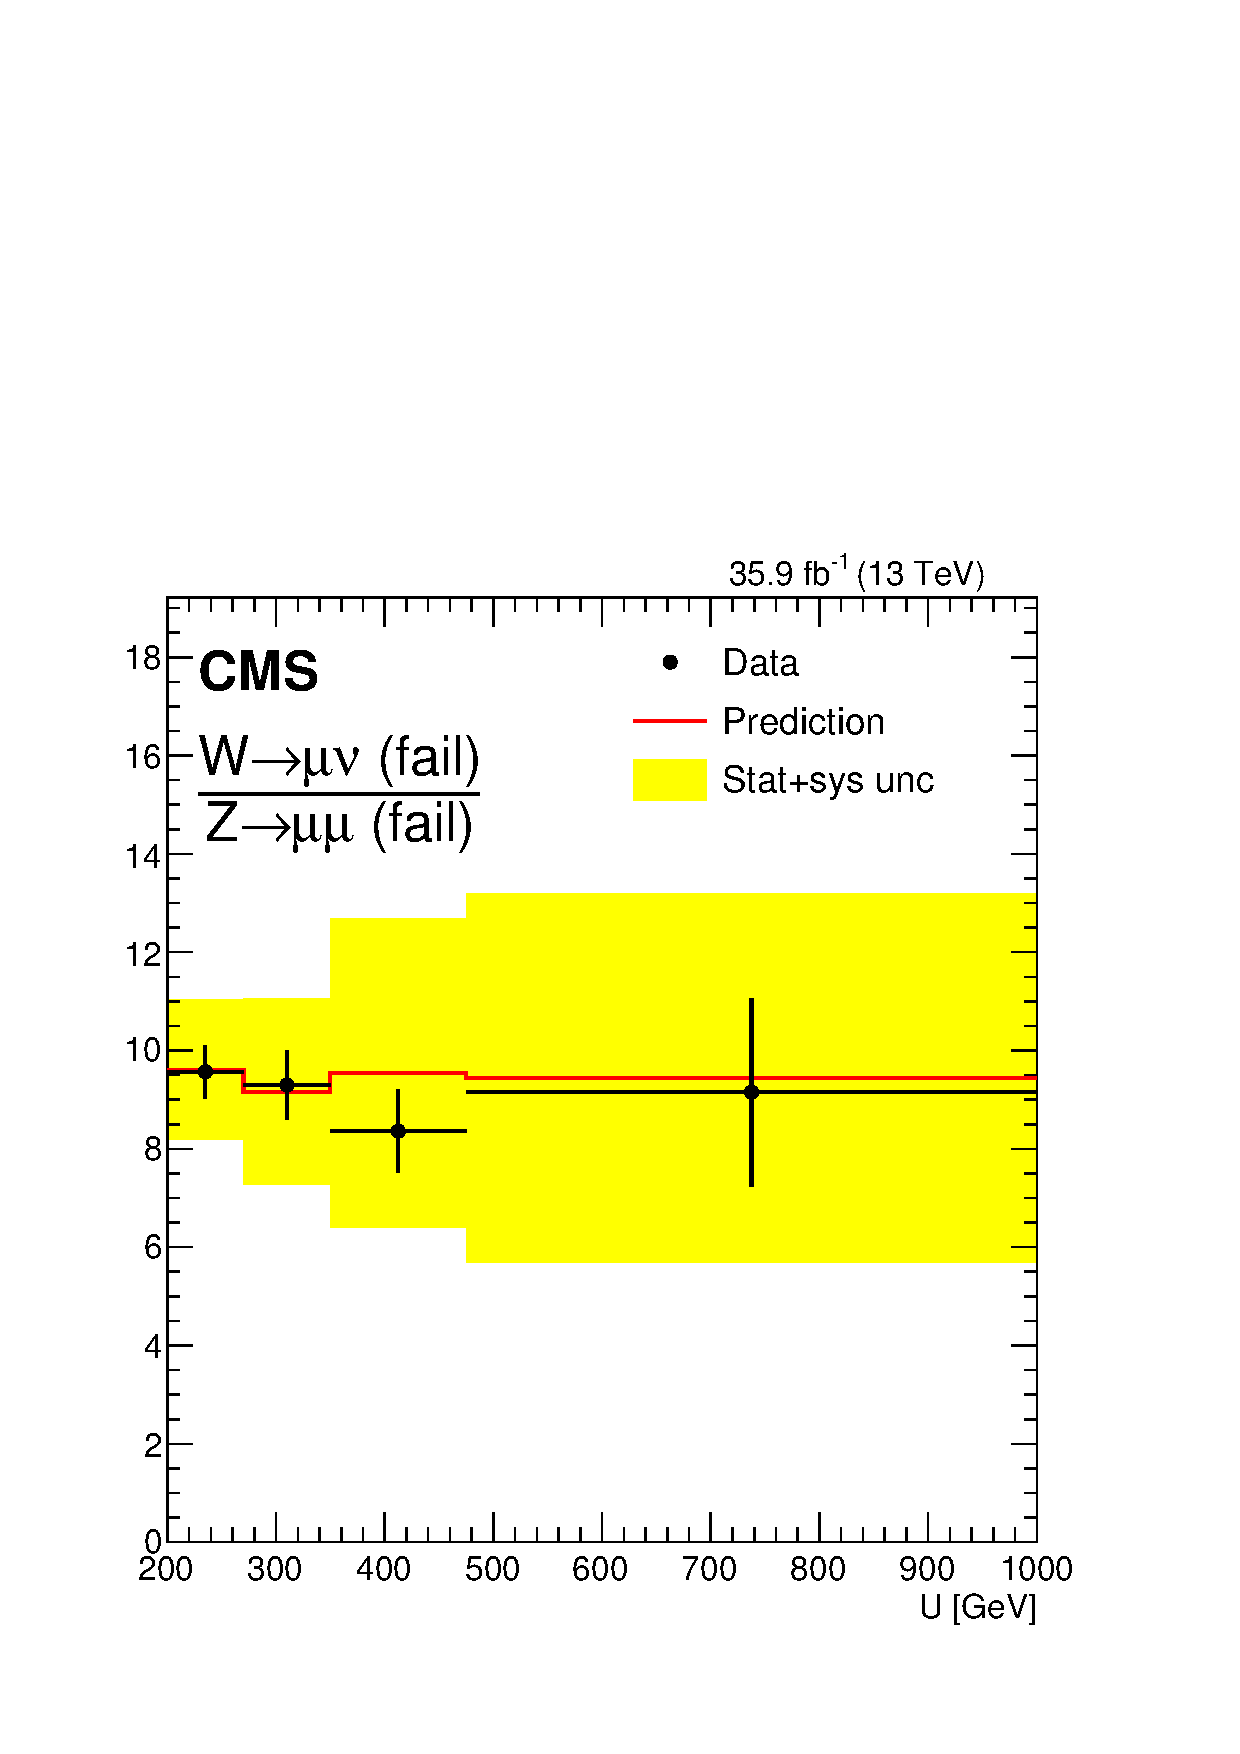
\includegraphics[width=0.45\textwidth]{figures/pullsImpact/ratio_wmn_fail_zmm_fail_shapes_prefit.pdf}
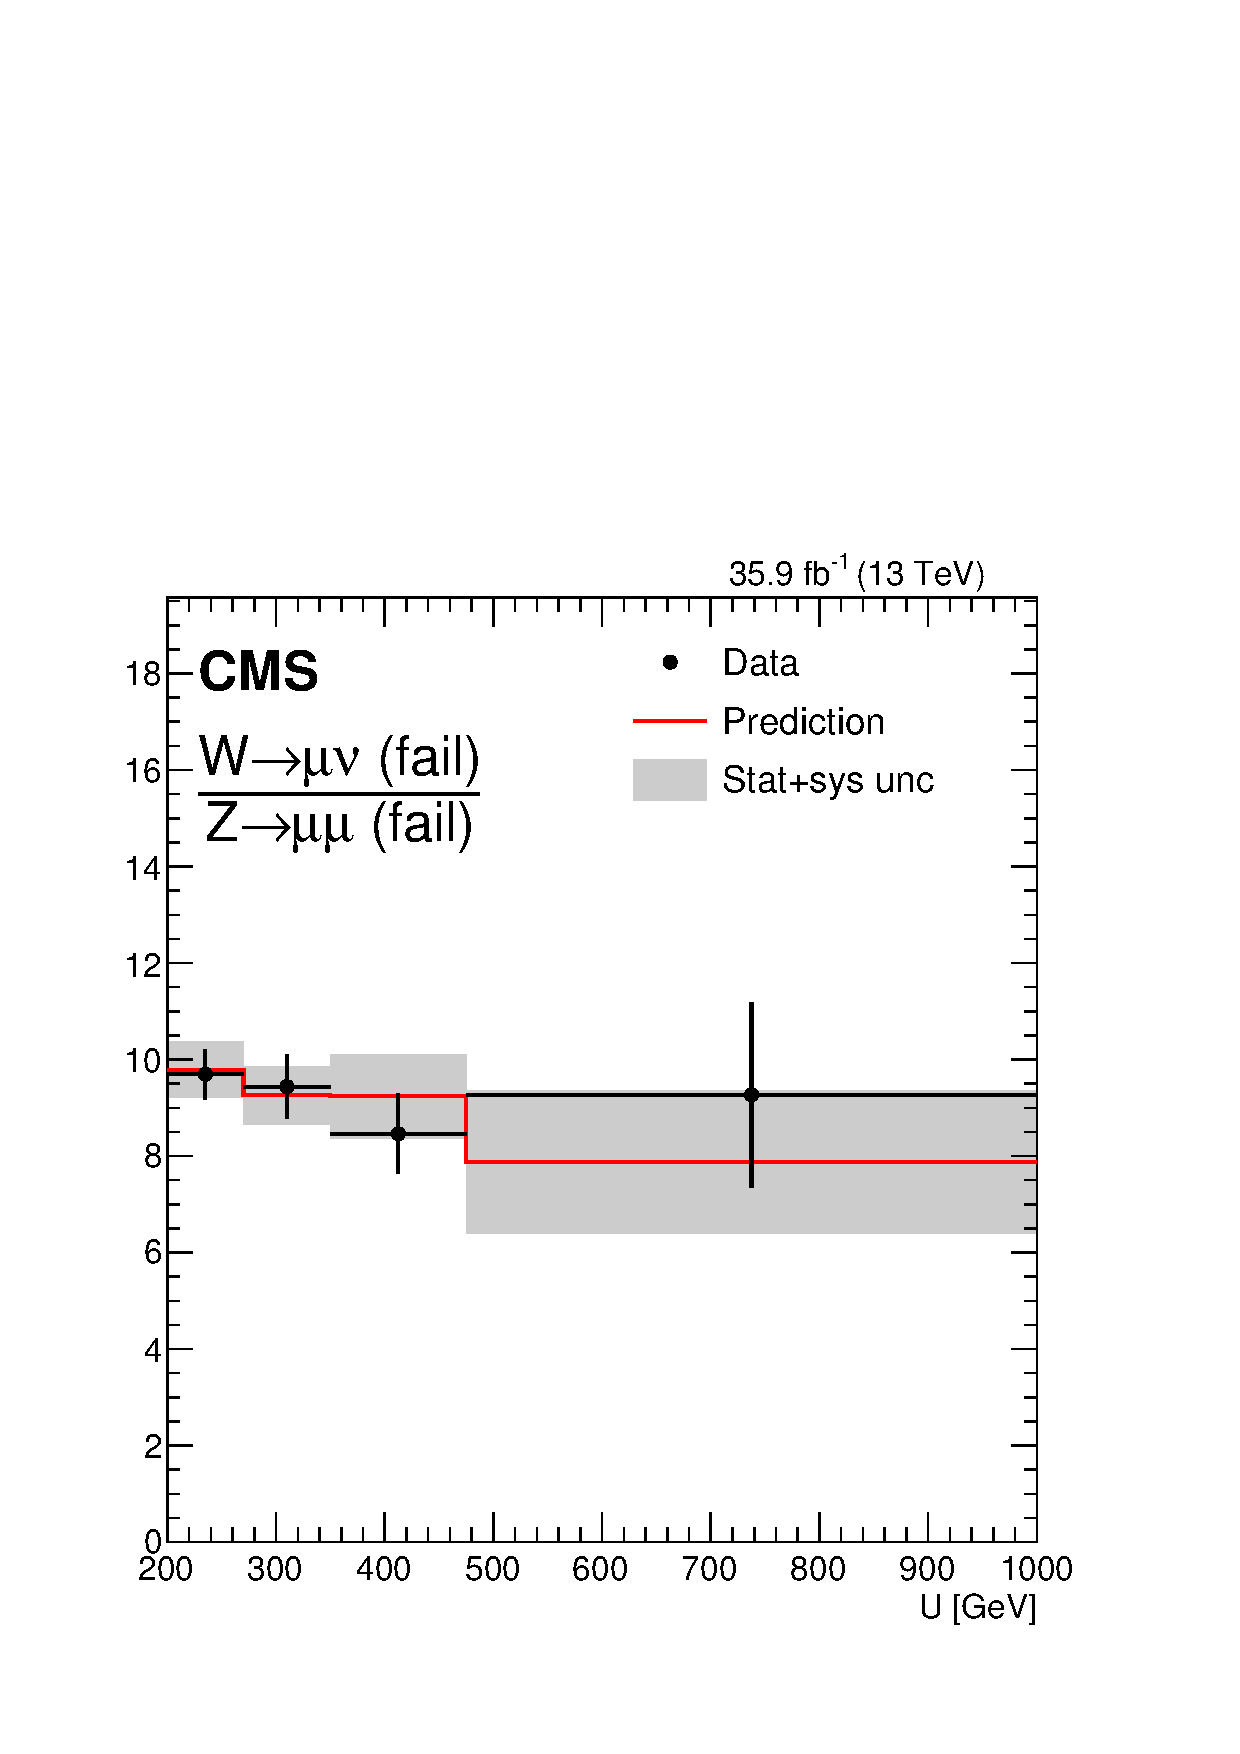
\includegraphics[width=0.45\textwidth]{figures/pullsImpact/ratio_wmn_fail_zmm_fail_shapes_fit_b.pdf}\\
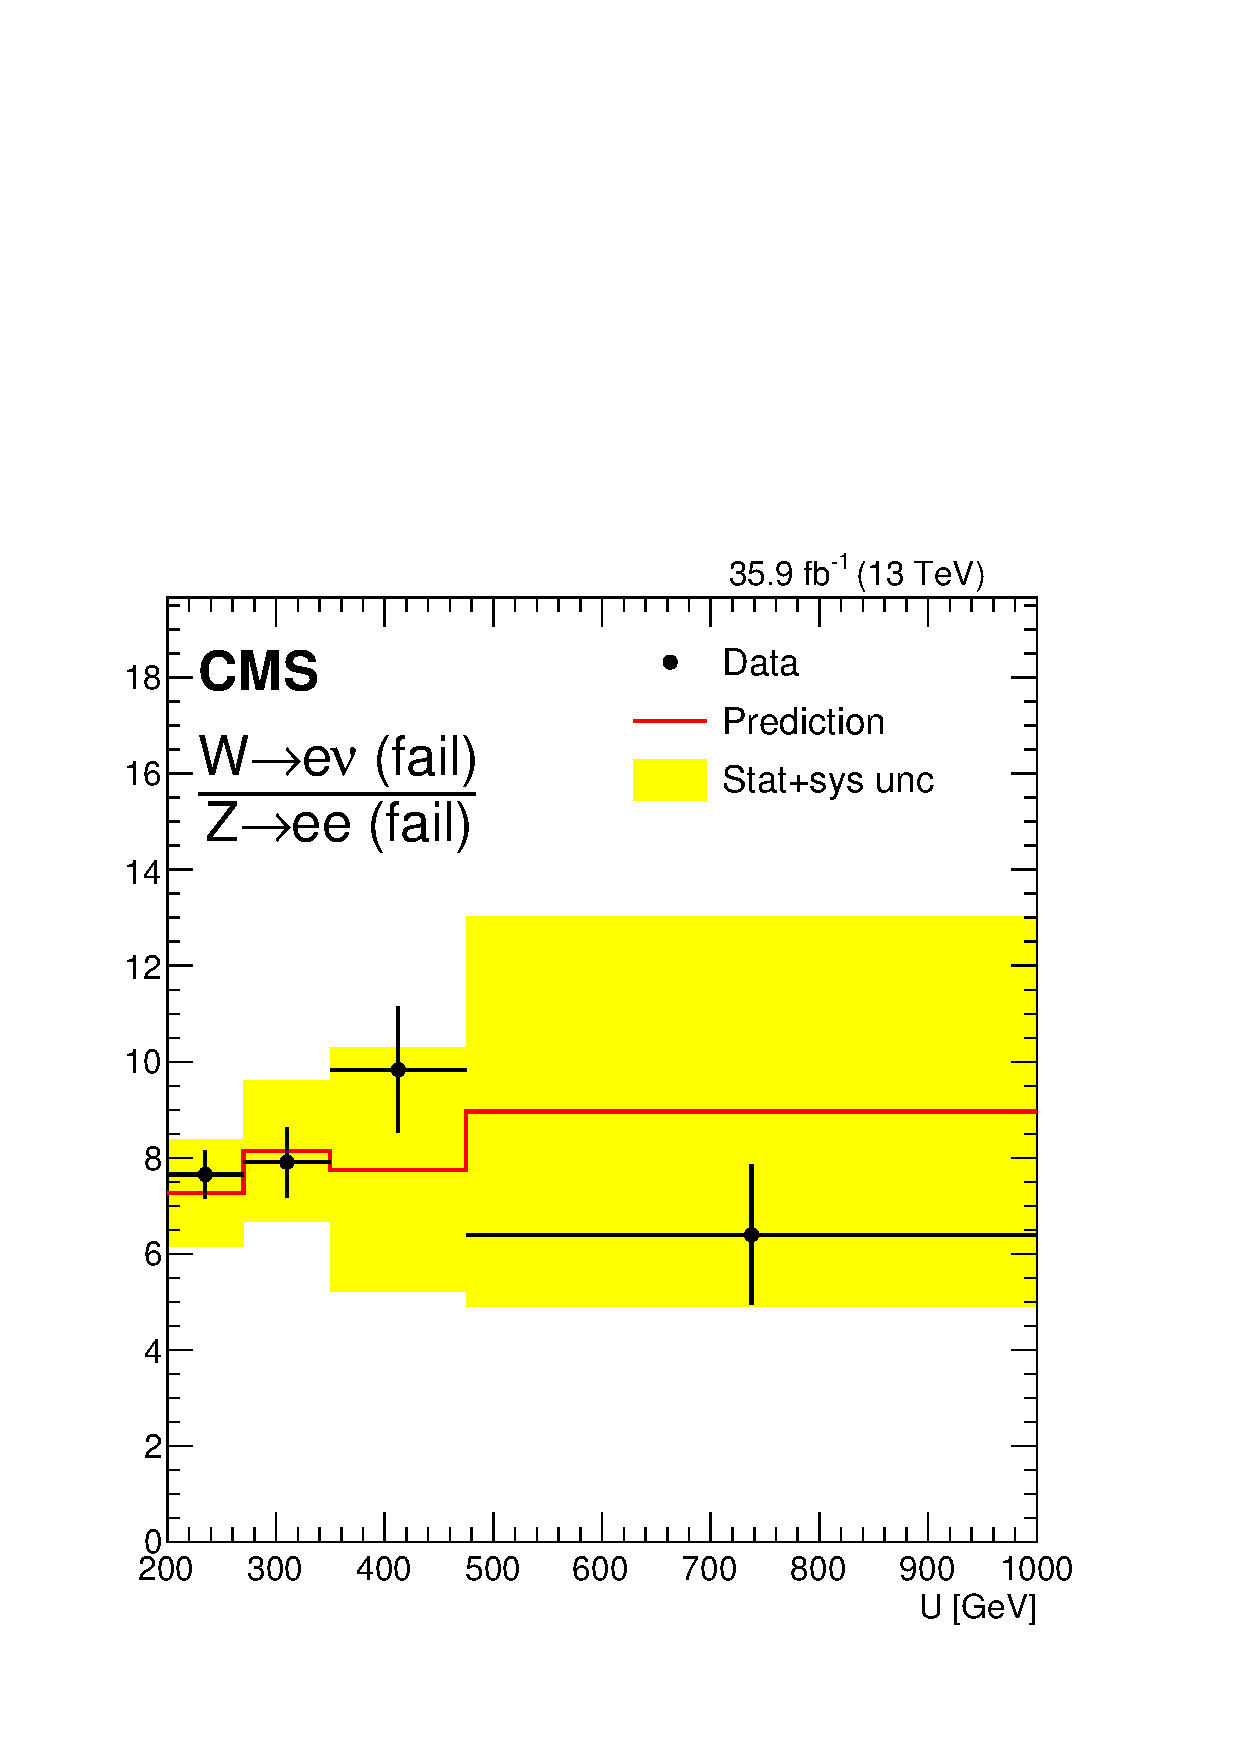
\includegraphics[width=0.45\textwidth]{figures/pullsImpact/ratio_wen_fail_zee_fail_shapes_prefit.pdf}
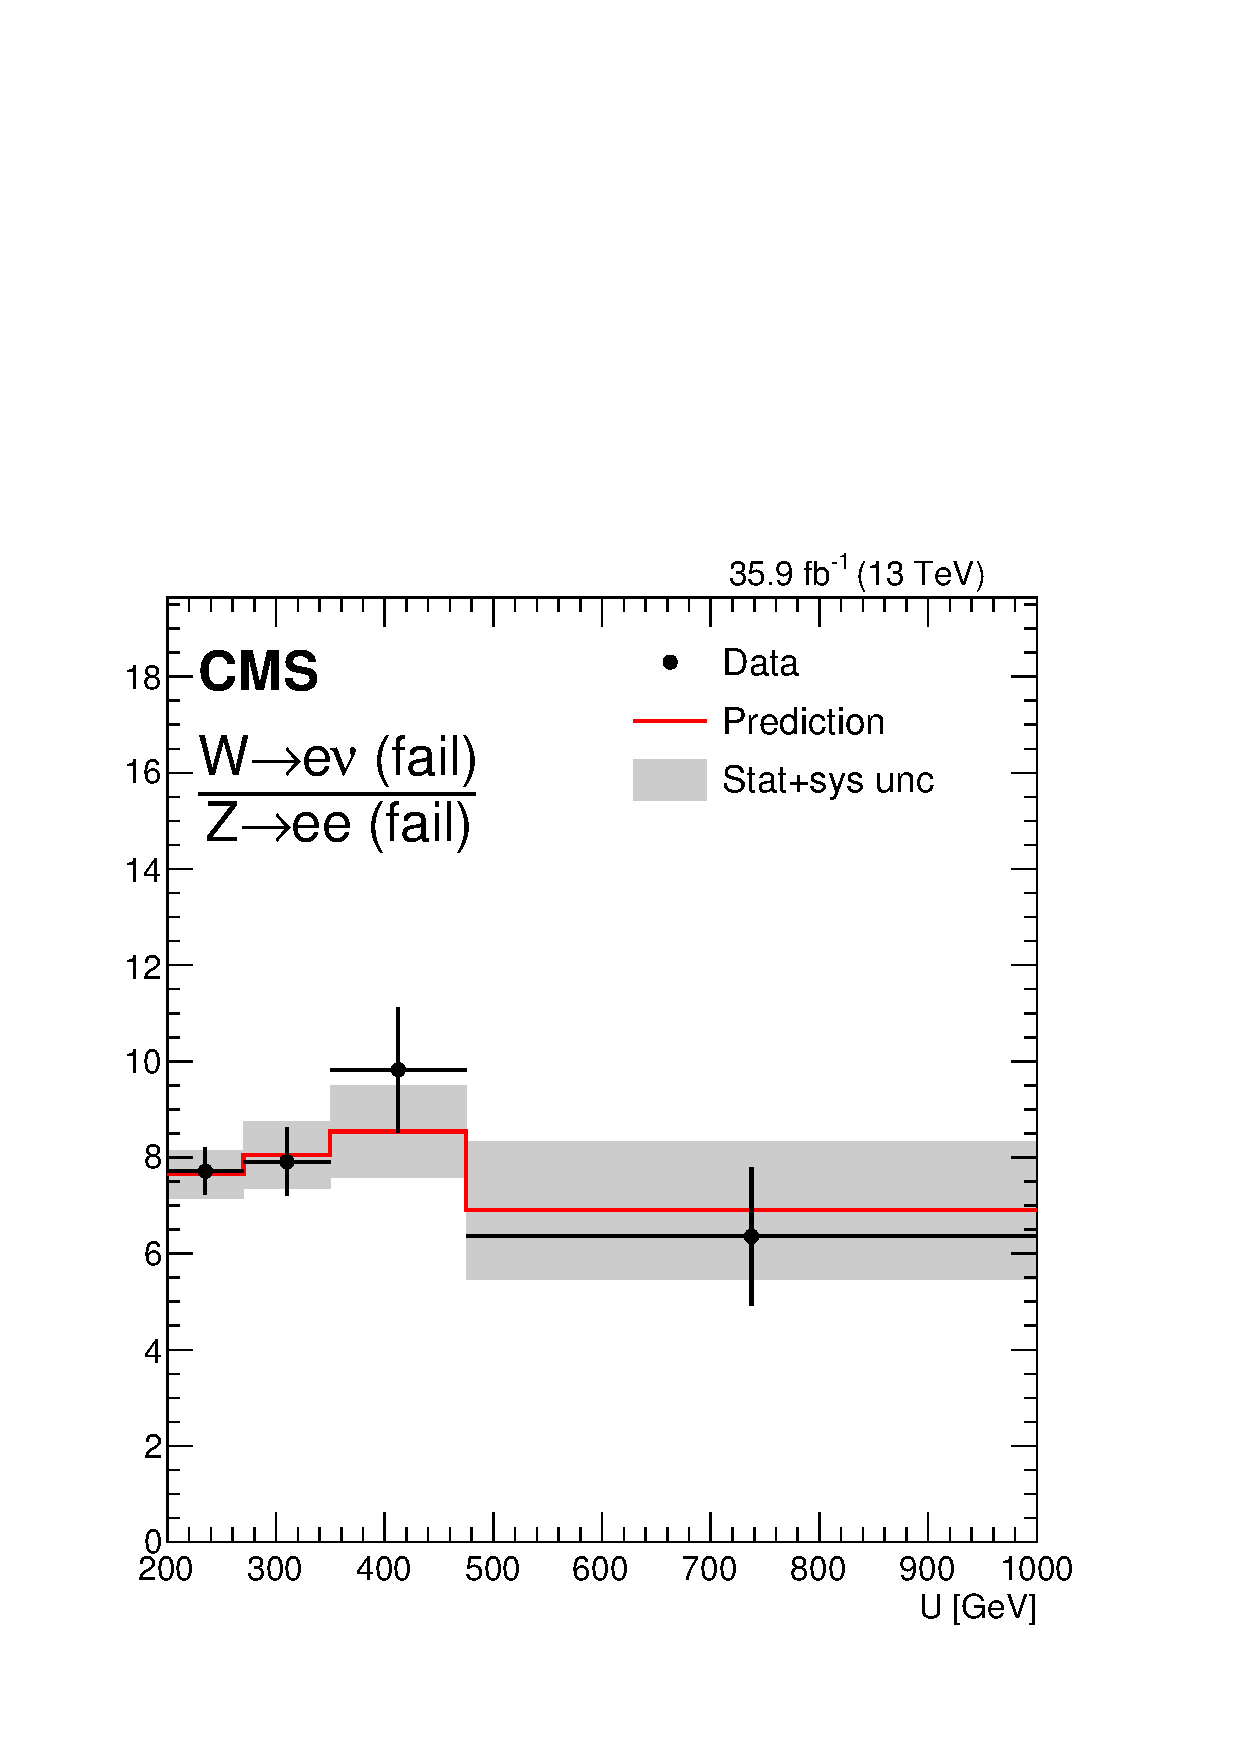
\includegraphics[width=0.45\textwidth]{figures/pullsImpact/ratio_wen_fail_zee_fail_shapes_fit_b.pdf}\\
\caption{Ratios of pre-fit (left column) and post-fit (right column) templates for W+jets and Z+jets processes in the W/Z fail regions. Black dots indicate the ratio of data yields (after subtracting trailing backgrounds) and demonstrate good agreement between data and simulation.}
\label{wzratios}
\end{figure}

\clearpage

\begin{figure}
\centering
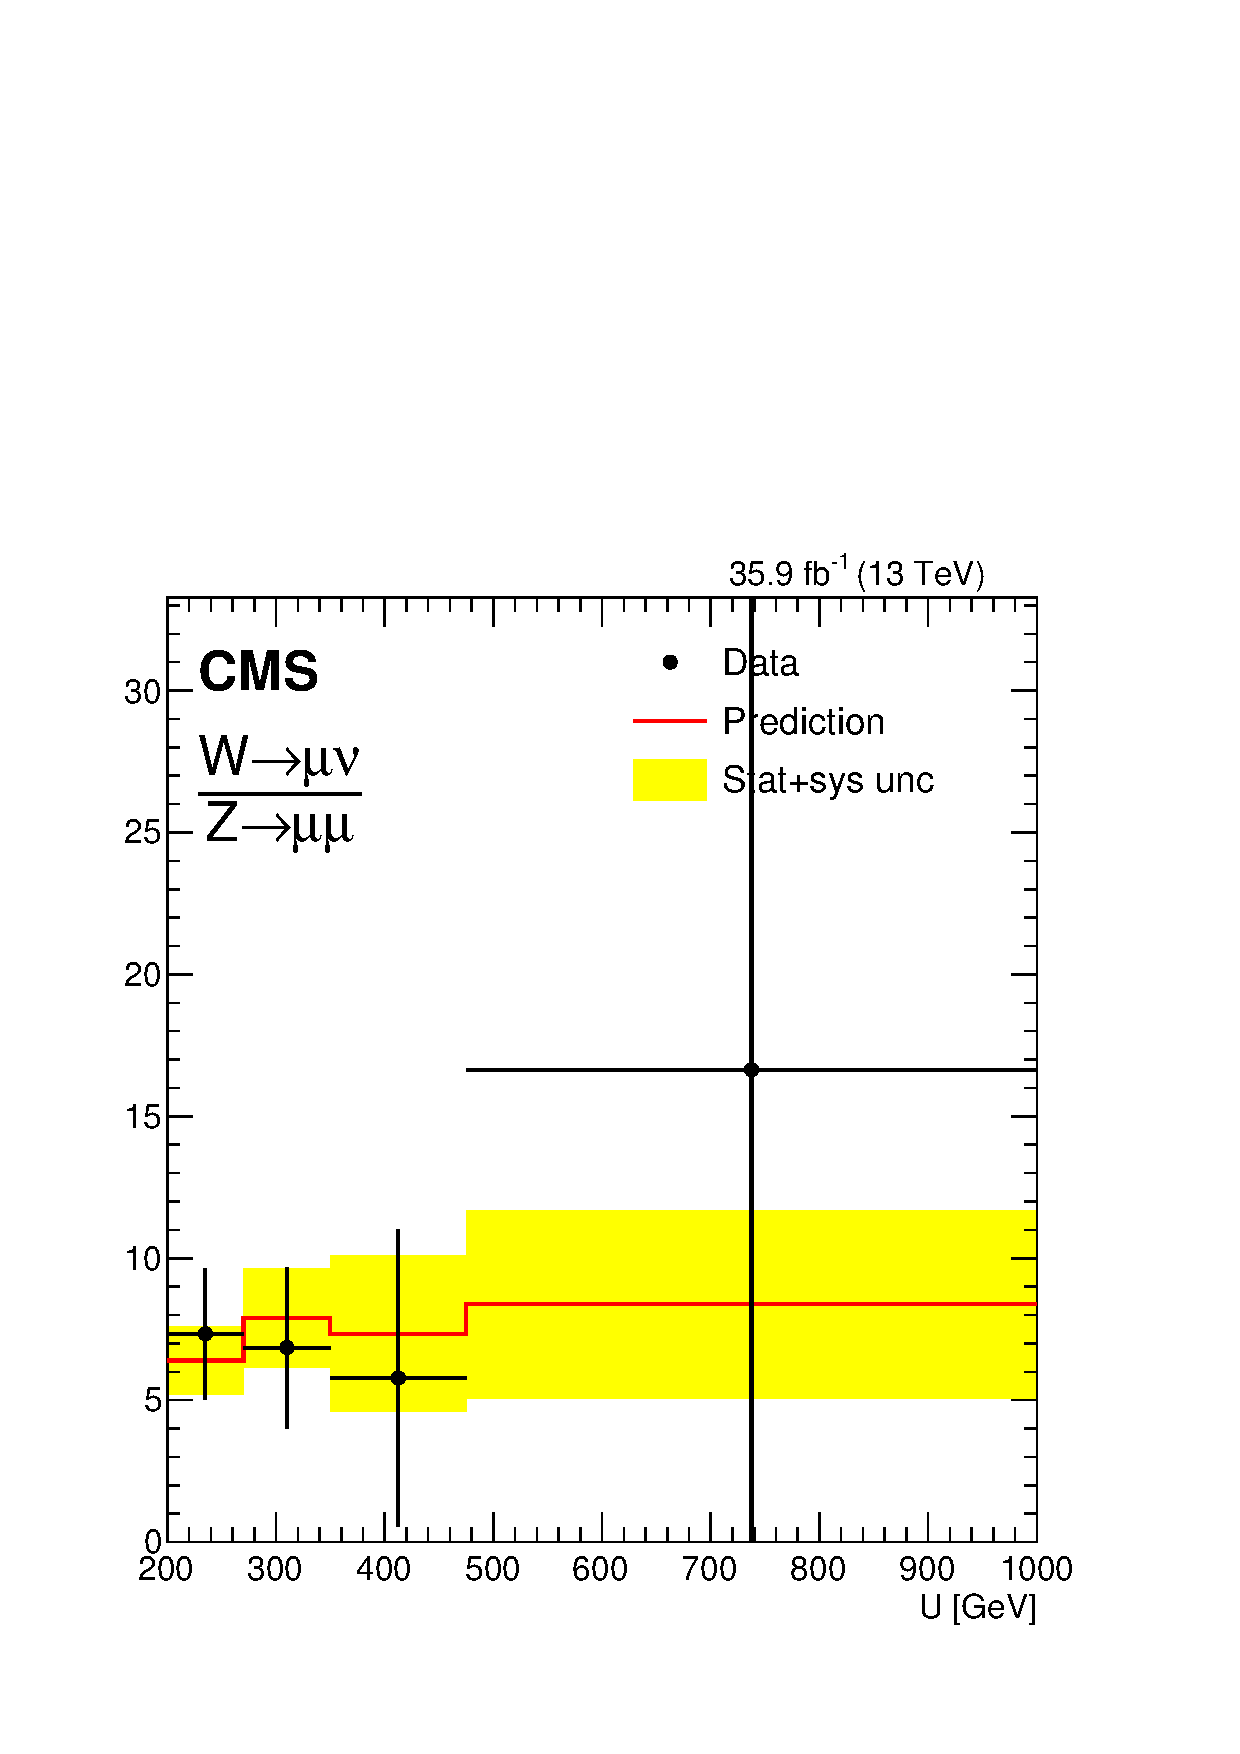
\includegraphics[width=0.45\textwidth]{figures/pullsImpact/ratio_wmn_zmm_shapes_prefit.pdf}
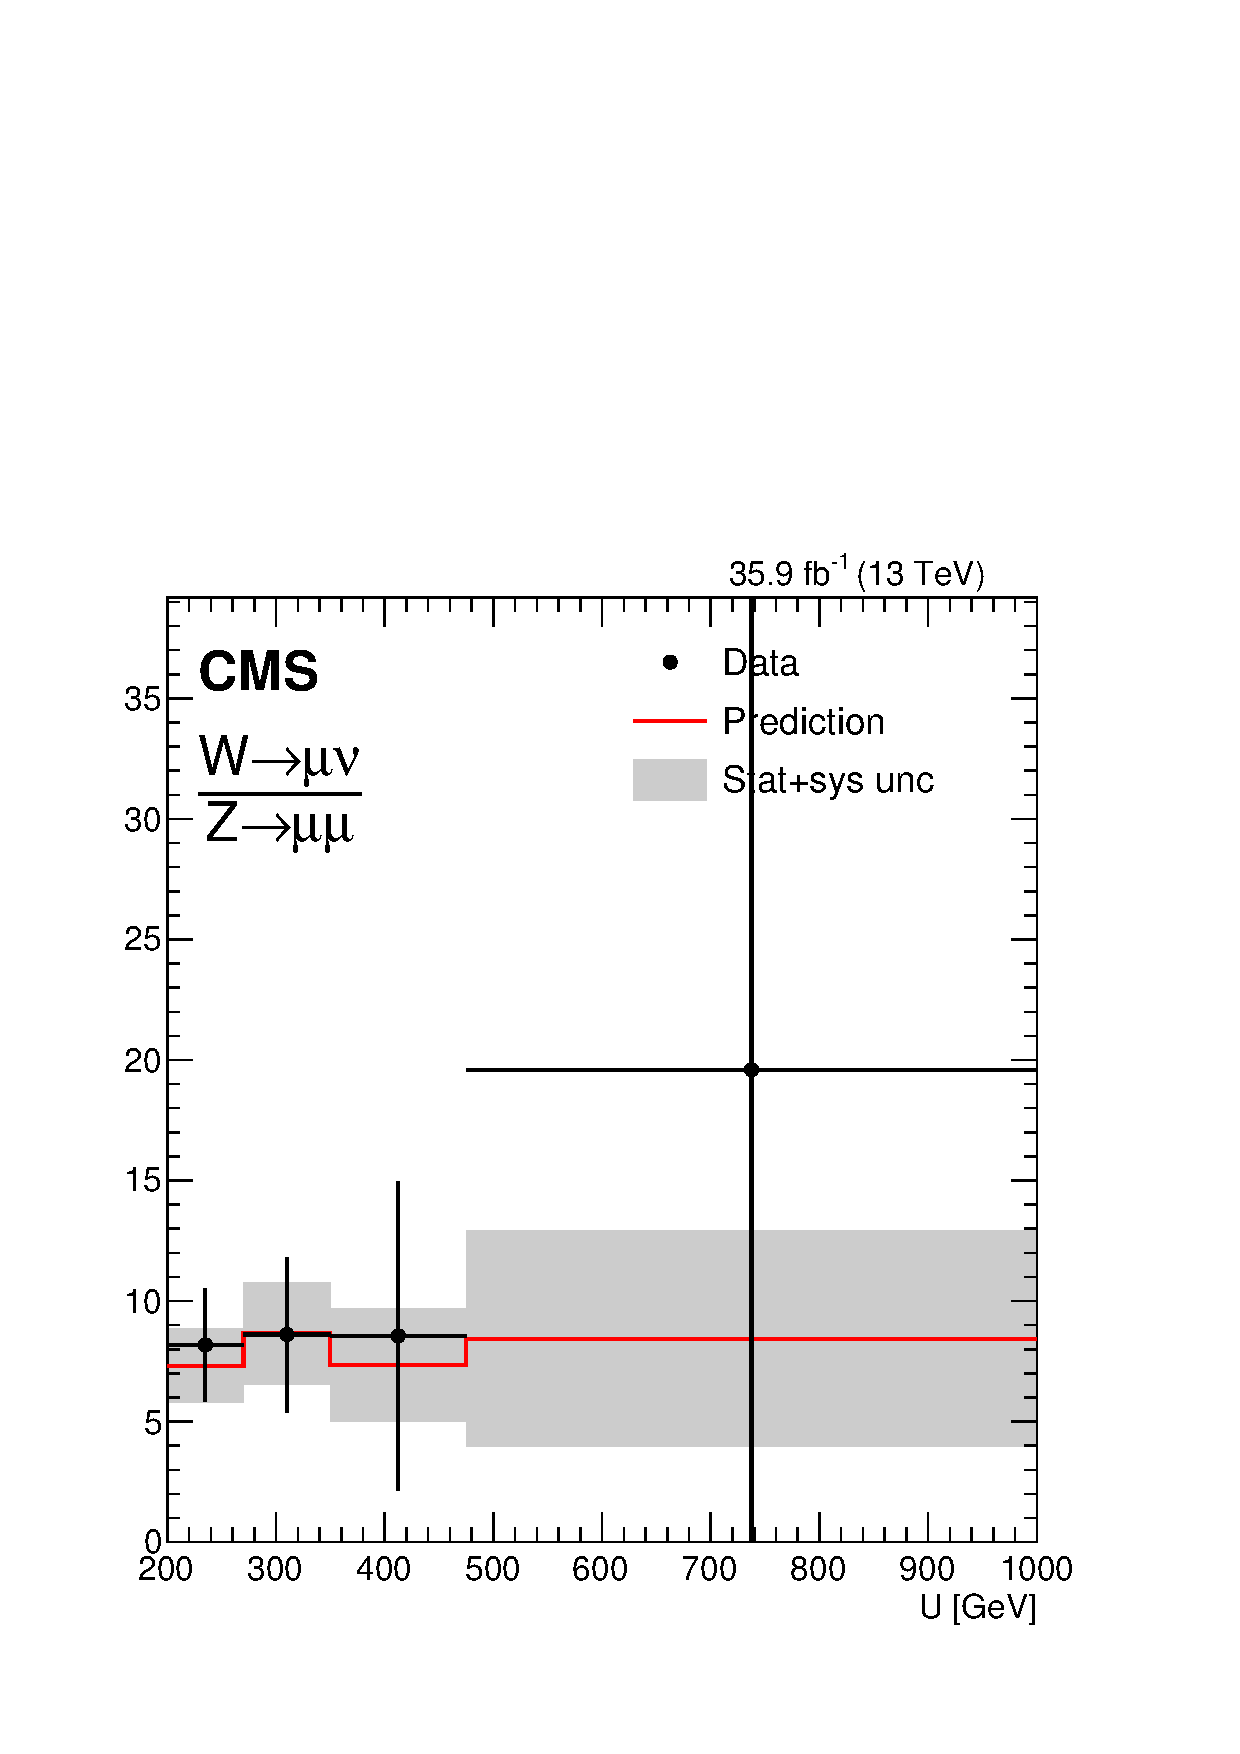
\includegraphics[width=0.45\textwidth]{figures/pullsImpact/ratio_wmn_zmm_shapes_fit_b.pdf}\\
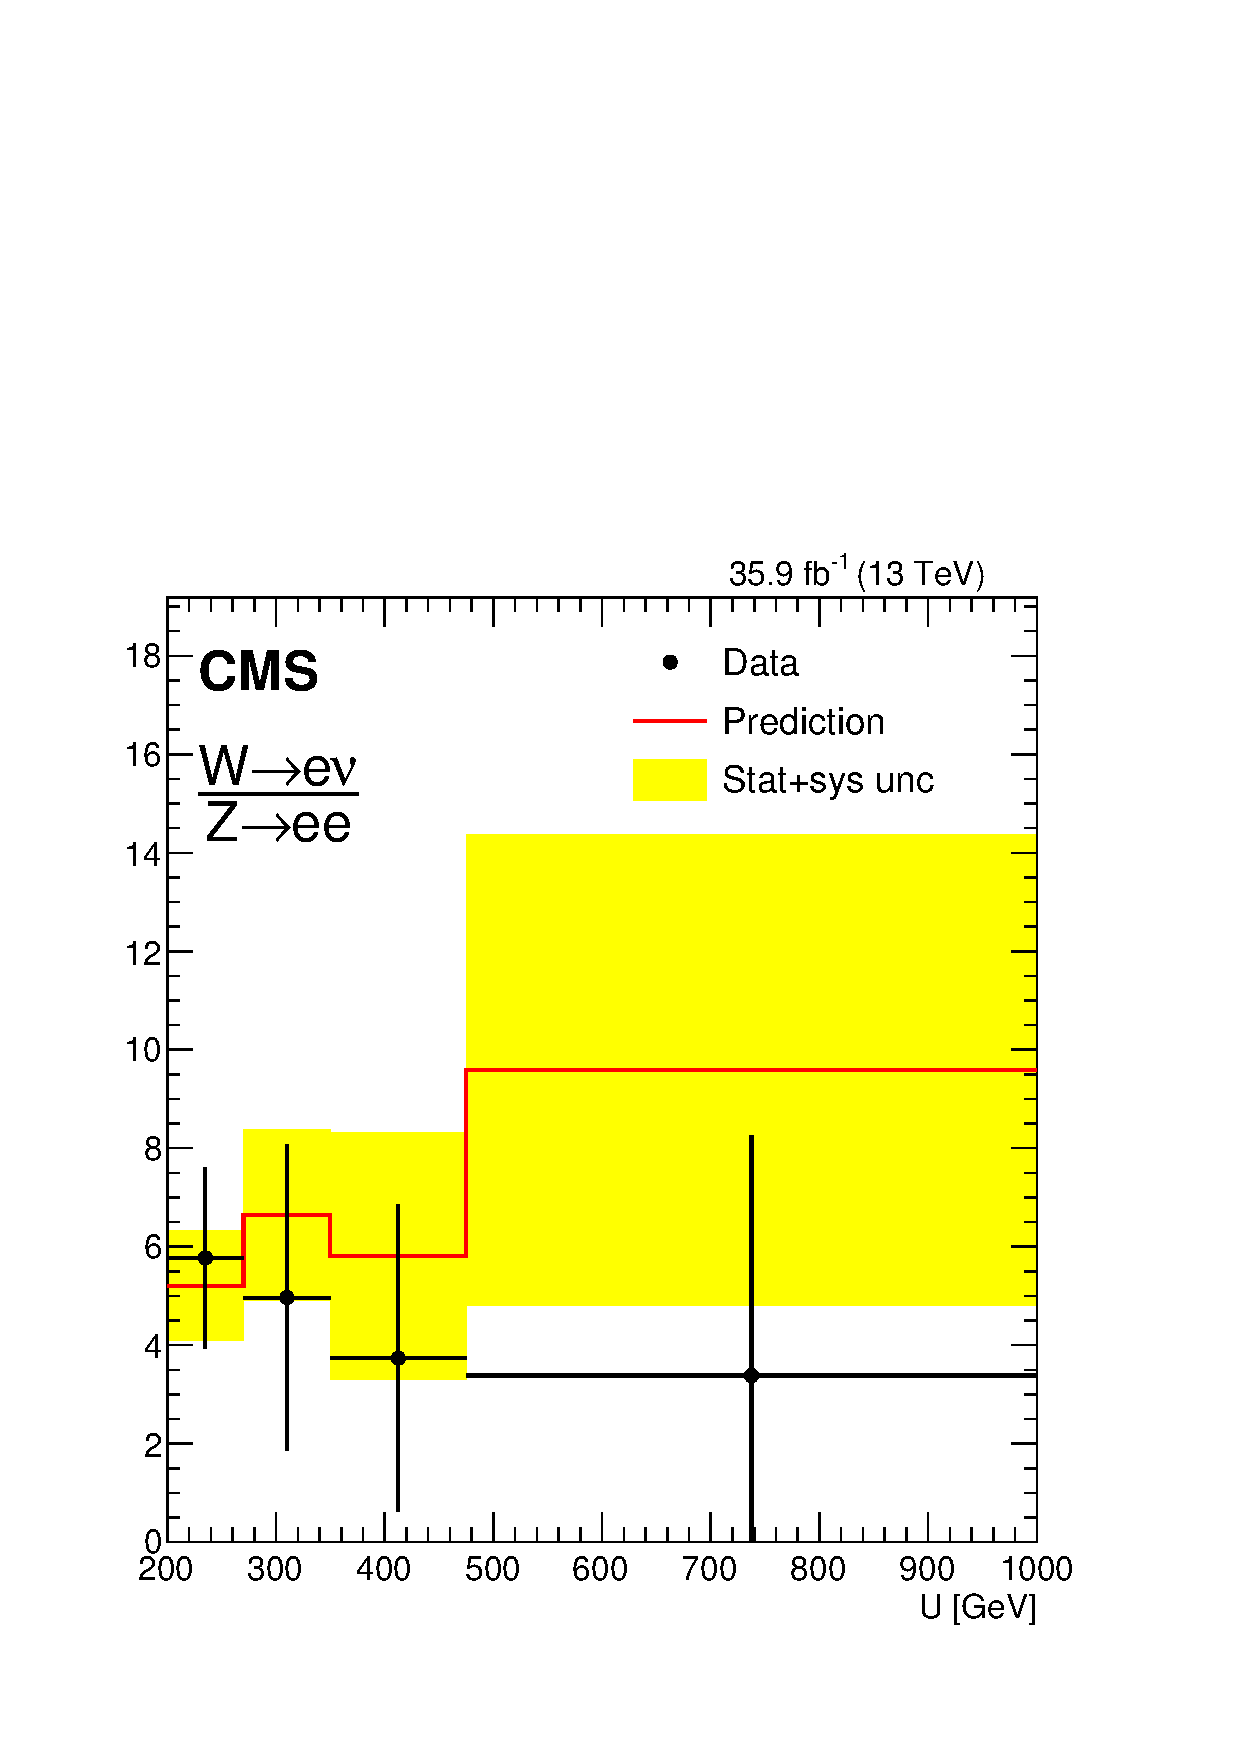
\includegraphics[width=0.45\textwidth]{figures/pullsImpact/ratio_wen_zee_shapes_prefit.pdf}
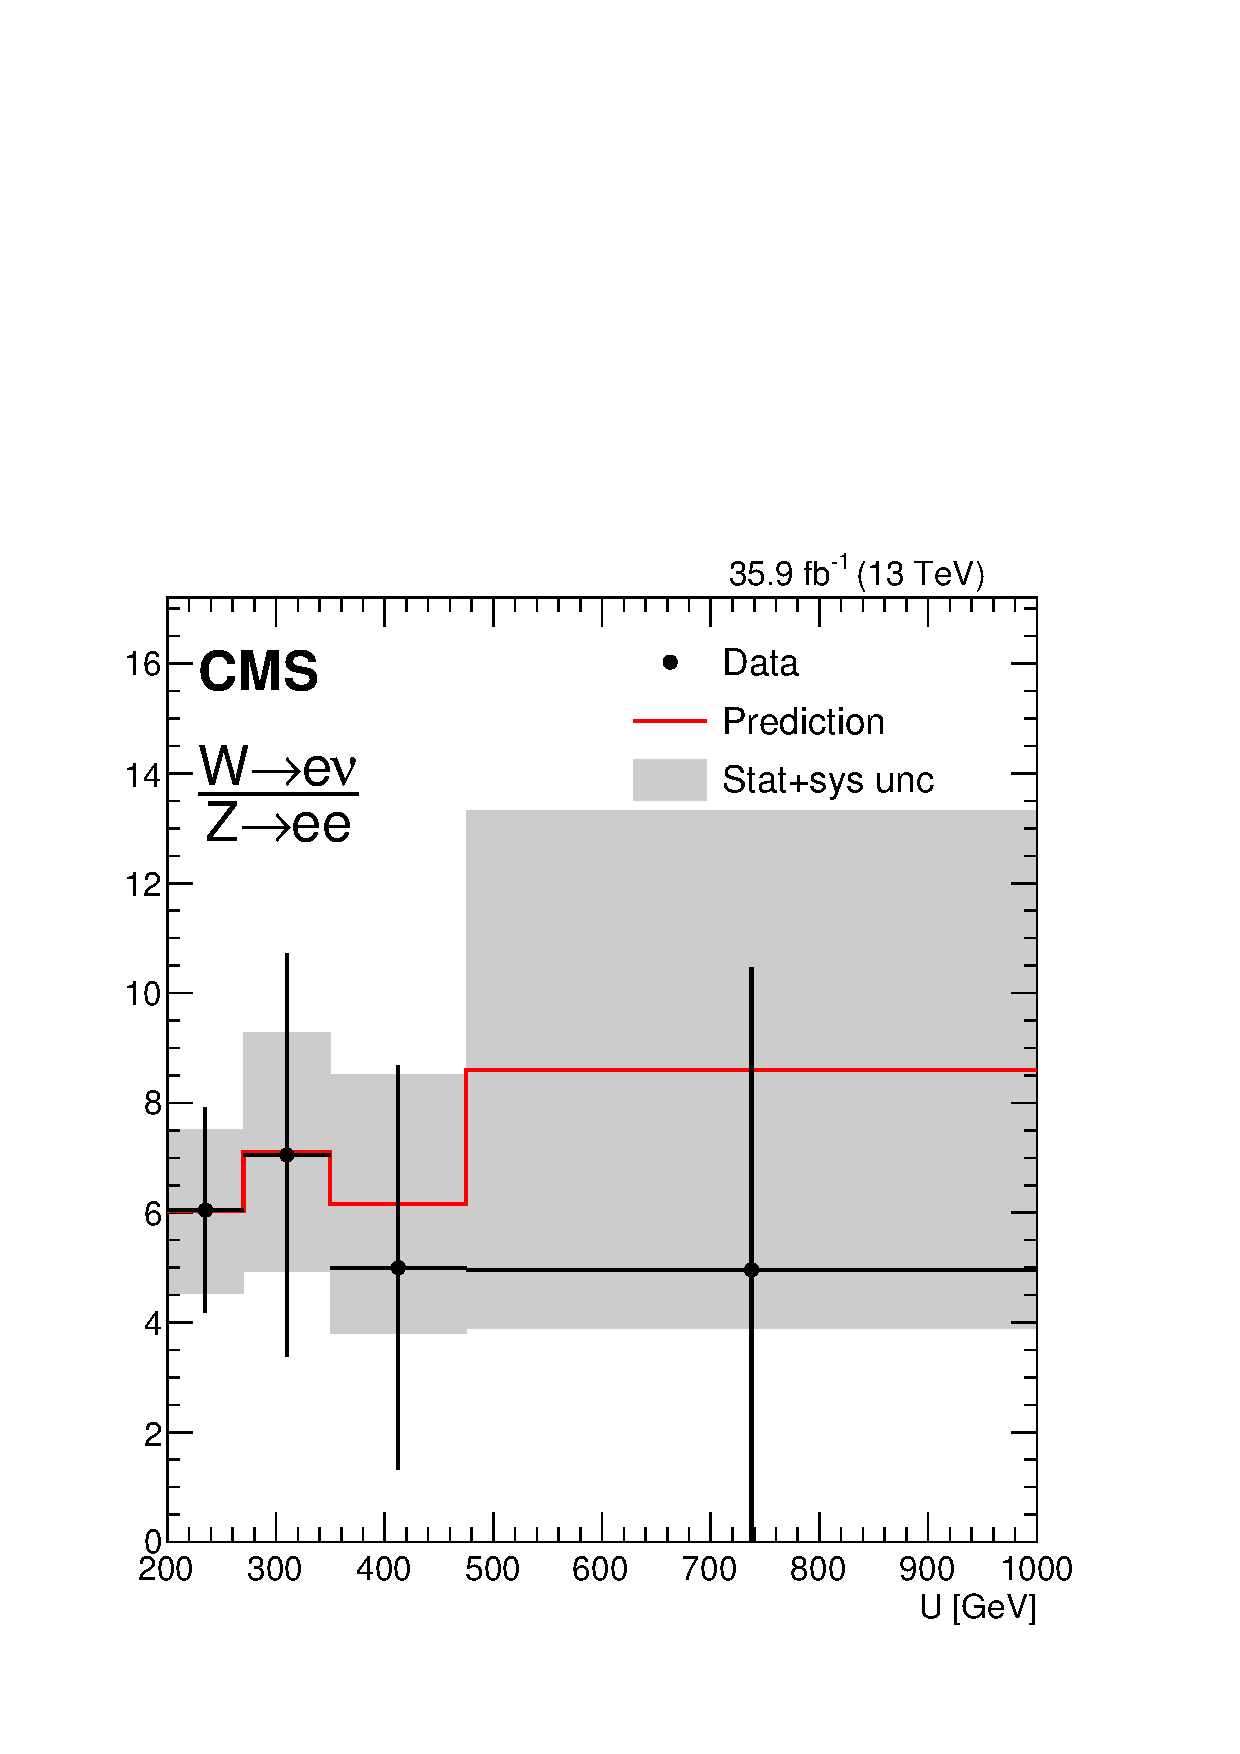
\includegraphics[width=0.45\textwidth]{figures/pullsImpact/ratio_wen_zee_shapes_fit_b.pdf}\\
\caption{Ratios of pre-fit (left column) and post-fit (right column) templates for W+jets and Z+jets processes in the W/Z pass regions. Black dots indicate the ratio of data yields (after subtracting trailing backgrounds) and demonstrate good agreement between data and simulation.}
\label{wzratios2}
\end{figure}

\clearpage

\begin{figure}
\centering
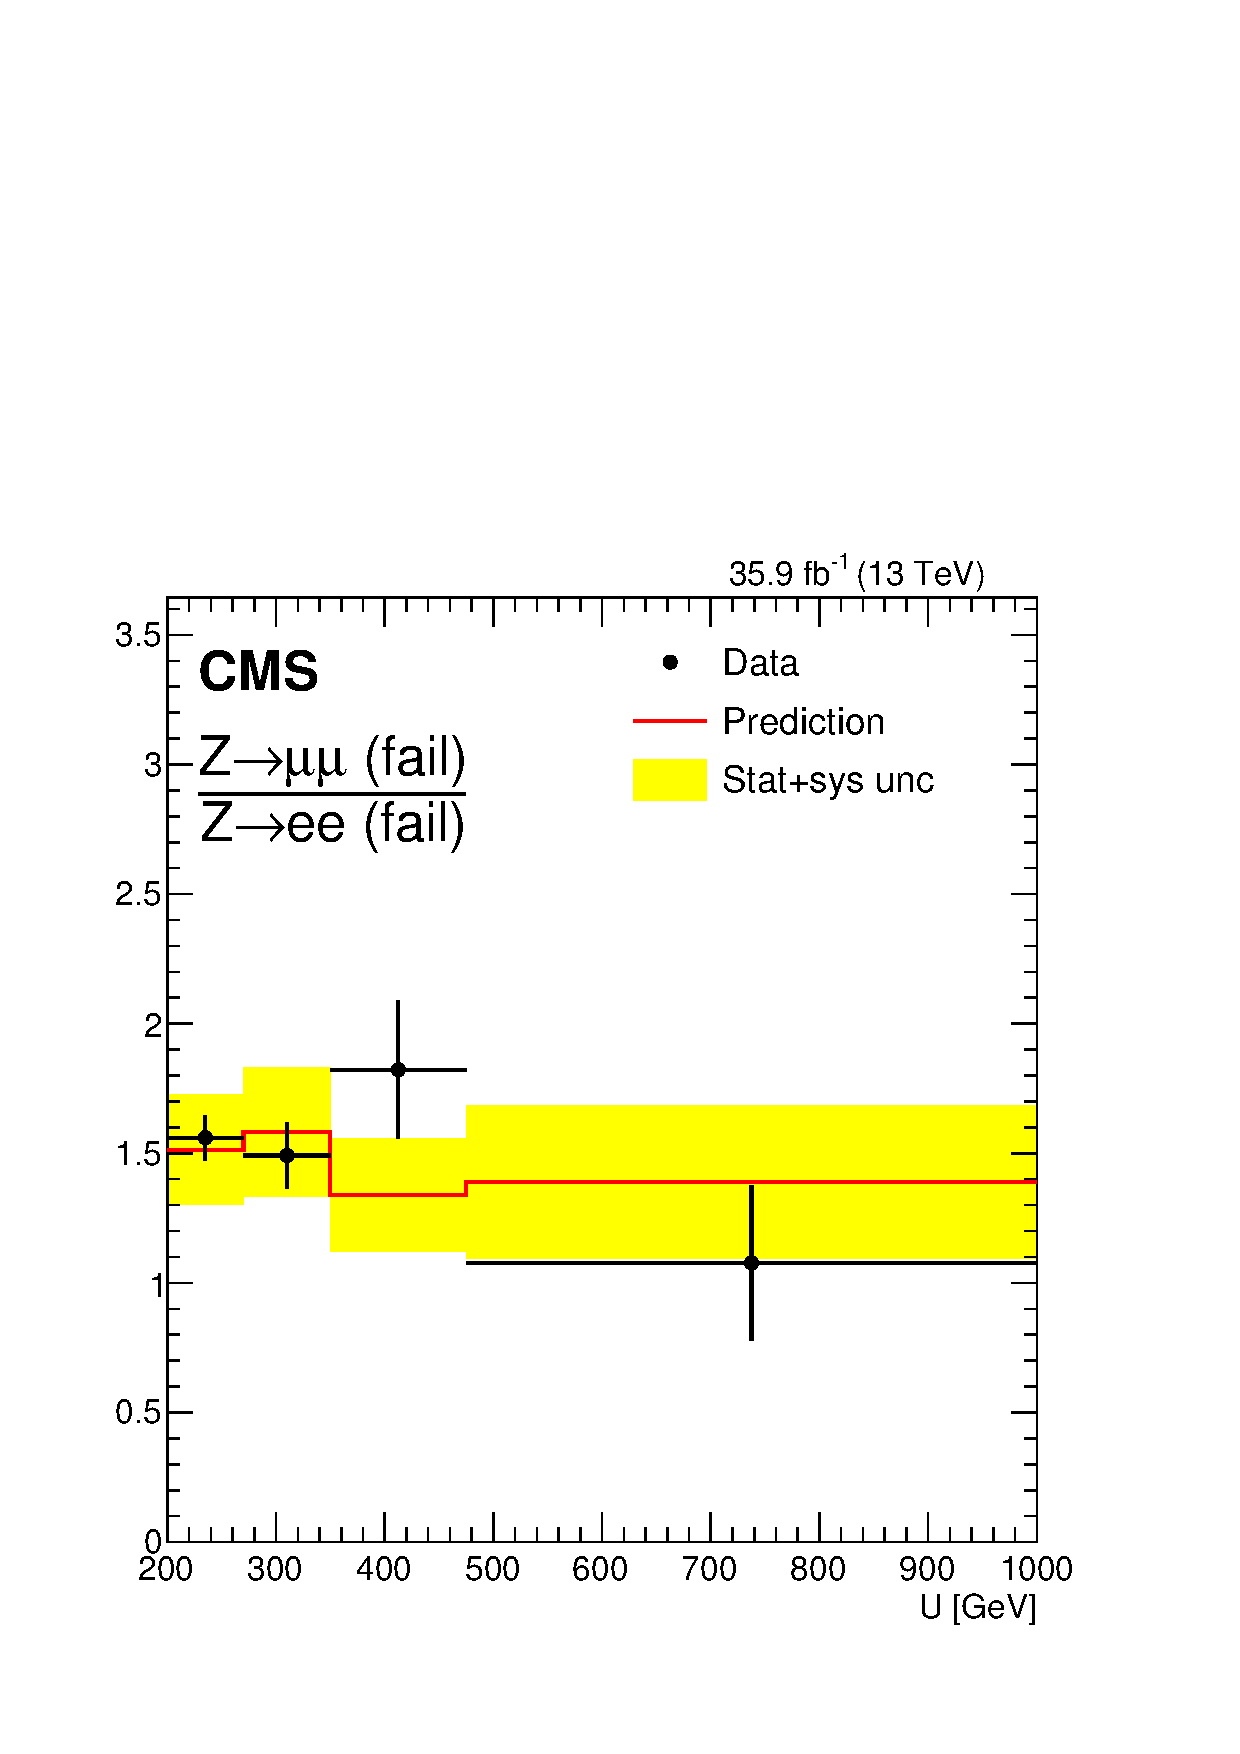
\includegraphics[width=0.45\textwidth]{figures/pullsImpact/ratio_zmm_fail_zee_fail_shapes_prefit.pdf}
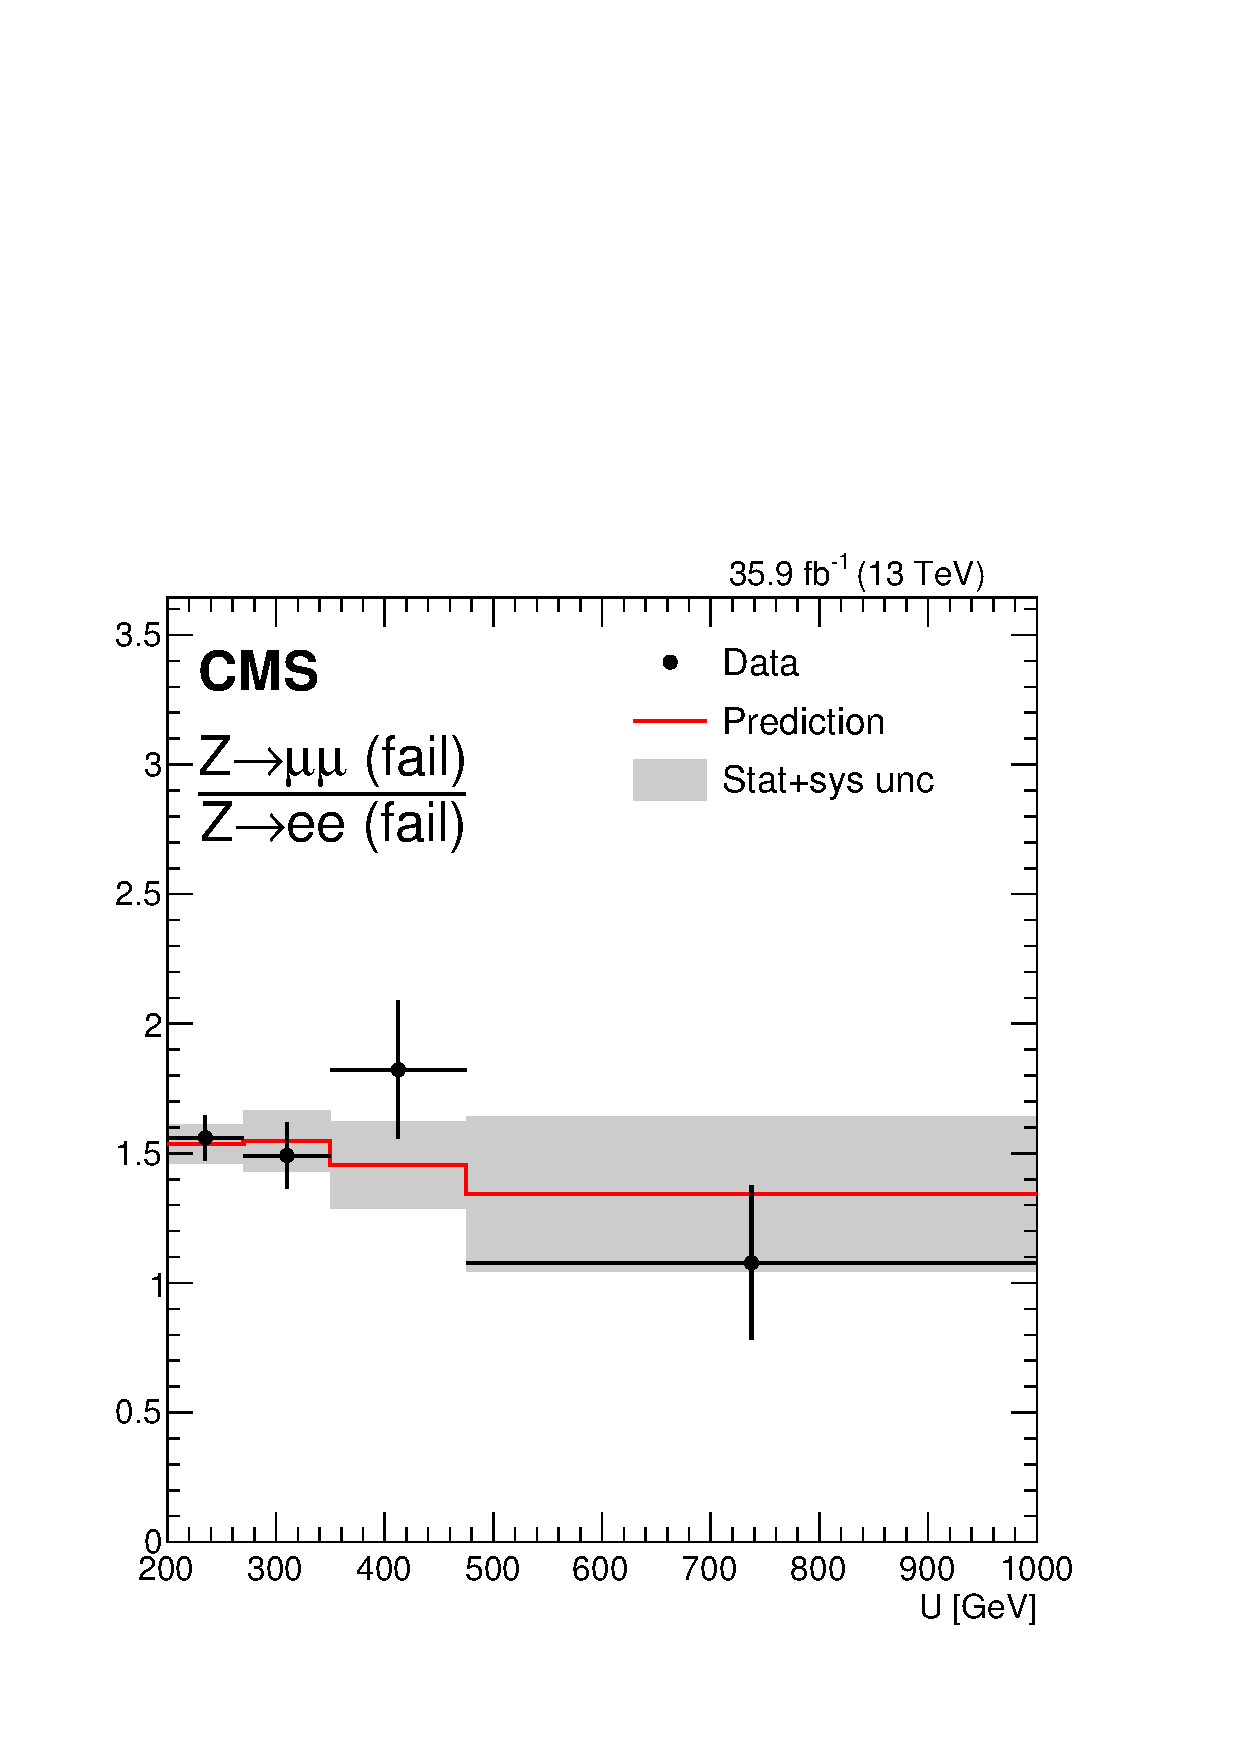
\includegraphics[width=0.45\textwidth]{figures/pullsImpact/ratio_zmm_fail_zee_fail_shapes_fit_b.pdf}\\
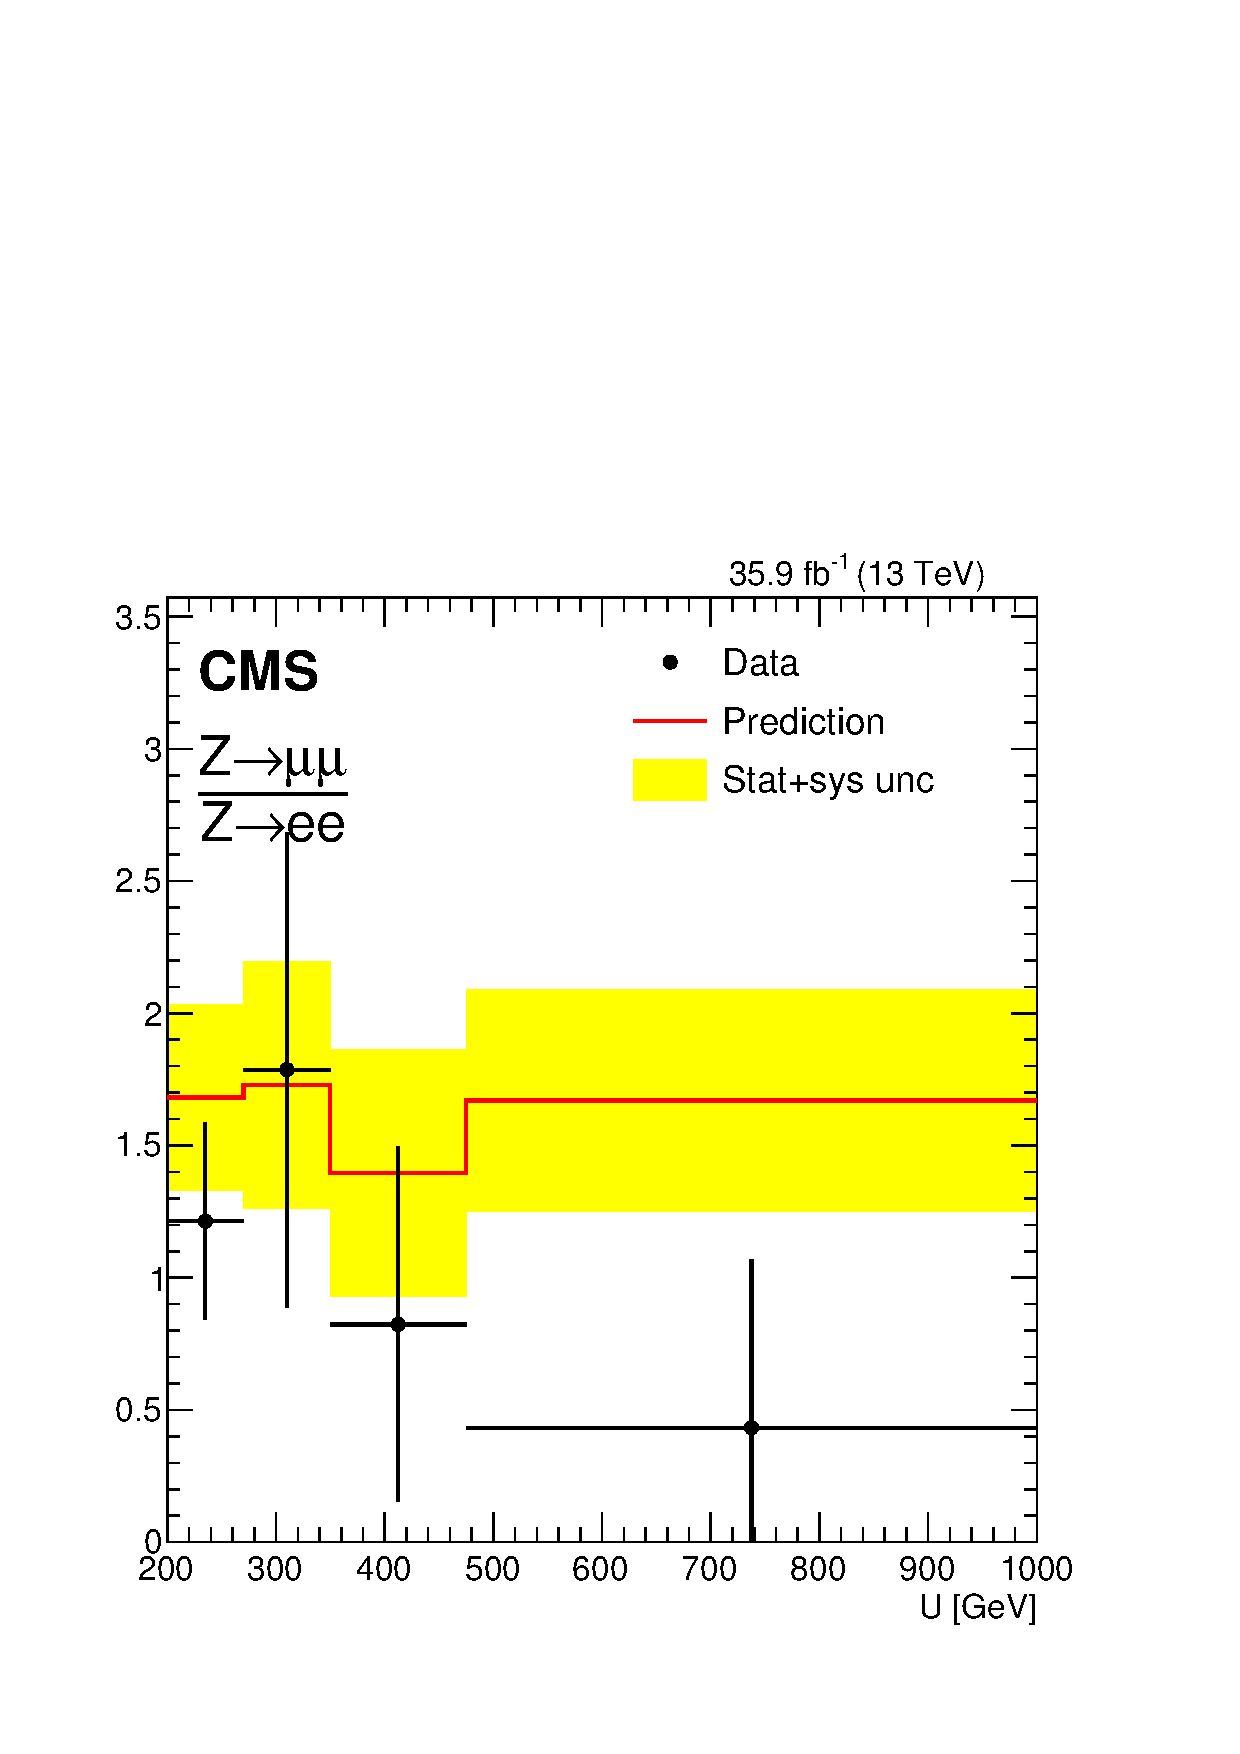
\includegraphics[width=0.45\textwidth]{figures/pullsImpact/ratio_zmm_zee_shapes_prefit.pdf}
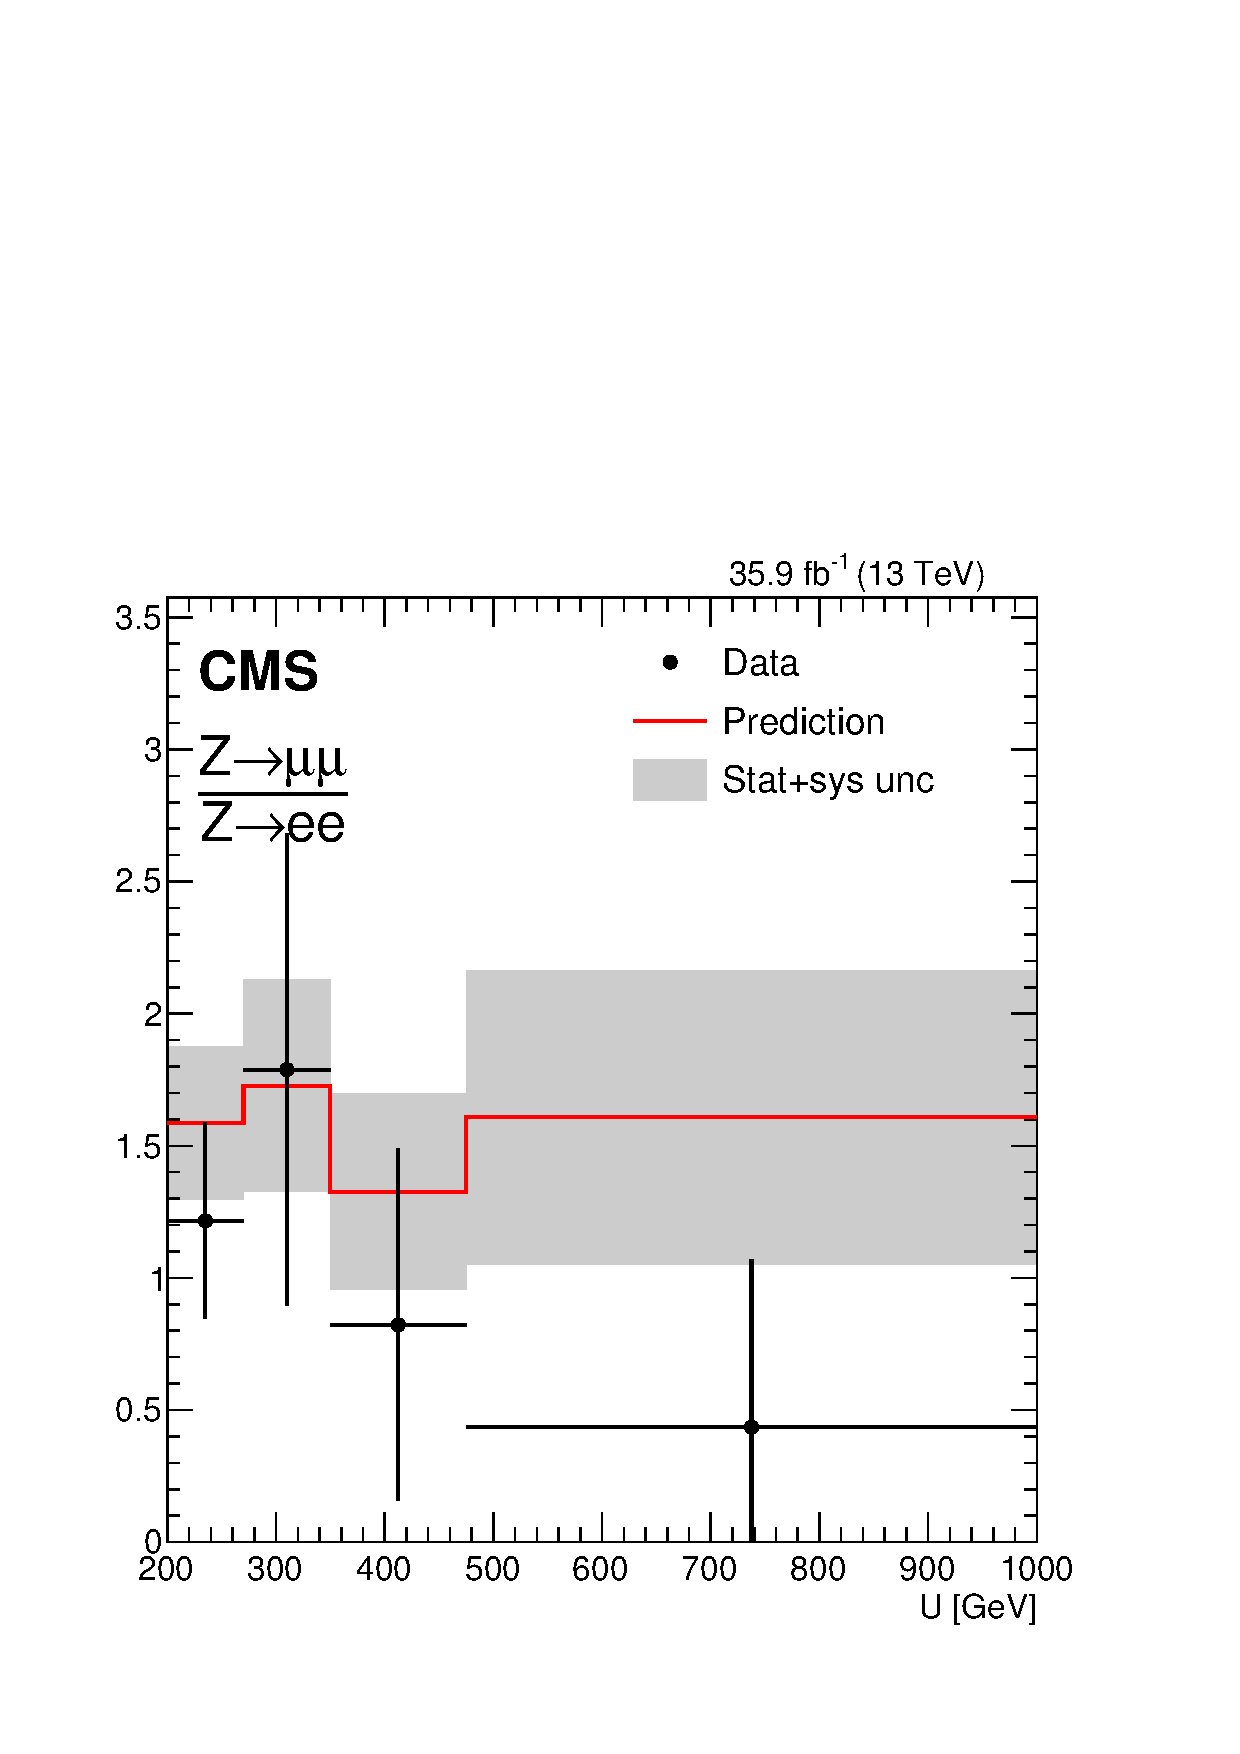
\includegraphics[width=0.45\textwidth]{figures/pullsImpact/ratio_zmm_zee_shapes_fit_b.pdf}\\
\caption{Ratios of pre-fit (left column) and post-fit (right column) templates for Z+jets processes in the Z pass/fail regions. Black dots indicate the ratio of data yields (after subtracting trailing backgrounds) and demonstrate good agreement between data and simulation.}
\label{wwratios}
\end{figure}

\clearpage

\begin{figure}
\centering
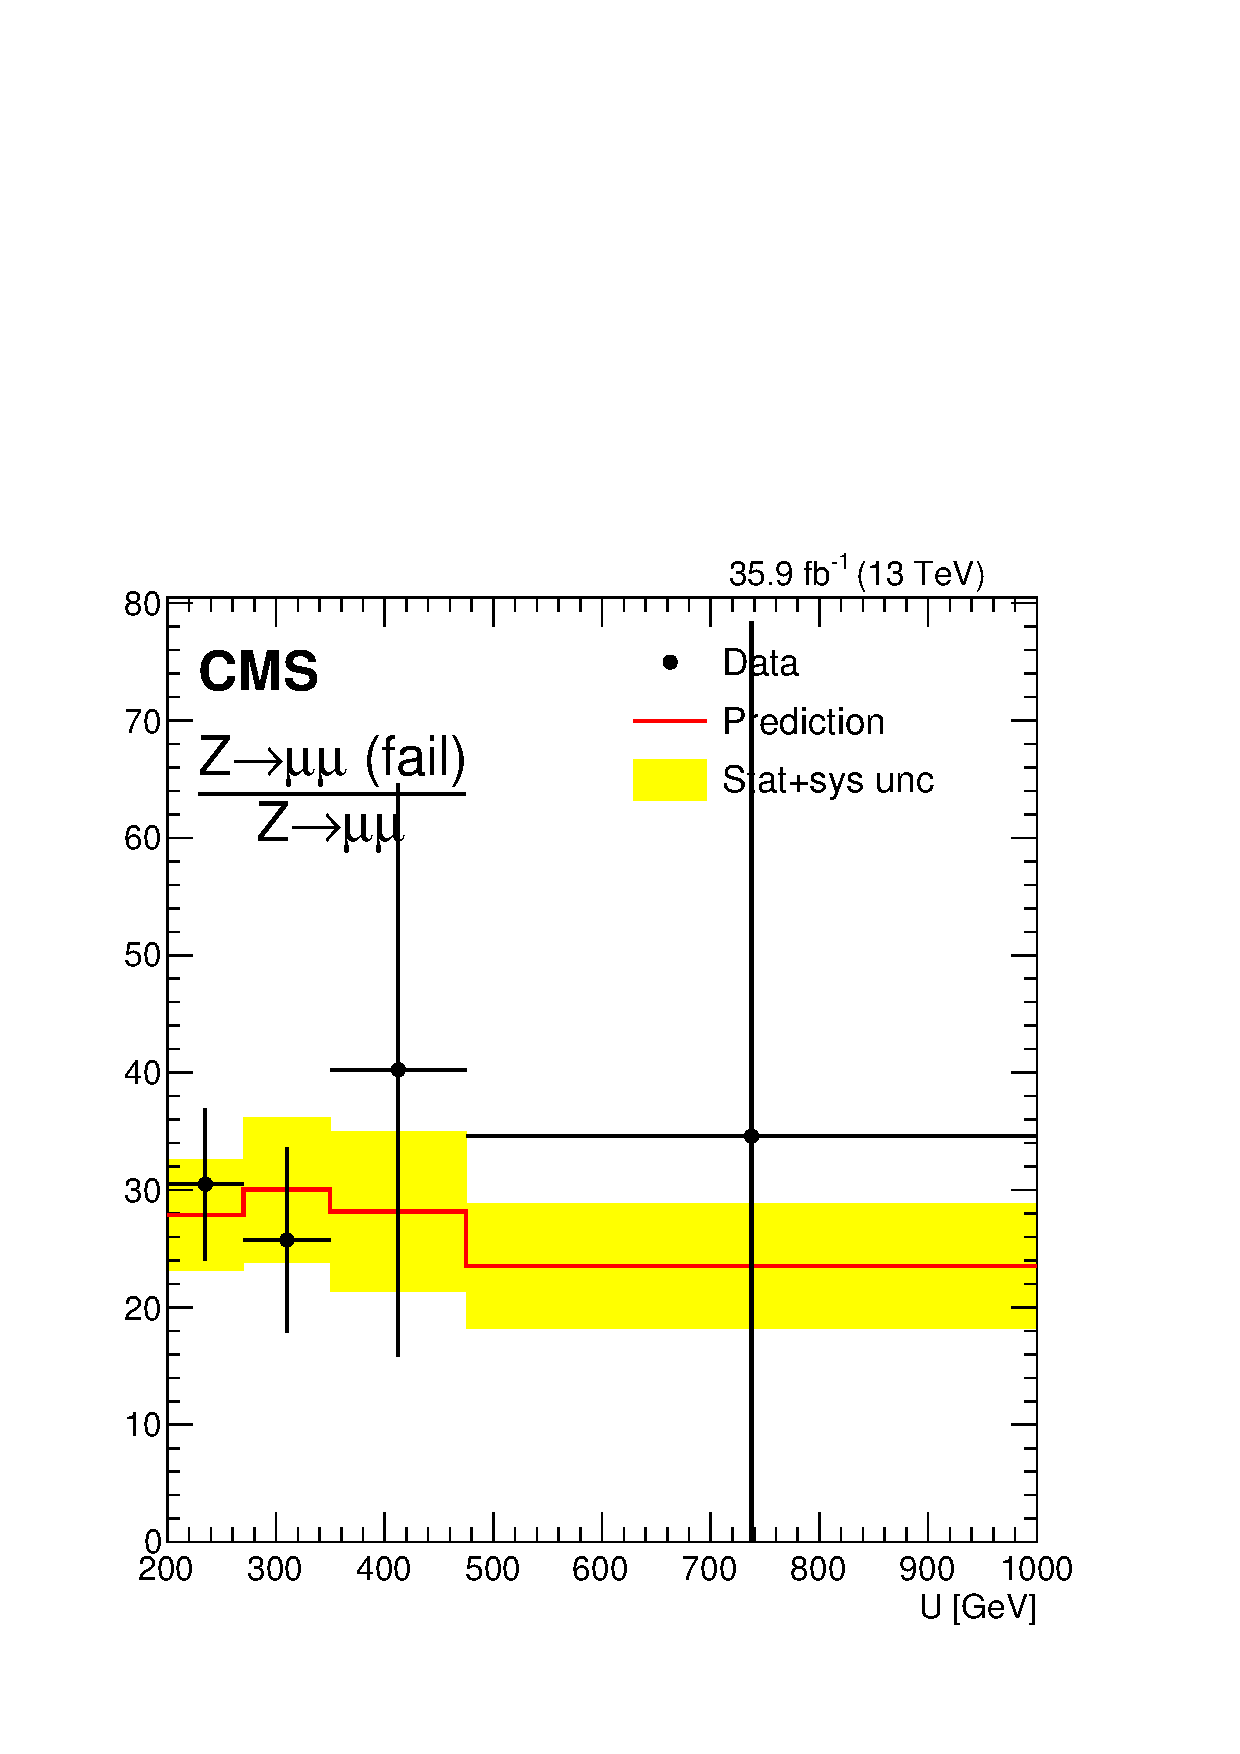
\includegraphics[width=0.45\textwidth]{figures/pullsImpact/ratio_zmm_fail_zmm_shapes_prefit.pdf}
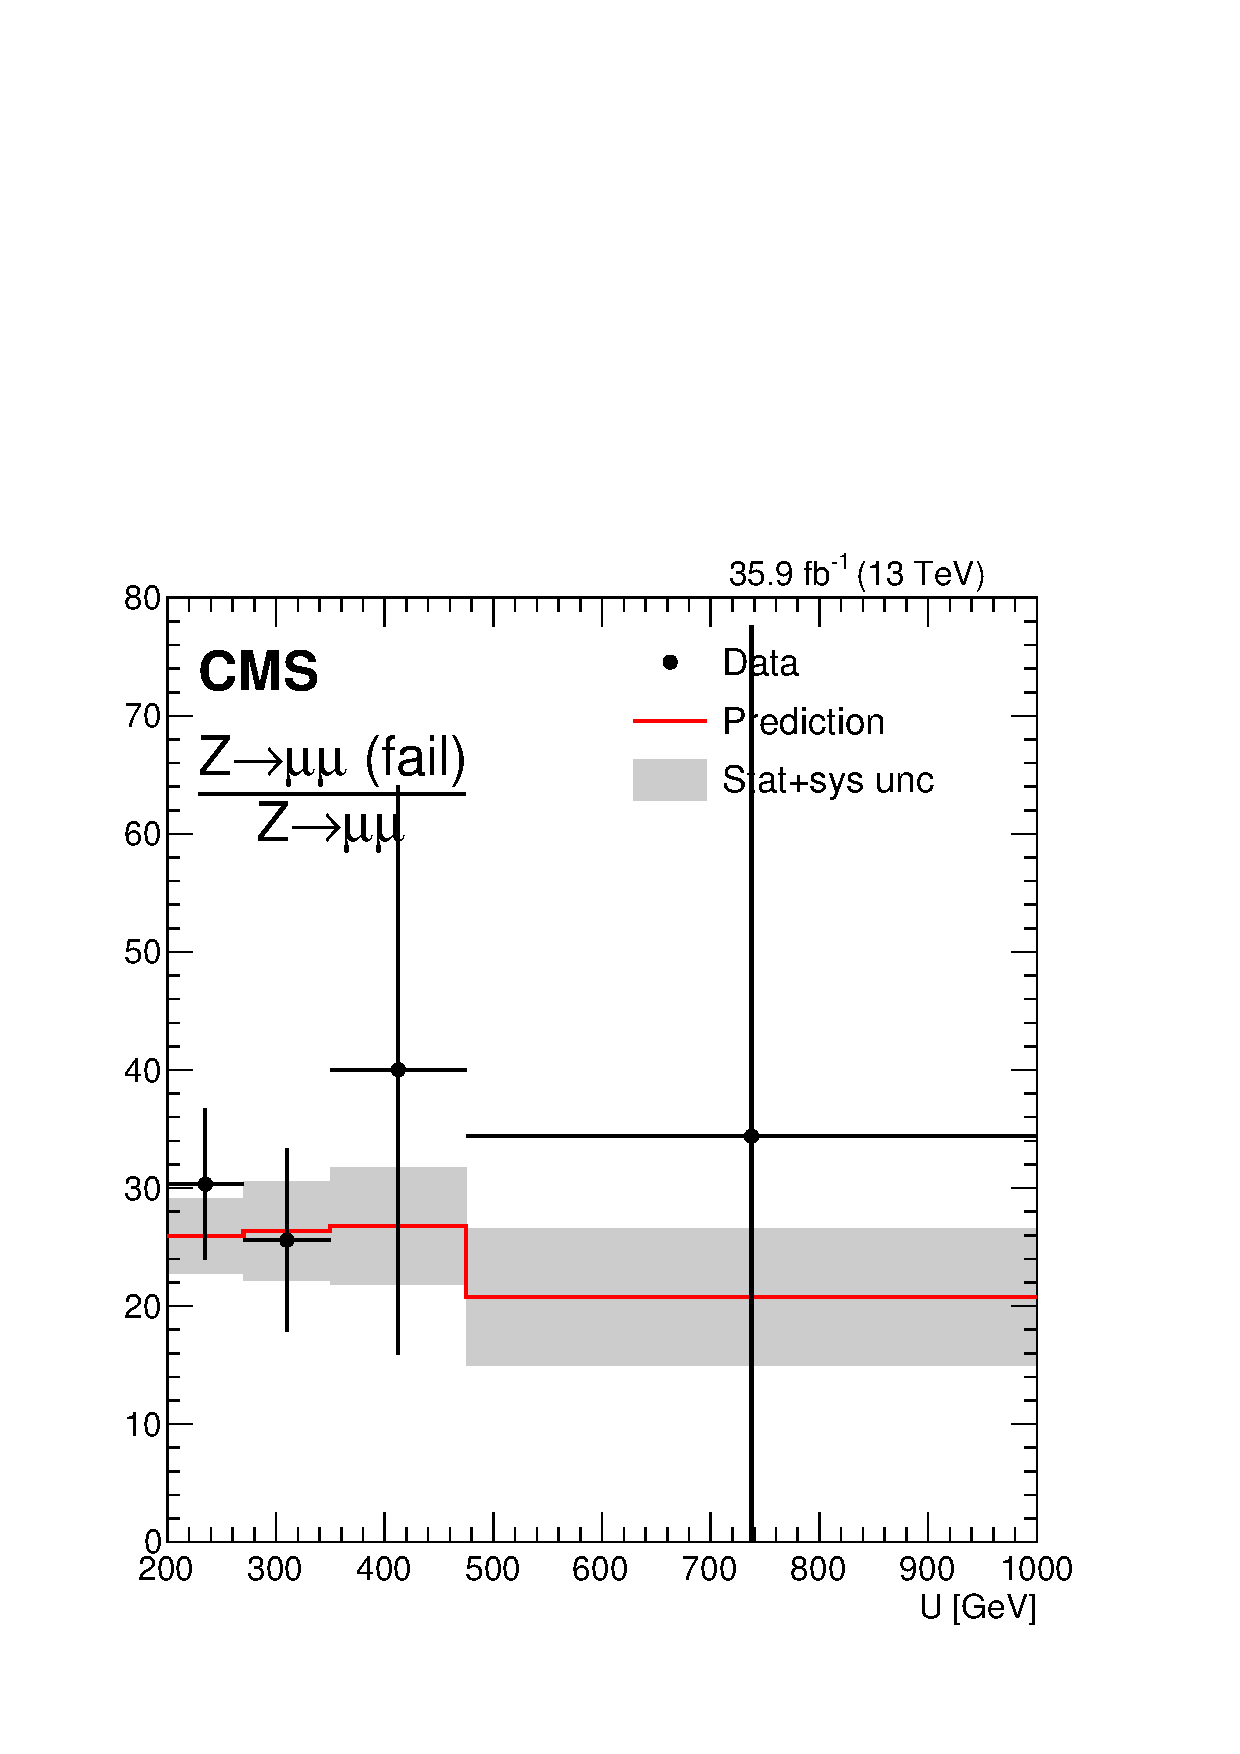
\includegraphics[width=0.45\textwidth]{figures/pullsImpact/ratio_zmm_fail_zmm_shapes_fit_b.pdf}\\
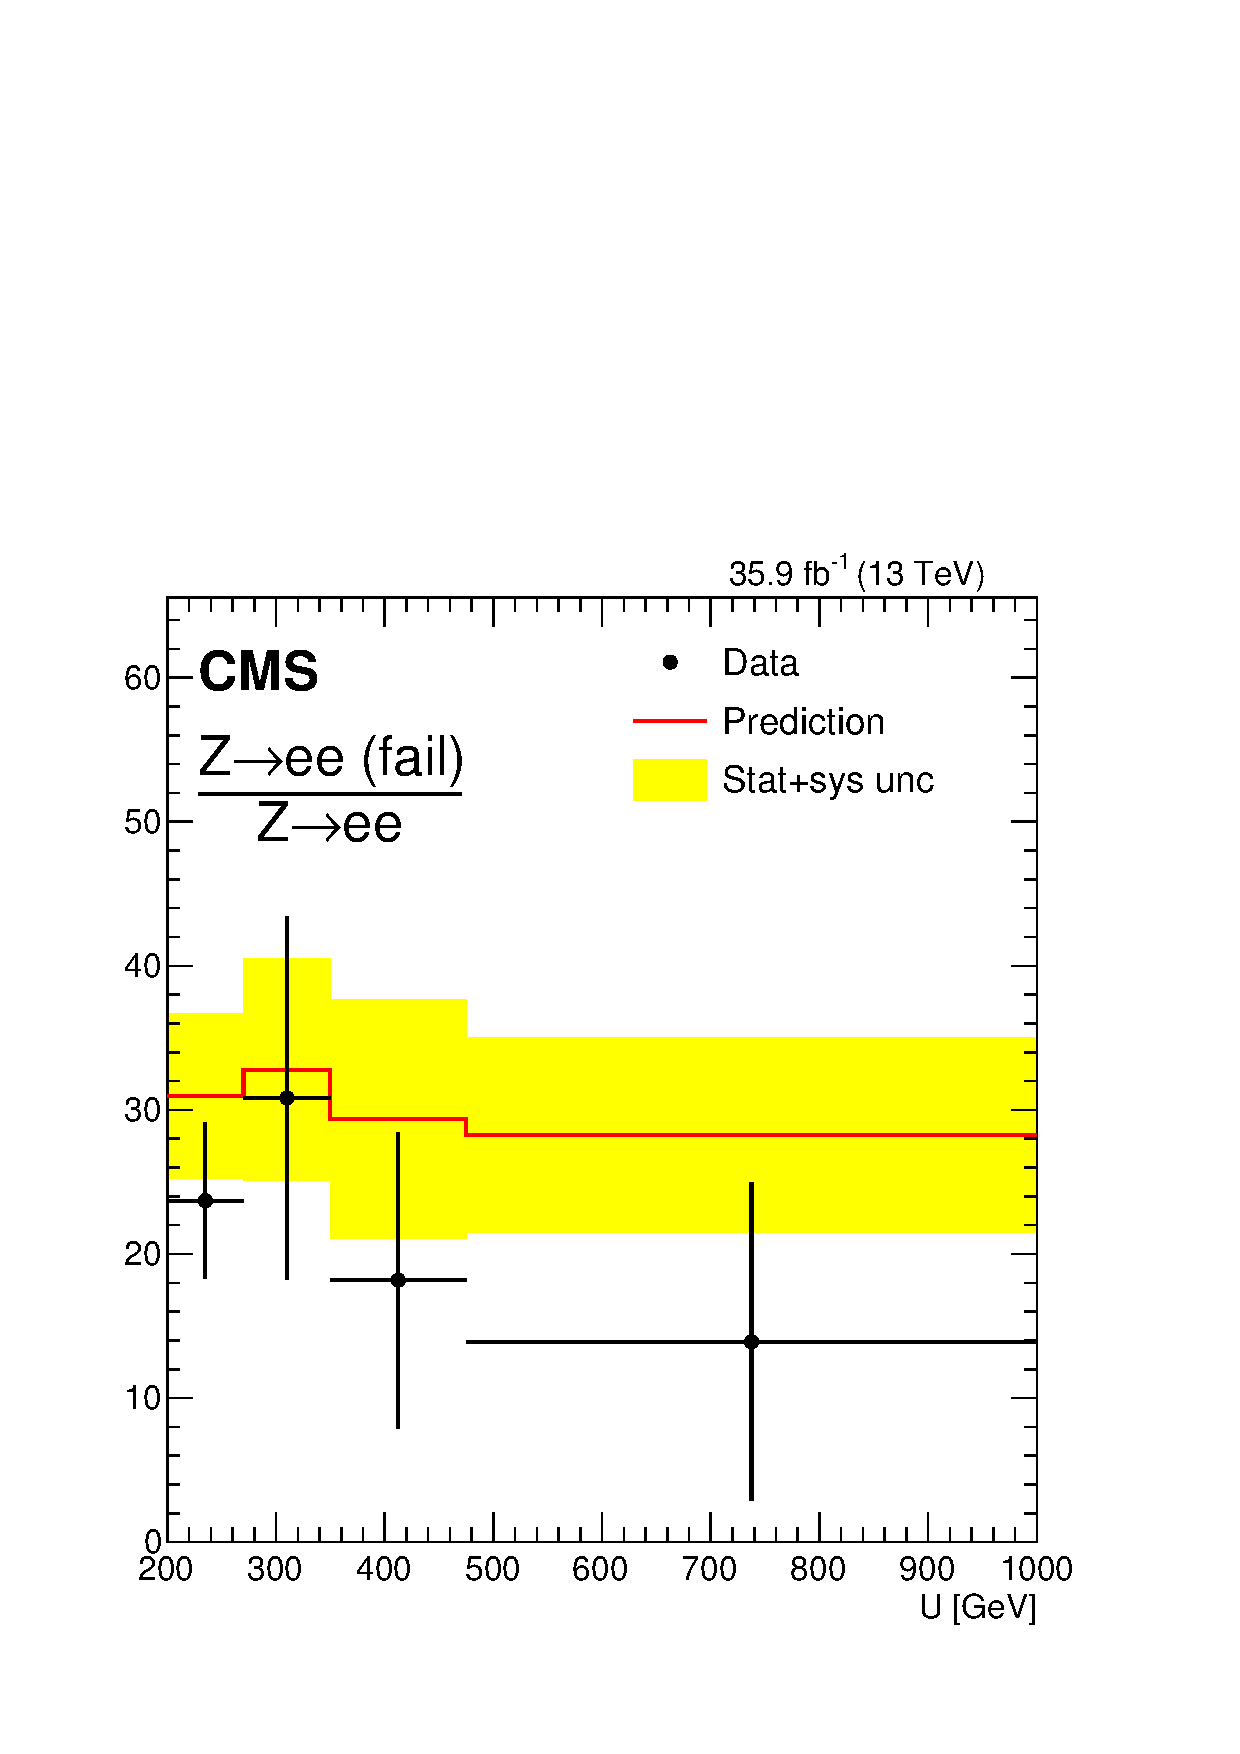
\includegraphics[width=0.45\textwidth]{figures/pullsImpact/ratio_zee_fail_zee_shapes_prefit.pdf}
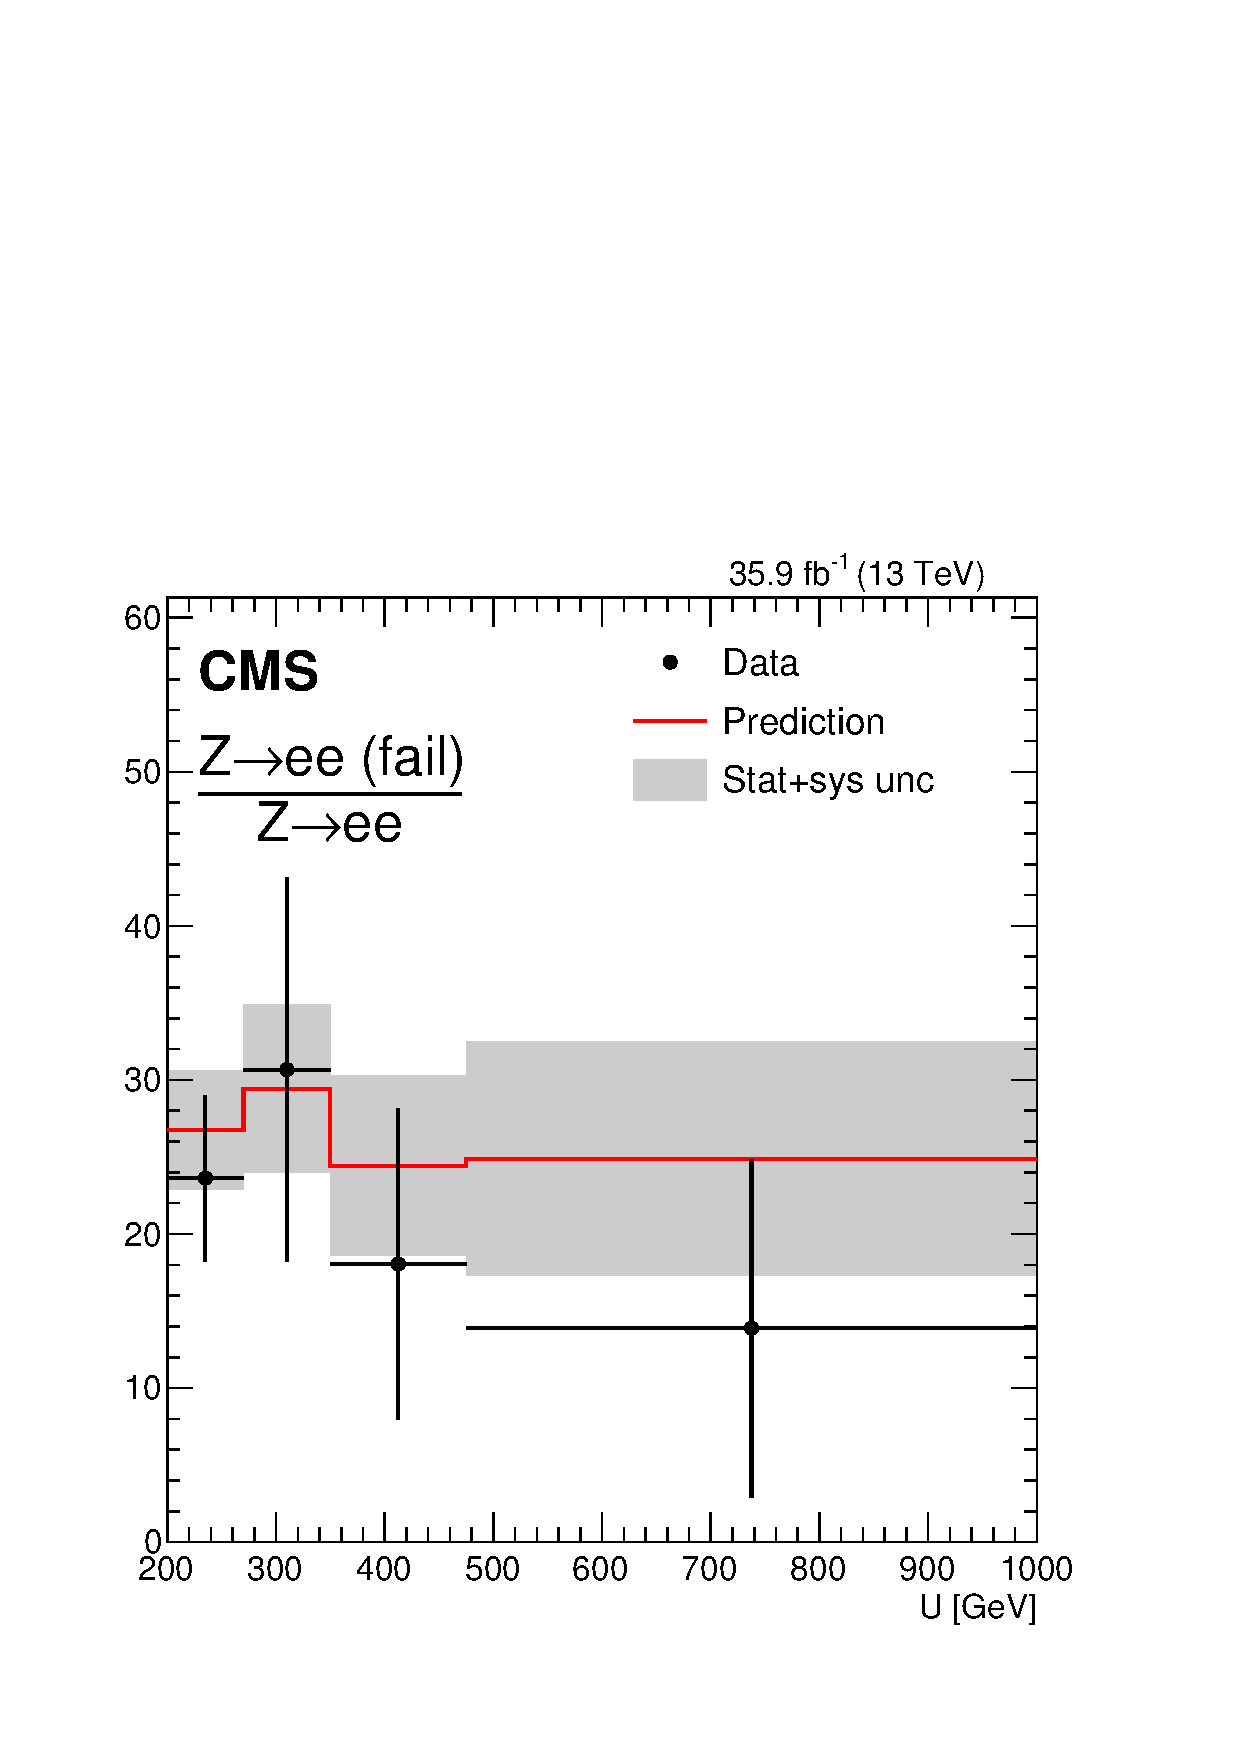
\includegraphics[width=0.45\textwidth]{figures/pullsImpact/ratio_zee_fail_zee_shapes_fit_b.pdf}\\
\caption{Ratios of pre-fit (left column) and post-fit (right column) templates for Z+jets processes in the Z pass/fail regions. Black dots indicate the ratio of data yields (after subtracting trailing backgrounds) and demonstrate good agreement between data and simulation.}
\label{wwratios}
\end{figure}

\clearpage

\begin{figure}
\centering
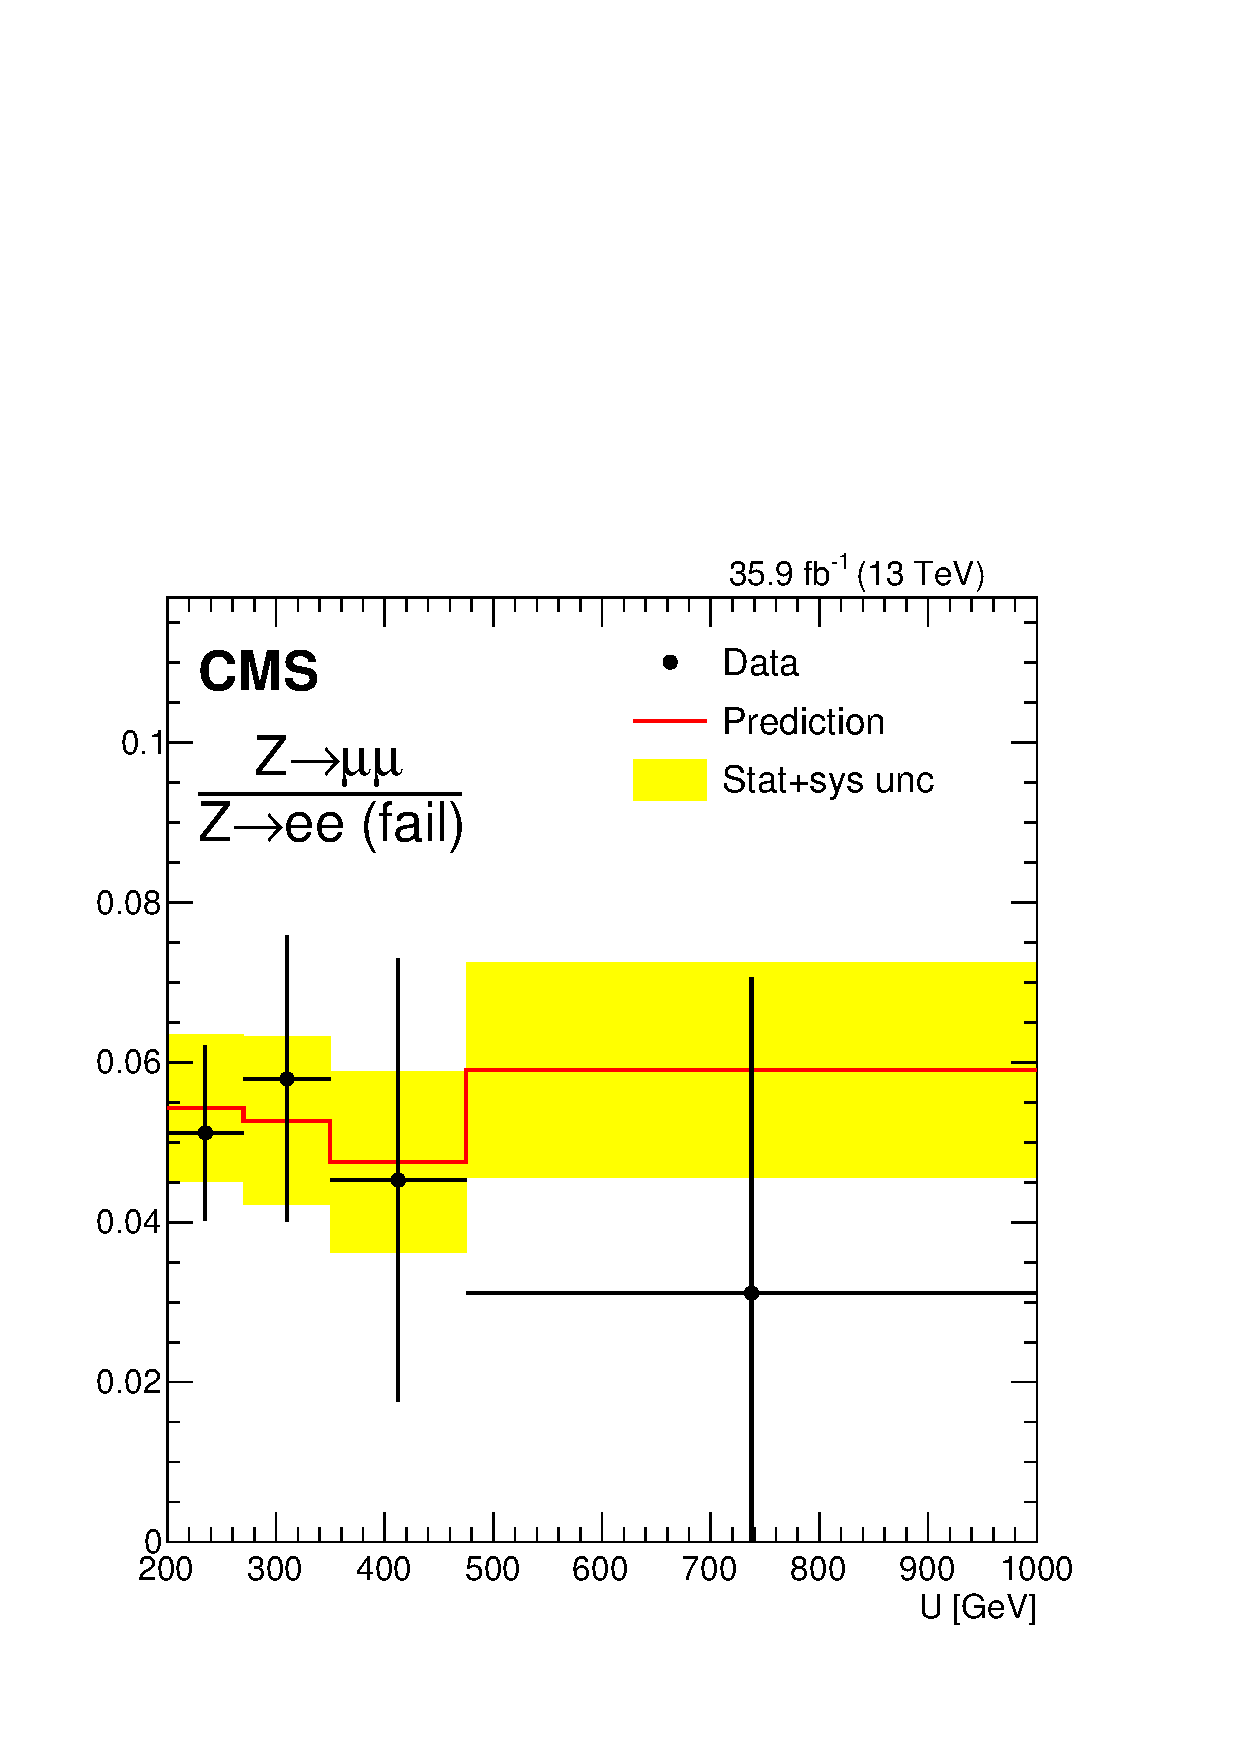
\includegraphics[width=0.45\textwidth]{figures/pullsImpact/ratio_zmm_zee_fail_shapes_prefit.pdf}
\includegraphics[width=0.45\textwidth]{figures/pullsImpact/ratio_zmm_zee_fail_shapes_fit_b.pdf}\\
\includegraphics[width=0.45\textwidth]{figures/pullsImpact/ratio_zmm_fail_zee_shapes_prefit.pdf}
\includegraphics[width=0.45\textwidth]{figures/pullsImpact/ratio_zmm_fail_zee_shapes_fit_b.pdf}\\
\caption{Ratios of pre-fit (left column) and post-fit (right column) templates for Z+jets processes in the Z pass/fail regions. Black dots indicate the ratio of data yields (after subtracting trailing backgrounds) and demonstrate good agreement between data and simulation.}
\label{wwratios}
\end{figure}
